\documentclass[a4paper]{book}
\usepackage{a4wide}
\usepackage{makeidx}
\usepackage{fancyhdr}
\usepackage{graphicx}
\usepackage{multicol}
\usepackage{float}
\usepackage{textcomp}
\usepackage{alltt}
\usepackage[utf8]{inputenc}
\usepackage{doxygen}
\makeindex
\setcounter{tocdepth}{1}
\renewcommand{\footrulewidth}{0.4pt}
\begin{document}
\begin{titlepage}
\vspace*{7cm}
\begin{center}
{\Large ParadisEO-MOMovingObjects Reference Manual\\[1ex]\large 1.0 }\\
\vspace*{1cm}
{\large Generated by Doxygen 1.5.4}\\
\vspace*{0.5cm}
{\small Wed Jan 16 15:50:40 2008}\\
\end{center}
\end{titlepage}
\clearemptydoublepage
\pagenumbering{roman}
\tableofcontents
\clearemptydoublepage
\pagenumbering{arabic}
\chapter{Welcome to PARADISEO-Moving Objects }
\label{index}\section{Introduction}\label{main_Introduction}
The capacitated vehicle routing problem with time windows or CVRP-TW is a combinatorial optimization problem seeking to service a number of customers with a fleet of vehicles where the vehicles have a mimited capacity and the delivery locations have time windows within which the deliveries (or visits) must be made. Often the context is that of delivering goods located at a central depot to customers who have placed orders for such goods. Implicit is the goal of minimizing the cost of distributing the goods. Finding the global minimum for the cost function, except for the smallest instances, is computationally complex.\section{AUTHORS}\label{main_authors}
\begin{TabularC}{3}
\hline
Dolphin project-team INRIA Futurs, 2007. &Antonio La\-Torre atorre[at]fi.upm.es &Thomas Legrand paradiseo-help[at]lists.gforge.inria.fr  \\\hline
\end{TabularC}
\section{LICENSE}\label{main_LICENSE}
This software is governed by the Ce\-CILL license under French law and abiding by the rules of distribution of free software. You can use, modify and/ or redistribute the software under the terms of the Ce\-CILL license as circulated by CEA, CNRS and INRIA at the following URL \char`\"{}http://www.cecill.info\char`\"{}.

As a counterpart to the access to the source code and rights to copy, modify and redistribute granted by the license, users are provided only with a limited warranty and the software's author, the holder of the economic rights, and the successive licensors have only limited liability.

In this respect, the user's attention is drawn to the risks associated with loading, using, modifying and/or developing or reproducing the software by the user in light of its specific status of free software, that may mean that it is complicated to manipulate, and that also therefore means that it is reserved for developers and experienced professionals having in-depth computer knowledge. Users are therefore encouraged to load and test the software's suitability as regards their requirements in conditions enabling the security of their systems and/or data to be ensured and, more generally, to use and operate it in the same conditions as regards security. The fact that you are presently reading this means that you have had knowledge of the Ce\-CILL license and that you accept its terms.

Paradis\-EO Web\-Site : \tt{http://paradiseo.gforge.inria.fr} Contact: \tt{paradiseo-help@lists.gforge.inria.fr}\section{Home Page}\label{main_Paradiseo}
{\tt http://paradiseo.gforge.inria.fr} 
\chapter{ParadisEO-MOMovingObjects Hierarchical Index}
\section{Paradis\-EO-MO-Moving\-Objects Class Hierarchy}
This inheritance list is sorted roughly, but not completely, alphabetically:\begin{CompactList}
\item \contentsline{section}{mo\-Algo$<$ EOT $>$}{\pageref{classmo_algo}}{}
\item \contentsline{section}{mo\-Aspir\-Crit$<$ M $>$}{\pageref{classmo_aspir_crit}}{}
\begin{CompactList}
\item \contentsline{section}{mo\-Impr\-Best\-Fit\-Aspir\-Crit$<$ M $>$}{\pageref{classmo_impr_best_fit_aspir_crit}}{}
\item \contentsline{section}{mo\-No\-Aspir\-Crit$<$ M $>$}{\pageref{classmo_no_aspir_crit}}{}
\end{CompactList}
\item \contentsline{section}{mo\-Comparator$<$ EOT $>$}{\pageref{classmo_comparator}}{}
\begin{CompactList}
\item \contentsline{section}{mo\-Fit\-Comparator$<$ EOT $>$}{\pageref{classmo_fit_comparator}}{}
\end{CompactList}
\item \contentsline{section}{mo\-Cooling\-Schedule}{\pageref{classmo_cooling_schedule}}{}
\begin{CompactList}
\item \contentsline{section}{mo\-Exponential\-Cooling\-Schedule}{\pageref{classmo_exponential_cooling_schedule}}{}
\item \contentsline{section}{mo\-Linear\-Cooling\-Schedule}{\pageref{classmo_linear_cooling_schedule}}{}
\end{CompactList}
\item \contentsline{section}{mo\-HC$<$ M $>$}{\pageref{classmo_h_c}}{}
\item \contentsline{section}{mo\-ILS$<$ M $>$}{\pageref{classmo_i_l_s}}{}
\item \contentsline{section}{mo\-LSCheck\-Point$<$ M $>$}{\pageref{classmo_l_s_check_point}}{}
\item \contentsline{section}{mo\-Move$<$ EOT $>$}{\pageref{classmo_move}}{}
\item \contentsline{section}{mo\-Move\-Expl$<$ M $>$}{\pageref{classmo_move_expl}}{}
\begin{CompactList}
\item \contentsline{section}{mo\-Move\-Loop\-Expl$<$ M $>$}{\pageref{classmo_move_loop_expl}}{}
\begin{CompactList}
\item \contentsline{section}{mo\-HCMove\-Loop\-Expl$<$ M $>$}{\pageref{classmo_h_c_move_loop_expl}}{}
\item \contentsline{section}{mo\-TSMove\-Loop\-Expl$<$ M $>$}{\pageref{classmo_t_s_move_loop_expl}}{}
\end{CompactList}
\end{CompactList}
\item \contentsline{section}{mo\-Move\-Incr\-Eval$<$ M $>$}{\pageref{classmo_move_incr_eval}}{}
\item \contentsline{section}{mo\-Move\-Init$<$ M $>$}{\pageref{classmo_move_init}}{}
\item \contentsline{section}{mo\-Move\-Select$<$ M $>$}{\pageref{classmo_move_select}}{}
\begin{CompactList}
\item \contentsline{section}{mo\-Best\-Impr\-Select$<$ M $>$}{\pageref{classmo_best_impr_select}}{}
\item \contentsline{section}{mo\-First\-Impr\-Select$<$ M $>$}{\pageref{classmo_first_impr_select}}{}
\item \contentsline{section}{mo\-Rand\-Impr\-Select$<$ M $>$}{\pageref{classmo_rand_impr_select}}{}
\end{CompactList}
\item \contentsline{section}{mo\-Next\-Move$<$ M $>$}{\pageref{classmo_next_move}}{}
\begin{CompactList}
\item \contentsline{section}{mo\-It\-Rand\-Next\-Move$<$ M $>$}{\pageref{classmo_it_rand_next_move}}{}
\end{CompactList}
\item \contentsline{section}{mo\-Rand\-Move$<$ M $>$}{\pageref{classmo_rand_move}}{}
\item \contentsline{section}{mo\-SA$<$ M $>$}{\pageref{classmo_s_a}}{}
\item \contentsline{section}{mo\-Sol\-Continue$<$ EOT $>$}{\pageref{classmo_sol_continue}}{}
\begin{CompactList}
\item \contentsline{section}{mo\-Fit\-Sol\-Continue$<$ EOT $>$}{\pageref{classmo_fit_sol_continue}}{}
\item \contentsline{section}{mo\-Gen\-Sol\-Continue$<$ EOT $>$}{\pageref{classmo_gen_sol_continue}}{}
\item \contentsline{section}{mo\-No\-Fit\-Impr\-Sol\-Continue$<$ EOT $>$}{\pageref{classmo_no_fit_impr_sol_continue}}{}
\item \contentsline{section}{mo\-Steady\-Fit\-Sol\-Continue$<$ EOT $>$}{\pageref{classmo_steady_fit_sol_continue}}{}
\end{CompactList}
\item \contentsline{section}{mo\-Tabu\-List$<$ M $>$}{\pageref{classmo_tabu_list}}{}
\begin{CompactList}
\item \contentsline{section}{mo\-Simple\-Move\-Tabu\-List$<$ M $>$}{\pageref{classmo_simple_move_tabu_list}}{}
\item \contentsline{section}{mo\-Simple\-Solution\-Tabu\-List$<$ M $>$}{\pageref{classmo_simple_solution_tabu_list}}{}
\end{CompactList}
\item \contentsline{section}{mo\-TS$<$ M $>$}{\pageref{classmo_t_s}}{}
\end{CompactList}

\chapter{ParadisEO-MOMovingObjects Class Index}
\section{Paradis\-EO-PEO-Parallelanddistributed\-Evolving\-Objects Class List}
Here are the classes, structs, unions and interfaces with brief descriptions:\begin{CompactList}
\item\contentsline{section}{\hyperlink{structAlgorithm}{Algorithm} }{\pageref{structAlgorithm}}{}
\item\contentsline{section}{\hyperlink{classCitySwap}{City\-Swap} (Its swaps two vertices randomly choosen )}{\pageref{classCitySwap}}{}
\item\contentsline{section}{\hyperlink{classCommunicable}{Communicable} }{\pageref{classCommunicable}}{}
\item\contentsline{section}{\hyperlink{classCommunicator}{Communicator} }{\pageref{classCommunicator}}{}
\item\contentsline{section}{\hyperlink{classCompleteTopology}{Complete\-Topology} }{\pageref{classCompleteTopology}}{}
\item\contentsline{section}{\hyperlink{classcontinuator}{continuator} (Abstract class for a continuator within the exchange of data by migration )}{\pageref{classcontinuator}}{}
\item\contentsline{section}{\hyperlink{classCooperative}{Cooperative} }{\pageref{classCooperative}}{}
\item\contentsline{section}{\hyperlink{classDisplayBestRoute}{Display\-Best\-Route} }{\pageref{classDisplayBestRoute}}{}
\item\contentsline{section}{\hyperlink{classEdgeXover}{Edge\-Xover} (Edge Crossover )}{\pageref{classEdgeXover}}{}
\item\contentsline{section}{\hyperlink{classeoContinuator}{eo\-Continuator$<$ EOT $>$} (Specific class for a continuator within the exchange of migration of a population )}{\pageref{classeoContinuator}}{}
\item\contentsline{section}{\hyperlink{classeoReplace}{eo\-Replace$<$ EOT, TYPE $>$} (Specific class for a replacement within the exchange of migration of a population )}{\pageref{classeoReplace}}{}
\item\contentsline{section}{\hyperlink{classeoSelector}{eo\-Selector$<$ EOT, TYPE $>$} (Specific class for a selector within the exchange of migration of a population )}{\pageref{classeoSelector}}{}
\item\contentsline{section}{\hyperlink{classeoSyncContinue}{eo\-Sync\-Continue} (Class for a continuator within the exchange of data by synchrone migration )}{\pageref{classeoSyncContinue}}{}
\item\contentsline{section}{\hyperlink{classMergeRouteEval}{Merge\-Route\-Eval} }{\pageref{classMergeRouteEval}}{}
\item\contentsline{section}{\hyperlink{classMPIThreadedEnv}{MPIThreaded\-Env} }{\pageref{classMPIThreadedEnv}}{}
\item\contentsline{section}{\hyperlink{classOrderXover}{Order\-Xover} (Order Crossover )}{\pageref{classOrderXover}}{}
\item\contentsline{section}{\hyperlink{classPartialMappedXover}{Partial\-Mapped\-Xover} (Partial Mapped Crossover )}{\pageref{classPartialMappedXover}}{}
\item\contentsline{section}{\hyperlink{classPartRouteEval}{Part\-Route\-Eval} (Route Evaluator )}{\pageref{classPartRouteEval}}{}
\item\contentsline{section}{\hyperlink{classpeoAggEvalFunc}{peo\-Agg\-Eval\-Func$<$ EOT $>$} (The \hyperlink{classpeoAggEvalFunc}{peo\-Agg\-Eval\-Func} class offers only the interface for creating aggregate evaluation functions - there are no direct internal functions provided )}{\pageref{classpeoAggEvalFunc}}{}
\item\contentsline{section}{\hyperlink{classpeoAsyncIslandMig}{peo\-Async\-Island\-Mig$<$ TYPESELECT, TYPEREPLACE $>$} (Specific class for a asynchronous migration )}{\pageref{classpeoAsyncIslandMig}}{}
\item\contentsline{section}{\hyperlink{structpeoEvalFunc}{peo\-Eval\-Func$<$ EOT, Fit\-T, Function\-Arg $>$} (Specific class for evaluation )}{\pageref{structpeoEvalFunc}}{}
\item\contentsline{section}{\hyperlink{classpeoGlobalBestVelocity}{peo\-Global\-Best\-Velocity$<$ POT $>$} (Specific class for a replacement thanks to the velocity migration of a population of a PSO )}{\pageref{classpeoGlobalBestVelocity}}{}
\item\contentsline{section}{\hyperlink{classpeoMultiStart}{peo\-Multi\-Start$<$ Entity\-Type $>$} (Class allowing the launch of several algorithms )}{\pageref{classpeoMultiStart}}{}
\item\contentsline{section}{\hyperlink{structpeoMultiStart_1_1AbstractAggregationAlgorithm}{peo\-Multi\-Start$<$ Entity\-Type $>$::Abstract\-Aggregation\-Algorithm} }{\pageref{structpeoMultiStart_1_1AbstractAggregationAlgorithm}}{}
\item\contentsline{section}{\hyperlink{structpeoMultiStart_1_1AbstractAlgorithm}{peo\-Multi\-Start$<$ Entity\-Type $>$::Abstract\-Algorithm} }{\pageref{structpeoMultiStart_1_1AbstractAlgorithm}}{}
\item\contentsline{section}{\hyperlink{structpeoMultiStart_1_1AbstractDataType}{peo\-Multi\-Start$<$ Entity\-Type $>$::Abstract\-Data\-Type} }{\pageref{structpeoMultiStart_1_1AbstractDataType}}{}
\item\contentsline{section}{\hyperlink{structpeoMultiStart_1_1AggregationAlgorithm}{peo\-Multi\-Start$<$ Entity\-Type $>$::Aggregation\-Algorithm$<$ Aggregation\-Algorithm\-Type $>$} }{\pageref{structpeoMultiStart_1_1AggregationAlgorithm}}{}
\item\contentsline{section}{\hyperlink{structpeoMultiStart_1_1Algorithm}{peo\-Multi\-Start$<$ Entity\-Type $>$::Algorithm$<$ Algorithm\-Type $>$} }{\pageref{structpeoMultiStart_1_1Algorithm}}{}
\item\contentsline{section}{\hyperlink{structpeoMultiStart_1_1DataType}{peo\-Multi\-Start$<$ Entity\-Type $>$::Data\-Type$<$ Type $>$} }{\pageref{structpeoMultiStart_1_1DataType}}{}
\item\contentsline{section}{\hyperlink{structpeoMultiStart_1_1FunctionAlgorithm}{peo\-Multi\-Start$<$ Entity\-Type $>$::Function\-Algorithm$<$ Algorithm\-Return\-Type, Algorithm\-Data\-Type $>$} }{\pageref{structpeoMultiStart_1_1FunctionAlgorithm}}{}
\item\contentsline{section}{\hyperlink{structpeoMultiStart_1_1NoAggregationFunction}{peo\-Multi\-Start$<$ Entity\-Type $>$::No\-Aggregation\-Function} }{\pageref{structpeoMultiStart_1_1NoAggregationFunction}}{}
\item\contentsline{section}{\hyperlink{classpeoNoAggEvalFunc}{peo\-No\-Agg\-Eval\-Func$<$ EOT $>$} (The \hyperlink{classpeoNoAggEvalFunc}{peo\-No\-Agg\-Eval\-Func} class does nothing more than an association between a fitness value and a specified individual )}{\pageref{classpeoNoAggEvalFunc}}{}
\item\contentsline{section}{\hyperlink{classpeoPopEval}{peo\-Pop\-Eval$<$ EOT $>$} (Parallel evaluation functor wrapper )}{\pageref{classpeoPopEval}}{}
\item\contentsline{section}{\hyperlink{classpeoPSOSelect}{peo\-PSOSelect$<$ POT $>$} (Specific class for a selection of a population of a PSO )}{\pageref{classpeoPSOSelect}}{}
\item\contentsline{section}{\hyperlink{classpeoSyncIslandMig}{peo\-Sync\-Island\-Mig$<$ TYPESELECT, TYPEREPLACE $>$} (Specific class for a synchronous migration )}{\pageref{classpeoSyncIslandMig}}{}
\item\contentsline{section}{\hyperlink{classpeoTransform}{peo\-Transform$<$ EOT $>$} (Class for a parallel transform )}{\pageref{classpeoTransform}}{}
\item\contentsline{section}{\hyperlink{classpeoWorstPositionReplacement}{peo\-Worst\-Position\-Replacement$<$ POT $>$} (Specific class for a replacement of a population of a PSO )}{\pageref{classpeoWorstPositionReplacement}}{}
\item\contentsline{section}{\hyperlink{classpeoWrapper}{peo\-Wrapper} (Specific class for wrapping )}{\pageref{classpeoWrapper}}{}
\item\contentsline{section}{\hyperlink{structpeoWrapper_1_1AbstractAlgorithm}{peo\-Wrapper::Abstract\-Algorithm} }{\pageref{structpeoWrapper_1_1AbstractAlgorithm}}{}
\item\contentsline{section}{\hyperlink{structpeoWrapper_1_1Algorithm}{peo\-Wrapper::Algorithm$<$ Algorithm\-Type, Algorithm\-Data\-Type $>$} }{\pageref{structpeoWrapper_1_1Algorithm}}{}
\item\contentsline{section}{\hyperlink{structpeoWrapper_1_1Algorithm_3_01AlgorithmType_00_01void_01_4}{peo\-Wrapper::Algorithm$<$ Algorithm\-Type, void $>$} }{\pageref{structpeoWrapper_1_1Algorithm_3_01AlgorithmType_00_01void_01_4}}{}
\item\contentsline{section}{\hyperlink{structpeoWrapper_1_1FunctionAlgorithm}{peo\-Wrapper::Function\-Algorithm$<$ Algorithm\-Return\-Type, Algorithm\-Data\-Type $>$} }{\pageref{structpeoWrapper_1_1FunctionAlgorithm}}{}
\item\contentsline{section}{\hyperlink{structpeoWrapper_1_1FunctionAlgorithm_3_01AlgorithmReturnType_00_01void_01_4}{peo\-Wrapper::Function\-Algorithm$<$ Algorithm\-Return\-Type, void $>$} }{\pageref{structpeoWrapper_1_1FunctionAlgorithm_3_01AlgorithmReturnType_00_01void_01_4}}{}
\item\contentsline{section}{\hyperlink{classRandomTopology}{Random\-Topology} }{\pageref{classRandomTopology}}{}
\item\contentsline{section}{\hyperlink{classReactiveThread}{Reactive\-Thread} }{\pageref{classReactiveThread}}{}
\item\contentsline{section}{\hyperlink{classreplacement}{replacement$<$ TYPE $>$} (Abstract class for a replacement within the exchange of data by migration )}{\pageref{classreplacement}}{}
\item\contentsline{section}{\hyperlink{classRingTopology}{Ring\-Topology} }{\pageref{classRingTopology}}{}
\item\contentsline{section}{\hyperlink{classRouteEval}{Route\-Eval} }{\pageref{classRouteEval}}{}
\item\contentsline{section}{\hyperlink{classRouteInit}{Route\-Init} }{\pageref{classRouteInit}}{}
\item\contentsline{section}{\hyperlink{classRunner}{Runner} }{\pageref{classRunner}}{}
\item\contentsline{section}{\hyperlink{classselector}{selector$<$ TYPE $>$} (Abstract class for a selector within the exchange of data by migration )}{\pageref{classselector}}{}
\item\contentsline{section}{\hyperlink{structSEND__REQUEST}{SEND\_\-REQUEST} }{\pageref{structSEND__REQUEST}}{}
\item\contentsline{section}{\hyperlink{classService}{Service} }{\pageref{classService}}{}
\item\contentsline{section}{\hyperlink{classStarTopology}{Star\-Topology} }{\pageref{classStarTopology}}{}
\item\contentsline{section}{\hyperlink{structSyncCompare}{Sync\-Compare} }{\pageref{structSyncCompare}}{}
\item\contentsline{section}{\hyperlink{structSyncEntry}{Sync\-Entry} }{\pageref{structSyncEntry}}{}
\item\contentsline{section}{\hyperlink{classThread}{Thread} }{\pageref{classThread}}{}
\item\contentsline{section}{\hyperlink{classTopology}{Topology} }{\pageref{classTopology}}{}
\item\contentsline{section}{\hyperlink{classTwoOpt}{Two\-Opt} }{\pageref{classTwoOpt}}{}
\item\contentsline{section}{\hyperlink{classTwoOptIncrEval}{Two\-Opt\-Incr\-Eval} }{\pageref{classTwoOptIncrEval}}{}
\item\contentsline{section}{\hyperlink{classTwoOptInit}{Two\-Opt\-Init} }{\pageref{classTwoOptInit}}{}
\item\contentsline{section}{\hyperlink{classTwoOptNext}{Two\-Opt\-Next} }{\pageref{classTwoOptNext}}{}
\item\contentsline{section}{\hyperlink{classTwoOptRand}{Two\-Opt\-Rand} }{\pageref{classTwoOptRand}}{}
\item\contentsline{section}{\hyperlink{classWorker}{Worker} }{\pageref{classWorker}}{}
\end{CompactList}

\chapter{ParadisEO-MOMovingObjects Class Documentation}
\section{mo\-Algo$<$ EOT $>$ Class Template Reference}
\label{classmo_algo}\index{moAlgo@{moAlgo}}
Description of an algorithm of the paradiseo-mo library.  


{\tt \#include $<$mo\-Algo.h$>$}

Inheritance diagram for mo\-Algo$<$ EOT $>$::\begin{figure}[H]
\begin{center}
\leavevmode
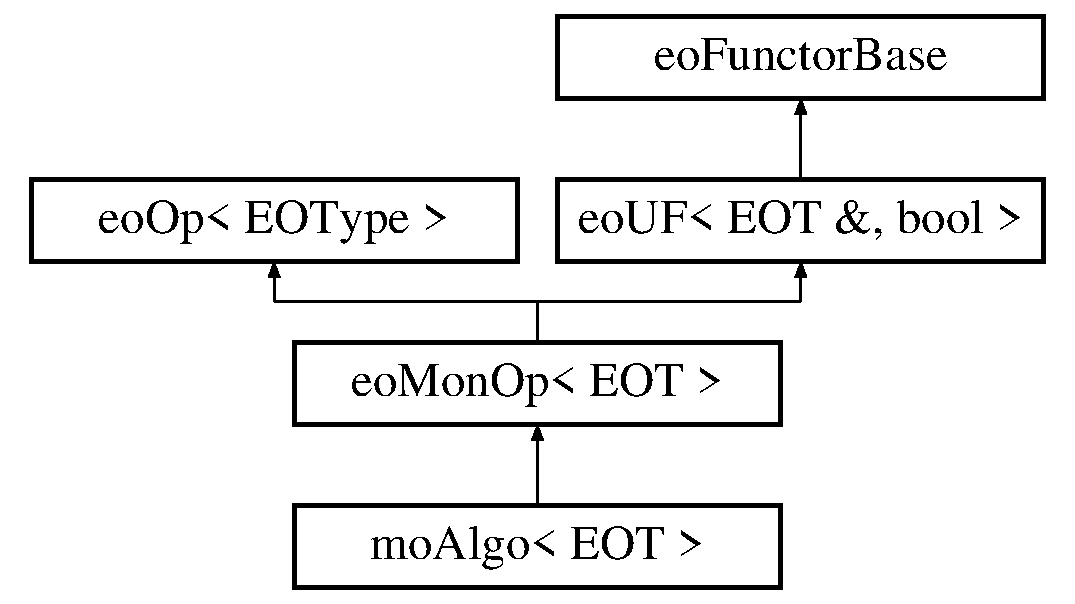
\includegraphics[height=4cm]{classmo_algo}
\end{center}
\end{figure}


\subsection{Detailed Description}
\subsubsection*{template$<$class EOT$>$ class mo\-Algo$<$ EOT $>$}

Description of an algorithm of the paradiseo-mo library. 

{\bf mo\-HC}{\rm (p.\,\pageref{classmo_h_c})}, {\bf mo\-TS}{\rm (p.\,\pageref{classmo_t_s})} and {\bf mo\-SA}{\rm (p.\,\pageref{classmo_s_a})} are 3 examples of algorithm of the paradiseo-mo library. 



Definition at line 46 of file mo\-Algo.h.

The documentation for this class was generated from the following file:\begin{CompactItemize}
\item 
mo\-Algo.h\end{CompactItemize}

\section{mo\-Aspir\-Crit$<$ M $>$ Class Template Reference}
\label{classmo_aspir_crit}\index{moAspirCrit@{moAspirCrit}}
Description of the conditions in which a tabu move could be accepted.  


{\tt \#include $<$mo\-Aspir\-Crit.h$>$}

Inheritance diagram for mo\-Aspir\-Crit$<$ M $>$::\begin{figure}[H]
\begin{center}
\leavevmode
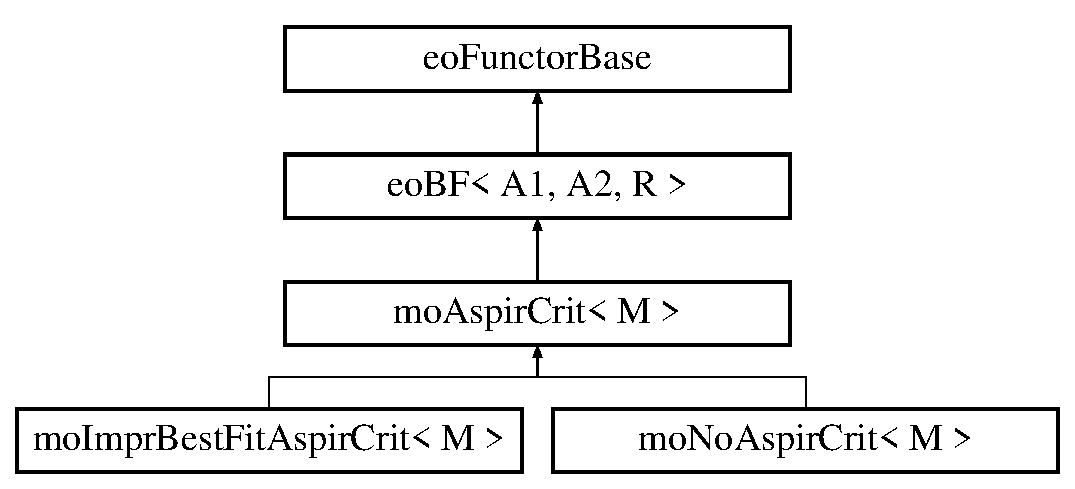
\includegraphics[height=2cm]{classmo_aspir_crit}
\end{center}
\end{figure}
\subsection*{Public Member Functions}
\begin{CompactItemize}
\item 
virtual void \bf{init} ()=0
\begin{CompactList}\small\item\em Procedure which initialises all that needs an aspiration criterion. \item\end{CompactList}\end{CompactItemize}


\subsection{Detailed Description}
\subsubsection*{template$<$class M$>$ class mo\-Aspir\-Crit$<$ M $>$}

Description of the conditions in which a tabu move could be accepted. 

It is only a description... An object that herits from this class is needed to be used in a \doxyref{mo\-TS}{p.}{classmo_t_s}. See mo\-No\-Aspri\-Crit for example. 



Definition at line 47 of file mo\-Aspir\-Crit.h.

\subsection{Member Function Documentation}
\index{moAspirCrit@{mo\-Aspir\-Crit}!init@{init}}
\index{init@{init}!moAspirCrit@{mo\-Aspir\-Crit}}
\subsubsection{\setlength{\rightskip}{0pt plus 5cm}template$<$class M$>$ virtual void \bf{mo\-Aspir\-Crit}$<$ M $>$::init ()\hspace{0.3cm}{\tt  [pure virtual]}}\label{classmo_aspir_crit_a8ce84510a5ec7c9078381e542c6d140}


Procedure which initialises all that needs an aspiration criterion. 

It can be possible that this procedure does nothing... 

Implemented in \bf{mo\-Impr\-Best\-Fit\-Aspir\-Crit$<$ M $>$} \doxyref{p.}{classmo_impr_best_fit_aspir_crit_ffa451a14ff4ea86fb8bd9fdbc348630}, and \bf{mo\-No\-Aspir\-Crit$<$ M $>$} \doxyref{p.}{classmo_no_aspir_crit_f3a286fc4c2d36bd390ba9a3074f3037}.

The documentation for this class was generated from the following file:\begin{CompactItemize}
\item 
mo\-Aspir\-Crit.h\end{CompactItemize}

\section{moBestImprSelect$<$ M $>$ Class Template Reference}
\label{classmo_best_impr_select}\index{moBestImprSelect@{moBestImprSelect}}
One of the possible \doxyref{moMoveSelect}{p.}{classmo_move_select}.  


{\tt \#include $<$moBestImprSelect.h$>$}

Inheritance diagram for moBestImprSelect$<$ M $>$::\begin{figure}[H]
\begin{center}
\leavevmode
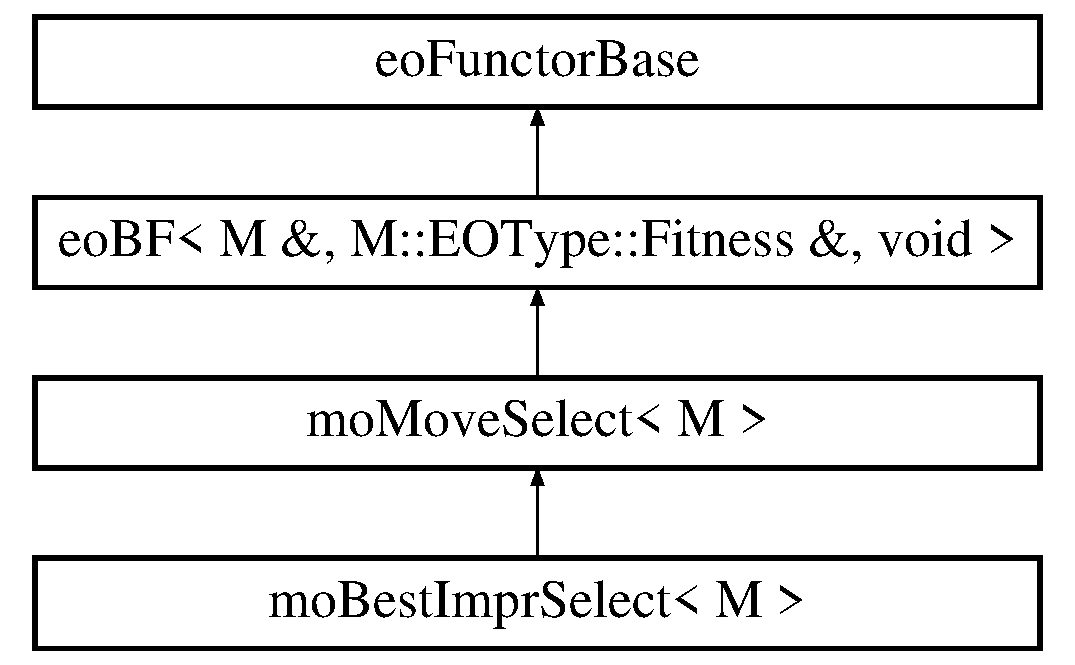
\includegraphics[height=4cm]{classmo_best_impr_select}
\end{center}
\end{figure}
\subsection*{Public Types}
\begin{CompactItemize}
\item 
typedef M::EOType::Fitness {\bf Fitness}\label{classmo_best_impr_select_c4ae17435221fb0a8e8acd285210cfcb}

\begin{CompactList}\small\item\em Alias for the fitness. \item\end{CompactList}\end{CompactItemize}
\subsection*{Public Member Functions}
\begin{CompactItemize}
\item 
void {\bf init} (const {\bf Fitness} \&\_\-fitness)
\begin{CompactList}\small\item\em Procedure which initialise the exploration. \item\end{CompactList}\item 
bool {\bf update} (const M \&\_\-move, const {\bf Fitness} \&\_\-fitness)
\begin{CompactList}\small\item\em {\bf Function} that indicates if the current move has not improved the fitness. \item\end{CompactList}\item 
void {\bf operator()} (M \&\_\-move, {\bf Fitness} \&\_\-fitness)
\begin{CompactList}\small\item\em Procedure which saved the best move and fitness. \item\end{CompactList}\end{CompactItemize}
\subsection*{Private Attributes}
\begin{CompactItemize}
\item 
bool {\bf first\_\-time}\label{classmo_best_impr_select_352b14d206b0772eb9f40efb7beb0f13}

\begin{CompactList}\small\item\em Allowing to know if at least one move has been generated. \item\end{CompactList}\item 
M {\bf best\_\-move}\label{classmo_best_impr_select_bd86f70519f954c07ff0d8a2a3a8ff6a}

\begin{CompactList}\small\item\em The best move. \item\end{CompactList}\item 
{\bf Fitness} {\bf best\_\-fitness}\label{classmo_best_impr_select_e51345fe28ca7cbaca65bdad1aa8ecb7}

\begin{CompactList}\small\item\em The best fitness. \item\end{CompactList}\end{CompactItemize}


\subsection{Detailed Description}
\subsubsection*{template$<$class M$>$ class moBestImprSelect$<$ M $>$}

One of the possible \doxyref{moMoveSelect}{p.}{classmo_move_select}. 

All neighbors are considered, and the movement which enables the best improvement is selected. 

Definition at line 47 of file moBestImprSelect.h.

\subsection{Member Function Documentation}
\index{moBestImprSelect@{moBestImprSelect}!init@{init}}
\index{init@{init}!moBestImprSelect@{moBestImprSelect}}
\subsubsection{\setlength{\rightskip}{0pt plus 5cm}template$<$class M$>$ void {\bf moBestImprSelect}$<$ M $>$::init (const {\bf Fitness} \& {\em \_\-fitness})\hspace{0.3cm}{\tt  [inline, virtual]}}\label{classmo_best_impr_select_83f961549986b8ad94692e433aa79114}


Procedure which initialise the exploration. 

\begin{Desc}
\item[Parameters:]
\begin{description}
\item[{\em \_\-fitness}]The current fitness. \end{description}
\end{Desc}


Implements {\bf moMoveSelect$<$ M $>$} \doxyref{}{p.}{classmo_move_select_58038bd859632c1bd022d23d9792bdca}.

Definition at line 58 of file moBestImprSelect.h.

References moBestImprSelect$<$ M $>$::first\_\-time.\index{moBestImprSelect@{moBestImprSelect}!update@{update}}
\index{update@{update}!moBestImprSelect@{moBestImprSelect}}
\subsubsection{\setlength{\rightskip}{0pt plus 5cm}template$<$class M$>$ bool {\bf moBestImprSelect}$<$ M $>$::update (const M \& {\em \_\-move}, const {\bf Fitness} \& {\em \_\-fitness})\hspace{0.3cm}{\tt  [inline, virtual]}}\label{classmo_best_impr_select_5c0729fd316b0ef78406bce5ca91de2a}


{\bf Function} that indicates if the current move has not improved the fitness. 

If the given fitness enables an improvment, the move (\doxyref{moMove}{p.}{classmo_move}) and the fitness linked to this move are saved.

\begin{Desc}
\item[Parameters:]
\begin{description}
\item[{\em \_\-move}]a move. \item[{\em \_\-fitness}]a fitness linked to the move. \end{description}
\end{Desc}
\begin{Desc}
\item[Returns:]TRUE if the move does not improve the fitness. \end{Desc}


Implements {\bf moMoveSelect$<$ M $>$} \doxyref{}{p.}{classmo_move_select_5b4d3b2f030cca80c563c3db0c4af404}.

Definition at line 76 of file moBestImprSelect.h.

References moBestImprSelect$<$ M $>$::best\_\-fitness, moBestImprSelect$<$ M $>$::best\_\-move, and moBestImprSelect$<$ M $>$::first\_\-time.\index{moBestImprSelect@{moBestImprSelect}!operator()@{operator()}}
\index{operator()@{operator()}!moBestImprSelect@{moBestImprSelect}}
\subsubsection{\setlength{\rightskip}{0pt plus 5cm}template$<$class M$>$ void {\bf moBestImprSelect}$<$ M $>$::operator() (M \& {\em \_\-move}, {\bf Fitness} \& {\em \_\-fitness})\hspace{0.3cm}{\tt  [inline, virtual]}}\label{classmo_best_impr_select_33b3de7bd322f737eb97cce9a5404527}


Procedure which saved the best move and fitness. 

\begin{Desc}
\item[Parameters:]
\begin{description}
\item[{\em \_\-move}]the current move (result of the procedure). \item[{\em \_\-fitness}]the current fitness (result of the procedure). \end{description}
\end{Desc}


Implements {\bf eoBF$<$ M \&, M::EOType::Fitness \&, void $>$}.

Definition at line 94 of file moBestImprSelect.h.

References moBestImprSelect$<$ M $>$::best\_\-fitness, moBestImprSelect$<$ M $>$::best\_\-move, and moBestImprSelect$<$ M $>$::first\_\-time.

The documentation for this class was generated from the following file:\begin{CompactItemize}
\item 
moBestImprSelect.h\end{CompactItemize}

\section{mo\-Comparator$<$ EOT $>$ Class Template Reference}
\label{classmo_comparator}\index{moComparator@{moComparator}}
Template for classes which need to compare two EOT and indicate if the first is \char`\"{}better\char`\"{} than the second.  


{\tt \#include $<$mo\-Comparator.h$>$}

Inheritance diagram for mo\-Comparator$<$ EOT $>$::\begin{figure}[H]
\begin{center}
\leavevmode
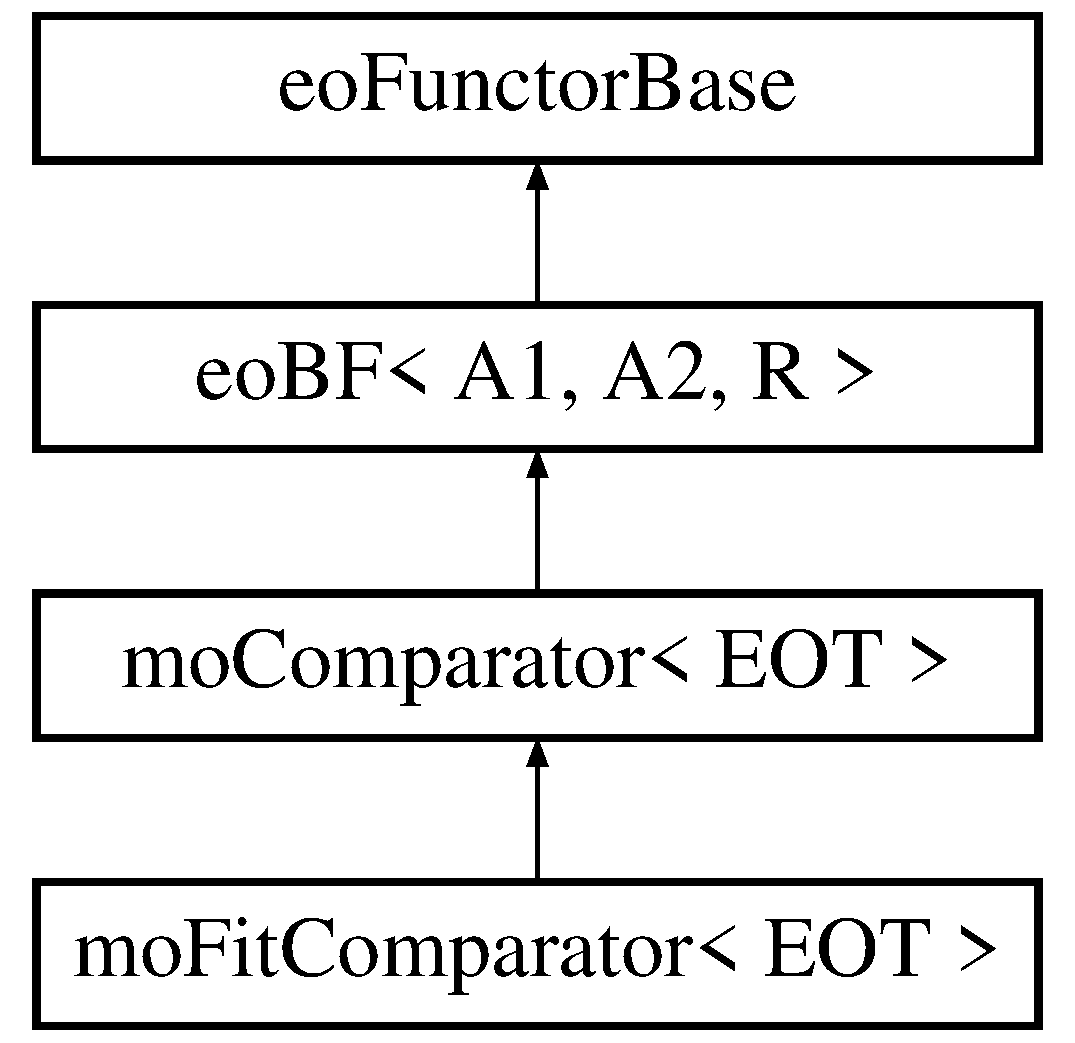
\includegraphics[height=4cm]{classmo_comparator}
\end{center}
\end{figure}


\subsection{Detailed Description}
\subsubsection*{template$<$class EOT$>$ class mo\-Comparator$<$ EOT $>$}

Template for classes which need to compare two EOT and indicate if the first is \char`\"{}better\char`\"{} than the second. 

The objects that extend this template describe how an EOT is \char`\"{}better\char`\"{} than an other. 



Definition at line 45 of file mo\-Comparator.h.

The documentation for this class was generated from the following file:\begin{CompactItemize}
\item 
mo\-Comparator.h\end{CompactItemize}

\section{mo\-Cooling\-Schedule Class Reference}
\label{classmo_cooling_schedule}\index{moCoolingSchedule@{moCoolingSchedule}}
This class gives the description of a cooling schedule.  


{\tt \#include $<$mo\-Cooling\-Schedule.h$>$}

Inheritance diagram for mo\-Cooling\-Schedule::\begin{figure}[H]
\begin{center}
\leavevmode
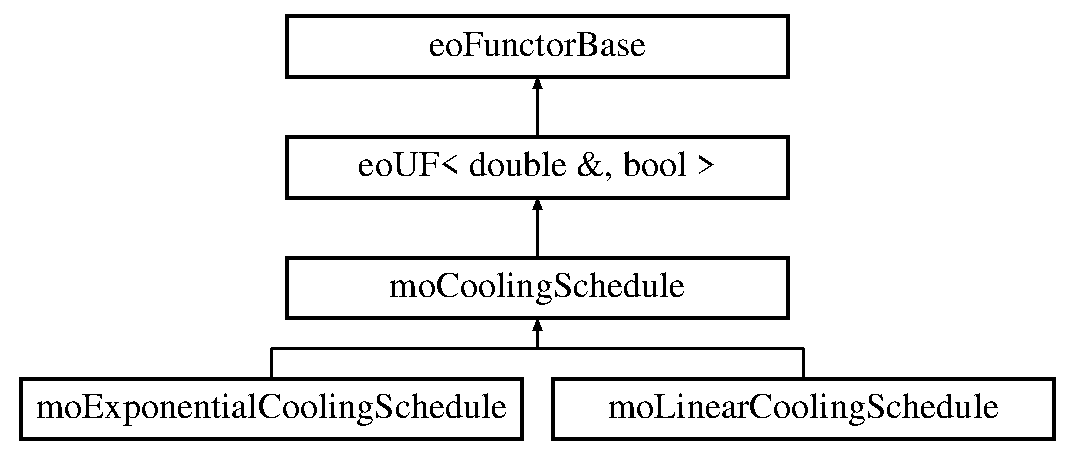
\includegraphics[height=4cm]{classmo_cooling_schedule}
\end{center}
\end{figure}


\subsection{Detailed Description}
This class gives the description of a cooling schedule. 

It is only a description... An object that herits from this class is needed to be used in a {\bf mo\-SA}{\rm (p.\,\pageref{classmo_s_a})}. See {\bf mo\-Exponential\-Cooling\-Schedule}{\rm (p.\,\pageref{classmo_exponential_cooling_schedule})} or {\bf mo\-Linear\-Cooling\-Schedule}{\rm (p.\,\pageref{classmo_linear_cooling_schedule})} for example. 



Definition at line 46 of file mo\-Cooling\-Schedule.h.

The documentation for this class was generated from the following file:\begin{CompactItemize}
\item 
mo\-Cooling\-Schedule.h\end{CompactItemize}

\section{mo\-Exponential\-Cooling\-Schedule Class Reference}
\label{classmo_exponential_cooling_schedule}\index{moExponentialCoolingSchedule@{moExponentialCoolingSchedule}}
One of the possible {\bf mo\-Cooling\-Schedule}{\rm (p.\,\pageref{classmo_cooling_schedule})}.  


{\tt \#include $<$mo\-Exponential\-Cooling\-Schedule.h$>$}

Inheritance diagram for mo\-Exponential\-Cooling\-Schedule::\begin{figure}[H]
\begin{center}
\leavevmode
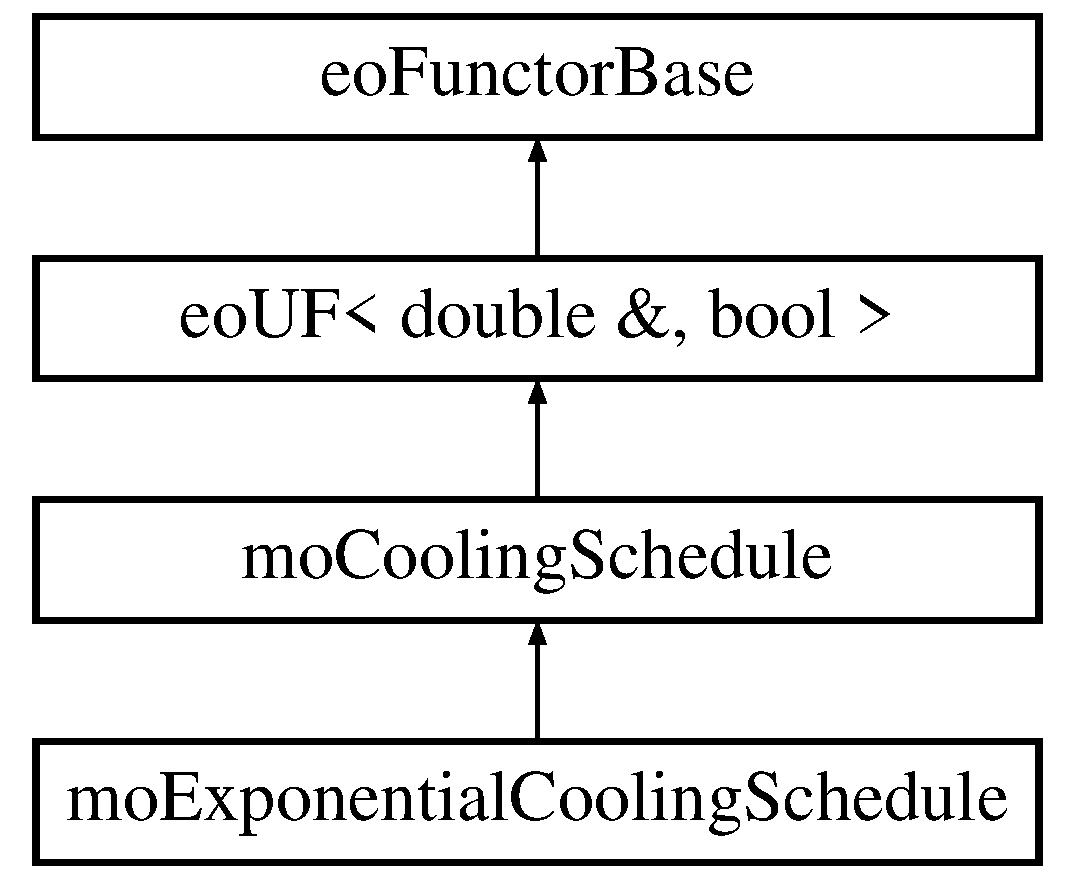
\includegraphics[height=4cm]{classmo_exponential_cooling_schedule}
\end{center}
\end{figure}
\subsection*{Public Member Functions}
\begin{CompactItemize}
\item 
{\bf mo\-Exponential\-Cooling\-Schedule} (double \_\-threshold, double \_\-ratio)
\begin{CompactList}\small\item\em Simple constructor. \item\end{CompactList}\item 
bool {\bf operator()} (double \&\_\-temperature)
\begin{CompactList}\small\item\em Function which proceeds to the cooling. \item\end{CompactList}\end{CompactItemize}
\subsection*{Private Attributes}
\begin{CompactItemize}
\item 
double {\bf threshold}\label{classmo_exponential_cooling_schedule_r0}

\begin{CompactList}\small\item\em The temperature threhold. \item\end{CompactList}\item 
double {\bf ratio}\label{classmo_exponential_cooling_schedule_r1}

\begin{CompactList}\small\item\em The decreasing factor of the temperature. \item\end{CompactList}\end{CompactItemize}


\subsection{Detailed Description}
One of the possible {\bf mo\-Cooling\-Schedule}{\rm (p.\,\pageref{classmo_cooling_schedule})}. 

An other very simple cooling schedule, the temperature decrease according to a ratio while the temperature is greater than a given threshold. 



Definition at line 46 of file mo\-Exponential\-Cooling\-Schedule.h.

\subsection{Constructor \& Destructor Documentation}
\index{moExponentialCoolingSchedule@{mo\-Exponential\-Cooling\-Schedule}!moExponentialCoolingSchedule@{moExponentialCoolingSchedule}}
\index{moExponentialCoolingSchedule@{moExponentialCoolingSchedule}!moExponentialCoolingSchedule@{mo\-Exponential\-Cooling\-Schedule}}
\subsubsection{\setlength{\rightskip}{0pt plus 5cm}mo\-Exponential\-Cooling\-Schedule::mo\-Exponential\-Cooling\-Schedule (double {\em \_\-threshold}, double {\em \_\-ratio})\hspace{0.3cm}{\tt  [inline]}}\label{classmo_exponential_cooling_schedule_a0}


Simple constructor. 

\begin{Desc}
\item[Parameters:]
\begin{description}
\item[{\em \_\-threshold}]the threshold. \item[{\em \_\-ratio}]the ratio used to descrease the temperature. \end{description}
\end{Desc}


Definition at line 55 of file mo\-Exponential\-Cooling\-Schedule.h.

References ratio, and threshold.

\subsection{Member Function Documentation}
\index{moExponentialCoolingSchedule@{mo\-Exponential\-Cooling\-Schedule}!operator()@{operator()}}
\index{operator()@{operator()}!moExponentialCoolingSchedule@{mo\-Exponential\-Cooling\-Schedule}}
\subsubsection{\setlength{\rightskip}{0pt plus 5cm}bool mo\-Exponential\-Cooling\-Schedule::operator() (double \& {\em \_\-temperature})\hspace{0.3cm}{\tt  [inline, virtual]}}\label{classmo_exponential_cooling_schedule_a1}


Function which proceeds to the cooling. 

It decreases the temperature and indicates if it is greater than the threshold.

\begin{Desc}
\item[Parameters:]
\begin{description}
\item[{\em \_\-temperature}]the current temperature. \end{description}
\end{Desc}
\begin{Desc}
\item[Returns:]if the new temperature (current temperature $\ast$ ratio) is greater than the threshold. \end{Desc}


Implements {\bf eo\-UF$<$ double \&, bool $>$}.

Definition at line 65 of file mo\-Exponential\-Cooling\-Schedule.h.

The documentation for this class was generated from the following file:\begin{CompactItemize}
\item 
mo\-Exponential\-Cooling\-Schedule.h\end{CompactItemize}

\section{mo\-First\-Impr\-Select$<$ M $>$ Class Template Reference}
\label{classmo_first_impr_select}\index{moFirstImprSelect@{moFirstImprSelect}}
One possible {\bf mo\-Move\-Select}{\rm (p.\,\pageref{classmo_move_select})}.  


{\tt \#include $<$mo\-First\-Impr\-Select.h$>$}

Inheritance diagram for mo\-First\-Impr\-Select$<$ M $>$::\begin{figure}[H]
\begin{center}
\leavevmode
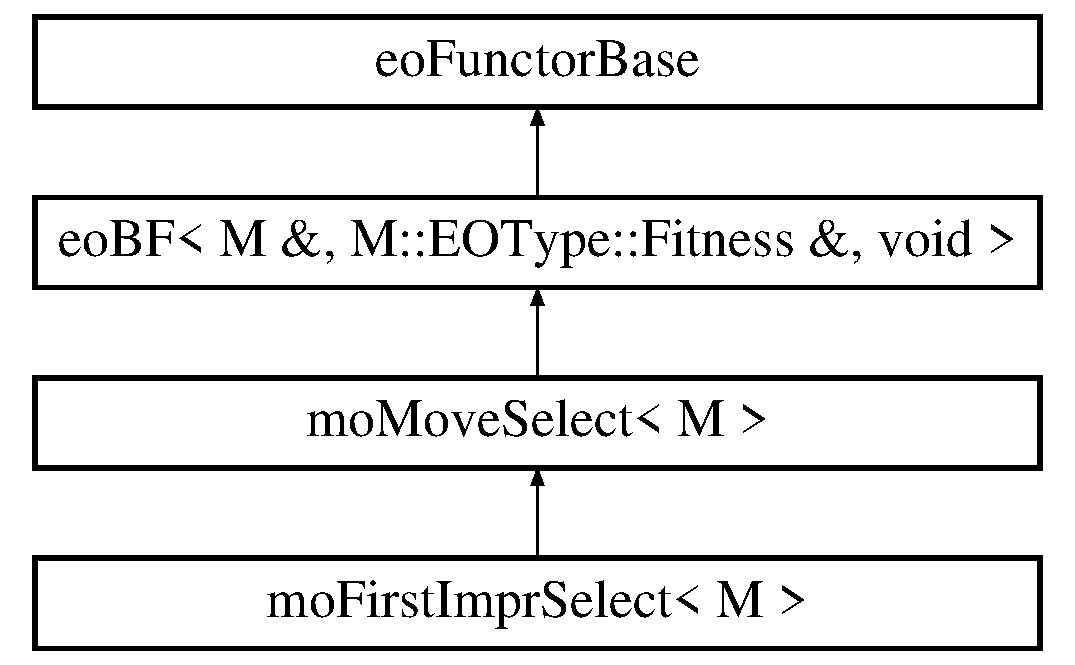
\includegraphics[height=4cm]{classmo_first_impr_select}
\end{center}
\end{figure}
\subsection*{Public Types}
\begin{CompactItemize}
\item 
typedef M::EOType::Fitness {\bf Fitness}\label{classmo_first_impr_select_w0}

\begin{CompactList}\small\item\em Alias for the fitness. \item\end{CompactList}\end{CompactItemize}
\subsection*{Public Member Functions}
\begin{CompactItemize}
\item 
virtual void {\bf init} (const {\bf Fitness} \&\_\-fitness)
\begin{CompactList}\small\item\em Procedure which initialise the exploration. \item\end{CompactList}\item 
bool {\bf update} (const M \&\_\-move, const {\bf Fitness} \&\_\-fitness)
\begin{CompactList}\small\item\em Function that indicates if the current move has not improved the fitness. \item\end{CompactList}\item 
void {\bf operator()} (M \&\_\-move, {\bf Fitness} \&\_\-fitness)
\begin{CompactList}\small\item\em Procedure which saved the best move and fitness. \item\end{CompactList}\end{CompactItemize}
\subsection*{Private Attributes}
\begin{CompactItemize}
\item 
bool {\bf valid}\label{classmo_first_impr_select_r0}

\begin{CompactList}\small\item\em Allow to know if at least one move has improved the solution. \item\end{CompactList}\item 
M {\bf best\_\-move}\label{classmo_first_impr_select_r1}

\begin{CompactList}\small\item\em Best stored movement. \item\end{CompactList}\item 
{\bf Fitness} {\bf initial\_\-fitness}\label{classmo_first_impr_select_r2}

\begin{CompactList}\small\item\em Initial fitness. \item\end{CompactList}\item 
{\bf Fitness} {\bf best\_\-fitness}\label{classmo_first_impr_select_r3}

\begin{CompactList}\small\item\em Best stored fitness. \item\end{CompactList}\end{CompactItemize}


\subsection{Detailed Description}
\subsubsection*{template$<$class M$>$ class mo\-First\-Impr\-Select$<$ M $>$}

One possible {\bf mo\-Move\-Select}{\rm (p.\,\pageref{classmo_move_select})}. 

The neighborhood is explored until a move enables an improvment of the current solution. 



Definition at line 48 of file mo\-First\-Impr\-Select.h.

\subsection{Member Function Documentation}
\index{moFirstImprSelect@{mo\-First\-Impr\-Select}!init@{init}}
\index{init@{init}!moFirstImprSelect@{mo\-First\-Impr\-Select}}
\subsubsection{\setlength{\rightskip}{0pt plus 5cm}template$<$class M$>$ virtual void {\bf mo\-First\-Impr\-Select}$<$ M $>$::init (const {\bf Fitness} \& {\em \_\-fitness})\hspace{0.3cm}{\tt  [inline, virtual]}}\label{classmo_first_impr_select_a0}


Procedure which initialise the exploration. 

It save the current fitness as the initial value for the fitness. \begin{Desc}
\item[Parameters:]
\begin{description}
\item[{\em \_\-fitness}]The current fitness. \end{description}
\end{Desc}


Implements {\bf mo\-Move\-Select$<$ M $>$} {\rm (p.\,\pageref{classmo_move_select_a0})}.

Definition at line 60 of file mo\-First\-Impr\-Select.h.

References mo\-First\-Impr\-Select$<$ M $>$::initial\_\-fitness, and mo\-First\-Impr\-Select$<$ M $>$::valid.\index{moFirstImprSelect@{mo\-First\-Impr\-Select}!update@{update}}
\index{update@{update}!moFirstImprSelect@{mo\-First\-Impr\-Select}}
\subsubsection{\setlength{\rightskip}{0pt plus 5cm}template$<$class M$>$ bool {\bf mo\-First\-Impr\-Select}$<$ M $>$::update (const M \& {\em \_\-move}, const {\bf Fitness} \& {\em \_\-fitness})\hspace{0.3cm}{\tt  [inline, virtual]}}\label{classmo_first_impr_select_a1}


Function that indicates if the current move has not improved the fitness. 

If the given fitness enables an improvment, the move ({\bf mo\-Move}{\rm (p.\,\pageref{classmo_move})}) should be applied to the current solution.

\begin{Desc}
\item[Parameters:]
\begin{description}
\item[{\em \_\-move}]a move. \item[{\em \_\-fitness}]a fitness linked to the move. \end{description}
\end{Desc}
\begin{Desc}
\item[Returns:]true if the move does not improve the fitness. \end{Desc}


Implements {\bf mo\-Move\-Select$<$ M $>$} {\rm (p.\,\pageref{classmo_move_select_a1})}.

Definition at line 75 of file mo\-First\-Impr\-Select.h.

References mo\-First\-Impr\-Select$<$ M $>$::best\_\-fitness, mo\-First\-Impr\-Select$<$ M $>$::best\_\-move, and mo\-First\-Impr\-Select$<$ M $>$::valid.\index{moFirstImprSelect@{mo\-First\-Impr\-Select}!operator()@{operator()}}
\index{operator()@{operator()}!moFirstImprSelect@{mo\-First\-Impr\-Select}}
\subsubsection{\setlength{\rightskip}{0pt plus 5cm}template$<$class M$>$ void {\bf mo\-First\-Impr\-Select}$<$ M $>$::operator() (M \& {\em \_\-move}, {\bf Fitness} \& {\em \_\-fitness})\hspace{0.3cm}{\tt  [inline]}}\label{classmo_first_impr_select_a2}


Procedure which saved the best move and fitness. 

\begin{Desc}
\item[Parameters:]
\begin{description}
\item[{\em \_\-move}]the current move (result of the procedure). \item[{\em \_\-fitness}]the current fitness (result of the procedure). \end{description}
\end{Desc}


Definition at line 96 of file mo\-First\-Impr\-Select.h.

The documentation for this class was generated from the following file:\begin{CompactItemize}
\item 
mo\-First\-Impr\-Select.h\end{CompactItemize}

\section{mo\-Fit\-Comparator$<$ EOT $>$ Class Template Reference}
\label{classmo_fit_comparator}\index{moFitComparator@{moFitComparator}}
Comparison according to the fitness.  


{\tt \#include $<$mo\-Fit\-Comparator.h$>$}

Inheritance diagram for mo\-Fit\-Comparator$<$ EOT $>$::\begin{figure}[H]
\begin{center}
\leavevmode
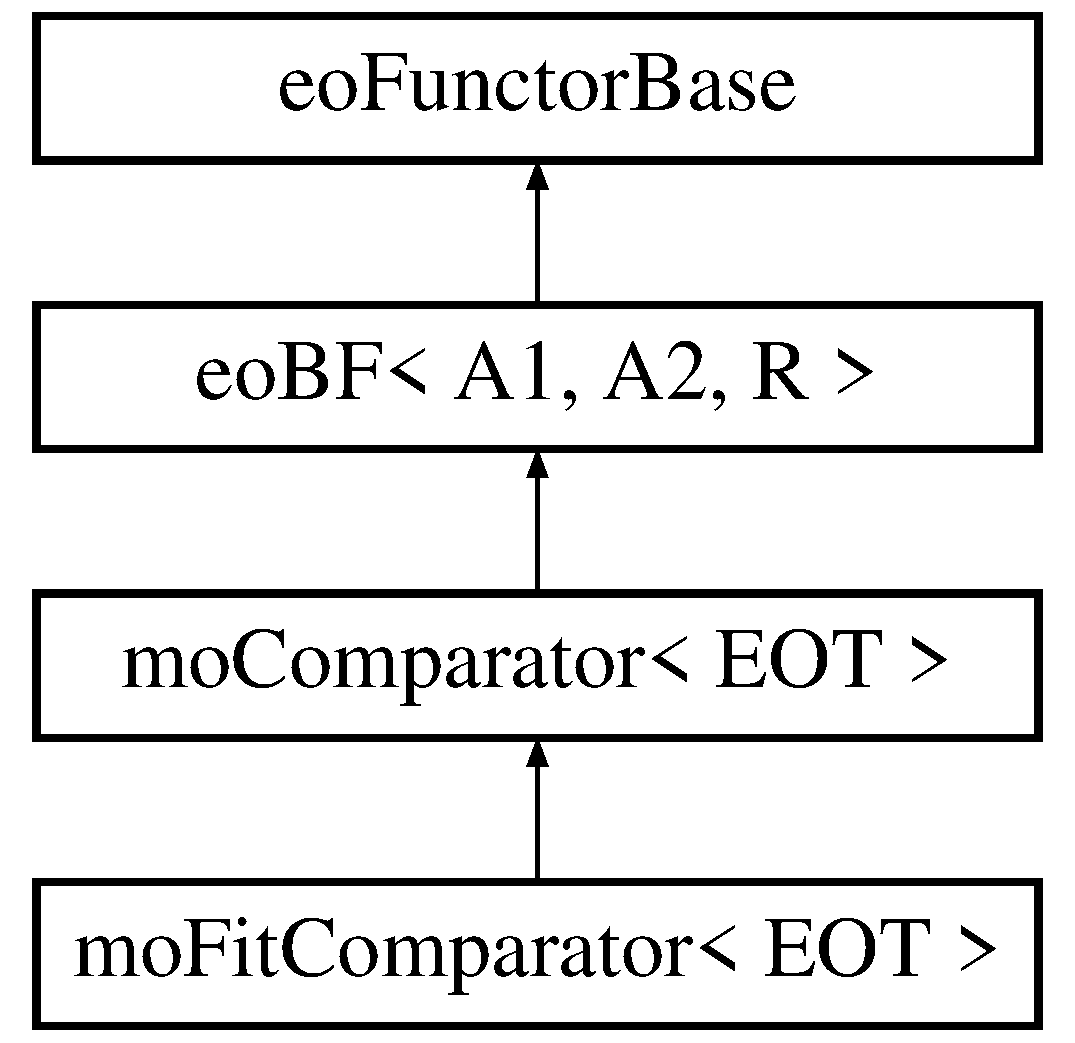
\includegraphics[height=2cm]{classmo_fit_comparator}
\end{center}
\end{figure}
\subsection*{Public Member Functions}
\begin{CompactItemize}
\item 
bool \bf{operator()} (const EOT \&\_\-solution1, const EOT \&\_\-solution2)
\begin{CompactList}\small\item\em Function which makes the comparison and gives the result. \item\end{CompactList}\end{CompactItemize}


\subsection{Detailed Description}
\subsubsection*{template$<$class EOT$>$ class mo\-Fit\-Comparator$<$ EOT $>$}

Comparison according to the fitness. 

An EOT is better than an other if its fitness is better. 



Definition at line 46 of file mo\-Fit\-Comparator.h.

\subsection{Member Function Documentation}
\index{moFitComparator@{mo\-Fit\-Comparator}!operator()@{operator()}}
\index{operator()@{operator()}!moFitComparator@{mo\-Fit\-Comparator}}
\subsubsection{\setlength{\rightskip}{0pt plus 5cm}template$<$class EOT$>$ bool \bf{mo\-Fit\-Comparator}$<$ EOT $>$::operator() (const EOT \& {\em \_\-solution1}, const EOT \& {\em \_\-solution2})\hspace{0.3cm}{\tt  [inline]}}\label{classmo_fit_comparator_c920d5a49deb16710daf1e5fcde6b16c}


Function which makes the comparison and gives the result. 

\begin{Desc}
\item[Parameters:]
\begin{description}
\item[{\em \_\-solution1}]The first solution. \item[{\em \_\-solution2}]The second solution. \end{description}
\end{Desc}
\begin{Desc}
\item[Returns:]true if the fitness of the first solution is better than the second solution, false else. \end{Desc}


Definition at line 56 of file mo\-Fit\-Comparator.h.

The documentation for this class was generated from the following file:\begin{CompactItemize}
\item 
mo\-Fit\-Comparator.h\end{CompactItemize}

\section{mo\-Fit\-Sol\-Continue$<$ EOT $>$ Class Template Reference}
\label{classmo_fit_sol_continue}\index{moFitSolContinue@{moFitSolContinue}}
One possible stop criterion for a solution-based heuristic.  


{\tt \#include $<$mo\-Fit\-Sol\-Continue.h$>$}

Inheritance diagram for mo\-Fit\-Sol\-Continue$<$ EOT $>$::\begin{figure}[H]
\begin{center}
\leavevmode
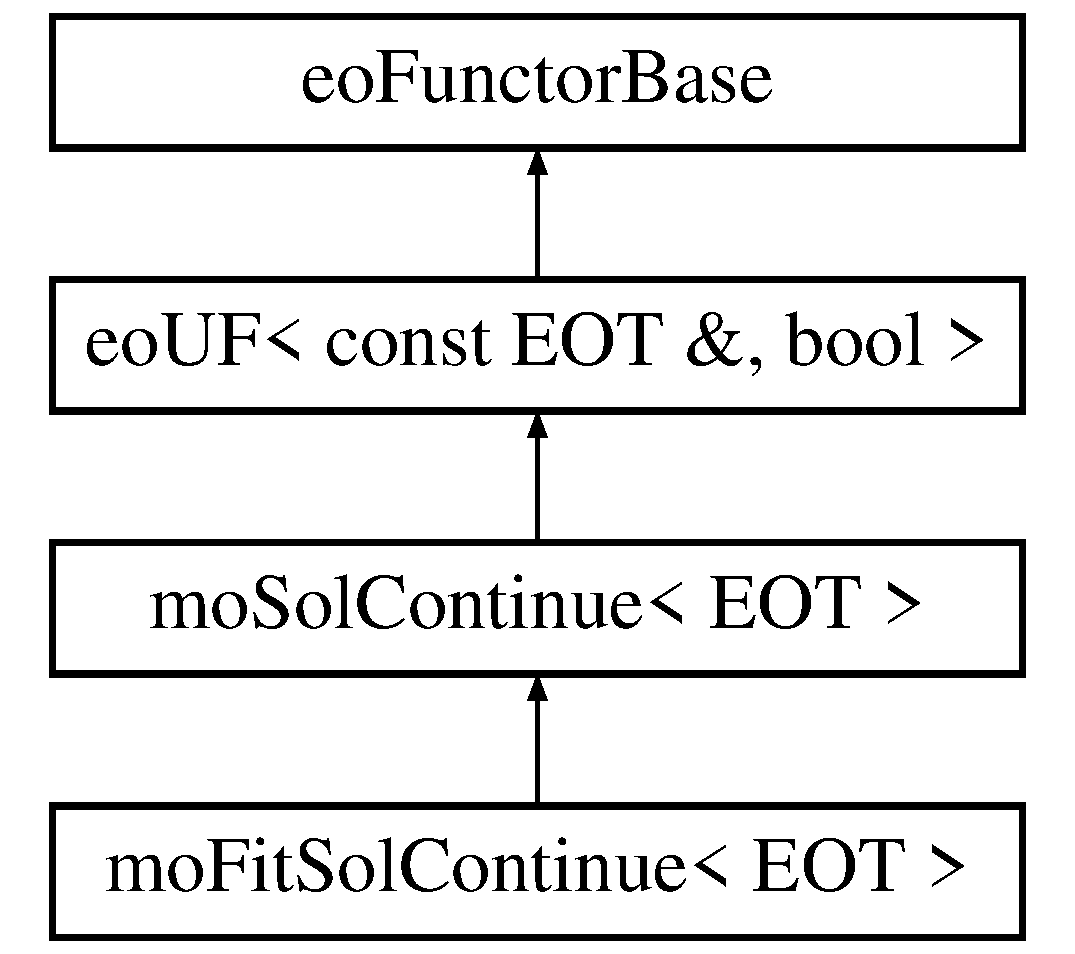
\includegraphics[height=4cm]{classmo_fit_sol_continue}
\end{center}
\end{figure}
\subsection*{Public Types}
\begin{CompactItemize}
\item 
typedef EOT::Fitness {\bf Fitness}\label{classmo_fit_sol_continue_w0}

\begin{CompactList}\small\item\em Alias for the fitness. \item\end{CompactList}\end{CompactItemize}
\subsection*{Public Member Functions}
\begin{CompactItemize}
\item 
{\bf mo\-Fit\-Sol\-Continue} ({\bf Fitness} \_\-fitness)
\begin{CompactList}\small\item\em Basic constructor. \item\end{CompactList}\item 
bool {\bf operator()} (const EOT \&\_\-solution)
\begin{CompactList}\small\item\em Function that activates the stopping criterion. \item\end{CompactList}\item 
void {\bf init} ()
\begin{CompactList}\small\item\em Procedure which allows to initialise all the stuff needed. \item\end{CompactList}\end{CompactItemize}
\subsection*{Private Attributes}
\begin{CompactItemize}
\item 
{\bf Fitness} {\bf fitness}\label{classmo_fit_sol_continue_r0}

\begin{CompactList}\small\item\em Fitness target. \item\end{CompactList}\end{CompactItemize}


\subsection{Detailed Description}
\subsubsection*{template$<$class EOT$>$ class mo\-Fit\-Sol\-Continue$<$ EOT $>$}

One possible stop criterion for a solution-based heuristic. 

The stop criterion corresponds to a fitness threshold gained. 



Definition at line 46 of file mo\-Fit\-Sol\-Continue.h.

\subsection{Constructor \& Destructor Documentation}
\index{moFitSolContinue@{mo\-Fit\-Sol\-Continue}!moFitSolContinue@{moFitSolContinue}}
\index{moFitSolContinue@{moFitSolContinue}!moFitSolContinue@{mo\-Fit\-Sol\-Continue}}
\subsubsection{\setlength{\rightskip}{0pt plus 5cm}template$<$class EOT$>$ {\bf mo\-Fit\-Sol\-Continue}$<$ EOT $>$::{\bf mo\-Fit\-Sol\-Continue} ({\bf Fitness} {\em \_\-fitness})\hspace{0.3cm}{\tt  [inline]}}\label{classmo_fit_sol_continue_a0}


Basic constructor. 

\begin{Desc}
\item[Parameters:]
\begin{description}
\item[{\em \_\-fitness}]The fitness to reach. \end{description}
\end{Desc}


Definition at line 57 of file mo\-Fit\-Sol\-Continue.h.

References mo\-Fit\-Sol\-Continue$<$ EOT $>$::fitness.

\subsection{Member Function Documentation}
\index{moFitSolContinue@{mo\-Fit\-Sol\-Continue}!operator()@{operator()}}
\index{operator()@{operator()}!moFitSolContinue@{mo\-Fit\-Sol\-Continue}}
\subsubsection{\setlength{\rightskip}{0pt plus 5cm}template$<$class EOT$>$ bool {\bf mo\-Fit\-Sol\-Continue}$<$ EOT $>$::operator() (const EOT \& {\em \_\-solution})\hspace{0.3cm}{\tt  [inline, virtual]}}\label{classmo_fit_sol_continue_a1}


Function that activates the stopping criterion. 

Indicates if the fitness threshold has not yet been reached.

\begin{Desc}
\item[Parameters:]
\begin{description}
\item[{\em \_\-solution}]the current solution. \end{description}
\end{Desc}
\begin{Desc}
\item[Returns:]true or false according to the value of the fitness. \end{Desc}


Implements {\bf eo\-UF$<$ const EOT \&, bool $>$}.

Definition at line 67 of file mo\-Fit\-Sol\-Continue.h.

References mo\-Fit\-Sol\-Continue$<$ EOT $>$::fitness.\index{moFitSolContinue@{mo\-Fit\-Sol\-Continue}!init@{init}}
\index{init@{init}!moFitSolContinue@{mo\-Fit\-Sol\-Continue}}
\subsubsection{\setlength{\rightskip}{0pt plus 5cm}template$<$class EOT$>$ void {\bf mo\-Fit\-Sol\-Continue}$<$ EOT $>$::init ()\hspace{0.3cm}{\tt  [inline, virtual]}}\label{classmo_fit_sol_continue_a2}


Procedure which allows to initialise all the stuff needed. 

It can be also used to reinitialize all the needed things. 

Implements {\bf mo\-Sol\-Continue$<$ EOT $>$} {\rm (p.\,\pageref{classmo_sol_continue_a0})}.

Definition at line 81 of file mo\-Fit\-Sol\-Continue.h.

The documentation for this class was generated from the following file:\begin{CompactItemize}
\item 
mo\-Fit\-Sol\-Continue.h\end{CompactItemize}

\section{mo\-Gen\-Sol\-Continue$<$ EOT $>$ Class Template Reference}
\label{classmo_gen_sol_continue}\index{moGenSolContinue@{moGenSolContinue}}
One possible stop criterion for a solution-based heuristic.  


{\tt \#include $<$mo\-Gen\-Sol\-Continue.h$>$}

Inheritance diagram for mo\-Gen\-Sol\-Continue$<$ EOT $>$::\begin{figure}[H]
\begin{center}
\leavevmode
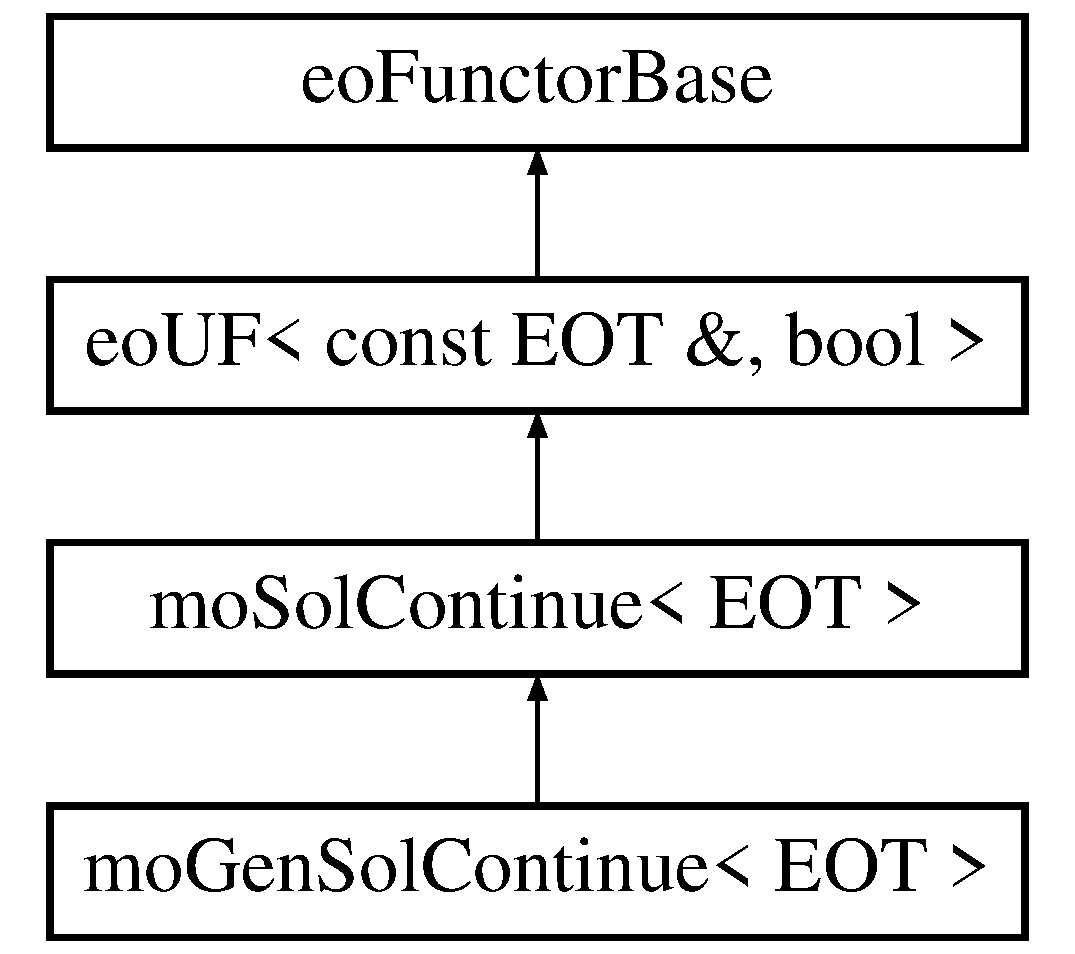
\includegraphics[height=4cm]{classmo_gen_sol_continue}
\end{center}
\end{figure}
\subsection*{Public Member Functions}
\begin{CompactItemize}
\item 
{\bf mo\-Gen\-Sol\-Continue} (unsigned int \_\-generation\-Maximum\-Number)
\begin{CompactList}\small\item\em Simple constructor. \item\end{CompactList}\item 
bool {\bf operator()} (const EOT \&\_\-solution)
\begin{CompactList}\small\item\em Function that activates the stop criterion. \item\end{CompactList}\item 
void {\bf init} ()
\begin{CompactList}\small\item\em Procedure which allows to initialise the generation counter. \item\end{CompactList}\end{CompactItemize}
\subsection*{Private Attributes}
\begin{CompactItemize}
\item 
unsigned int {\bf generation\-Maximum\-Number}\label{classmo_gen_sol_continue_r0}

\begin{CompactList}\small\item\em Iteration maximum number. \item\end{CompactList}\item 
unsigned int {\bf generation\-Number}\label{classmo_gen_sol_continue_r1}

\begin{CompactList}\small\item\em Iteration current number. \item\end{CompactList}\end{CompactItemize}


\subsection{Detailed Description}
\subsubsection*{template$<$class EOT$>$ class mo\-Gen\-Sol\-Continue$<$ EOT $>$}

One possible stop criterion for a solution-based heuristic. 

The stop criterion corresponds to a maximum number of iteration. 



Definition at line 46 of file mo\-Gen\-Sol\-Continue.h.

\subsection{Constructor \& Destructor Documentation}
\index{moGenSolContinue@{mo\-Gen\-Sol\-Continue}!moGenSolContinue@{moGenSolContinue}}
\index{moGenSolContinue@{moGenSolContinue}!moGenSolContinue@{mo\-Gen\-Sol\-Continue}}
\subsubsection{\setlength{\rightskip}{0pt plus 5cm}template$<$class EOT$>$ {\bf mo\-Gen\-Sol\-Continue}$<$ EOT $>$::{\bf mo\-Gen\-Sol\-Continue} (unsigned int {\em \_\-generation\-Maximum\-Number})\hspace{0.3cm}{\tt  [inline]}}\label{classmo_gen_sol_continue_a0}


Simple constructor. 

\begin{Desc}
\item[Parameters:]
\begin{description}
\item[{\em \_\-generation\-Maximum\-Number}]The maximum number of generations. \end{description}
\end{Desc}


Definition at line 54 of file mo\-Gen\-Sol\-Continue.h.

References mo\-Gen\-Sol\-Continue$<$ EOT $>$::generation\-Maximum\-Number, and mo\-Gen\-Sol\-Continue$<$ EOT $>$::generation\-Number.

\subsection{Member Function Documentation}
\index{moGenSolContinue@{mo\-Gen\-Sol\-Continue}!operator()@{operator()}}
\index{operator()@{operator()}!moGenSolContinue@{mo\-Gen\-Sol\-Continue}}
\subsubsection{\setlength{\rightskip}{0pt plus 5cm}template$<$class EOT$>$ bool {\bf mo\-Gen\-Sol\-Continue}$<$ EOT $>$::operator() (const EOT \& {\em \_\-solution})\hspace{0.3cm}{\tt  [inline, virtual]}}\label{classmo_gen_sol_continue_a1}


Function that activates the stop criterion. 

Increments the counter and returns TRUE if the current number of iteration is lower than the given maximum number of iterations.

\begin{Desc}
\item[Parameters:]
\begin{description}
\item[{\em \_\-solution}]The current solution. \end{description}
\end{Desc}
\begin{Desc}
\item[Returns:]true or false according to the current generation number. \end{Desc}


Implements {\bf eo\-UF$<$ const EOT \&, bool $>$}.

Definition at line 66 of file mo\-Gen\-Sol\-Continue.h.

References mo\-Gen\-Sol\-Continue$<$ EOT $>$::generation\-Number.\index{moGenSolContinue@{mo\-Gen\-Sol\-Continue}!init@{init}}
\index{init@{init}!moGenSolContinue@{mo\-Gen\-Sol\-Continue}}
\subsubsection{\setlength{\rightskip}{0pt plus 5cm}template$<$class EOT$>$ void {\bf mo\-Gen\-Sol\-Continue}$<$ EOT $>$::init ()\hspace{0.3cm}{\tt  [inline, virtual]}}\label{classmo_gen_sol_continue_a2}


Procedure which allows to initialise the generation counter. 

It can also be used to reset the iteration counter. 

Implements {\bf mo\-Sol\-Continue$<$ EOT $>$} {\rm (p.\,\pageref{classmo_sol_continue_a0})}.

Definition at line 78 of file mo\-Gen\-Sol\-Continue.h.

References mo\-Gen\-Sol\-Continue$<$ EOT $>$::generation\-Number.

The documentation for this class was generated from the following file:\begin{CompactItemize}
\item 
mo\-Gen\-Sol\-Continue.h\end{CompactItemize}

\section{mo\-HC$<$ M $>$ Class Template Reference}
\label{classmo_h_c}\index{moHC@{moHC}}
Hill Climbing (HC).  


{\tt \#include $<$mo\-HC.h$>$}

Inheritance diagram for mo\-HC$<$ M $>$::\begin{figure}[H]
\begin{center}
\leavevmode
\includegraphics[height=5cm]{classmo_h_c}
\end{center}
\end{figure}
\subsection*{Public Member Functions}
\begin{CompactItemize}
\item 
{\bf mo\-HC} ({\bf mo\-Move\-Init}$<$ M $>$ \&\_\-move\_\-initializer, {\bf mo\-Next\-Move}$<$ M $>$ \&\_\-next\_\-move\_\-generator, {\bf mo\-Move\-Incr\-Eval}$<$ M $>$ \&\_\-incremental\_\-evaluation, {\bf mo\-Move\-Select}$<$ M $>$ \&\_\-move\_\-selection, {\bf eo\-Eval\-Func}$<$ {\bf EOT} $>$ \&\_\-full\_\-evaluation)
\begin{CompactList}\small\item\em Full constructor. \item\end{CompactList}\item 
{\bf mo\-HC} ({\bf mo\-Move\-Expl}$<$ M $>$ \&\_\-move\_\-explorer, {\bf eo\-Eval\-Func}$<$ {\bf EOT} $>$ \&\_\-full\_\-evaluation)
\begin{CompactList}\small\item\em Light constructor. \item\end{CompactList}\item 
bool {\bf operator()} ({\bf EOT} \&\_\-solution)
\begin{CompactList}\small\item\em Function which launches the HC. \item\end{CompactList}\end{CompactItemize}
\subsection*{Private Types}
\begin{CompactItemize}
\item 
typedef M::EOType {\bf EOT}\label{classmo_h_c_y0}

\begin{CompactList}\small\item\em Alias for the type. \item\end{CompactList}\item 
typedef EOT::Fitness {\bf Fitness}\label{classmo_h_c_y1}

\begin{CompactList}\small\item\em Alias for the fitness. \item\end{CompactList}\end{CompactItemize}
\subsection*{Private Attributes}
\begin{CompactItemize}
\item 
{\bf mo\-Move\-Expl}$<$ M $>$ \& {\bf move\_\-explorer}\label{classmo_h_c_r0}

\begin{CompactList}\small\item\em Complete exploration of the neighborhood. \item\end{CompactList}\item 
{\bf eo\-Eval\-Func}$<$ {\bf EOT} $>$ \& {\bf full\_\-evaluation}\label{classmo_h_c_r1}

\begin{CompactList}\small\item\em A full evaluation function. \item\end{CompactList}\end{CompactItemize}


\subsection{Detailed Description}
\subsubsection*{template$<$class M$>$ class mo\-HC$<$ M $>$}

Hill Climbing (HC). 

Class which describes the algorithm for a hill climbing. 



Definition at line 49 of file mo\-HC.h.

\subsection{Constructor \& Destructor Documentation}
\index{moHC@{mo\-HC}!moHC@{moHC}}
\index{moHC@{moHC}!moHC@{mo\-HC}}
\subsubsection{\setlength{\rightskip}{0pt plus 5cm}template$<$class M$>$ {\bf mo\-HC}$<$ M $>$::{\bf mo\-HC} ({\bf mo\-Move\-Init}$<$ M $>$ \& {\em \_\-move\_\-initializer}, {\bf mo\-Next\-Move}$<$ M $>$ \& {\em \_\-next\_\-move\_\-generator}, {\bf mo\-Move\-Incr\-Eval}$<$ M $>$ \& {\em \_\-incremental\_\-evaluation}, {\bf mo\-Move\-Select}$<$ M $>$ \& {\em \_\-move\_\-selection}, {\bf eo\-Eval\-Func}$<$ {\bf EOT} $>$ \& {\em \_\-full\_\-evaluation})\hspace{0.3cm}{\tt  [inline]}}\label{classmo_h_c_a0}


Full constructor. 

All the boxes are given in order the HC to use a {\bf mo\-HCMove\-Loop\-Expl}{\rm (p.\,\pageref{classmo_h_c_move_loop_expl})}.

\begin{Desc}
\item[Parameters:]
\begin{description}
\item[{\em \_\-move\_\-initializer}]a move initialiser. \item[{\em \_\-next\_\-move\_\-generator}]a neighborhood explorer. \item[{\em \_\-incremental\_\-evaluation}]a (generally) efficient evaluation function. \item[{\em \_\-move\_\-selection}]a move selector. \item[{\em \_\-full\_\-evaluation}]a full evaluation function. \end{description}
\end{Desc}


Definition at line 69 of file mo\-HC.h.

References mo\-HC$<$ M $>$::full\_\-evaluation, and mo\-HC$<$ M $>$::move\_\-explorer.\index{moHC@{mo\-HC}!moHC@{moHC}}
\index{moHC@{moHC}!moHC@{mo\-HC}}
\subsubsection{\setlength{\rightskip}{0pt plus 5cm}template$<$class M$>$ {\bf mo\-HC}$<$ M $>$::{\bf mo\-HC} ({\bf mo\-Move\-Expl}$<$ M $>$ \& {\em \_\-move\_\-explorer}, {\bf eo\-Eval\-Func}$<$ {\bf EOT} $>$ \& {\em \_\-full\_\-evaluation})\hspace{0.3cm}{\tt  [inline]}}\label{classmo_h_c_a1}


Light constructor. 

This constructor allow to use another {\bf mo\-Move\-Expl}{\rm (p.\,\pageref{classmo_move_expl})} (generally not a {\bf mo\-HCMove\-Loop\-Expl}{\rm (p.\,\pageref{classmo_h_c_move_loop_expl})}).

\begin{Desc}
\item[Parameters:]
\begin{description}
\item[{\em \_\-move\_\-explorer}]a complete explorer. \item[{\em \_\-full\_\-evaluation}]a full evaluation function. \end{description}
\end{Desc}


Definition at line 82 of file mo\-HC.h.

References mo\-HC$<$ M $>$::full\_\-evaluation, and mo\-HC$<$ M $>$::move\_\-explorer.

\subsection{Member Function Documentation}
\index{moHC@{mo\-HC}!operator()@{operator()}}
\index{operator()@{operator()}!moHC@{mo\-HC}}
\subsubsection{\setlength{\rightskip}{0pt plus 5cm}template$<$class M$>$ bool {\bf mo\-HC}$<$ M $>$::operator() ({\bf EOT} \& {\em \_\-solution})\hspace{0.3cm}{\tt  [inline]}}\label{classmo_h_c_a2}


Function which launches the HC. 

The HC has to improve a current solution. As the {\bf mo\-SA}{\rm (p.\,\pageref{classmo_s_a})} and the mo TS, it can be used for HYBRIDATION in an evolutionnary algorithm.

\begin{Desc}
\item[Parameters:]
\begin{description}
\item[{\em \_\-solution}]a current solution to improve. \end{description}
\end{Desc}
\begin{Desc}
\item[Returns:]true. \end{Desc}


Definition at line 94 of file mo\-HC.h.

References mo\-HC$<$ M $>$::EOT, mo\-HC$<$ M $>$::full\_\-evaluation, and mo\-HC$<$ M $>$::move\_\-explorer.

The documentation for this class was generated from the following file:\begin{CompactItemize}
\item 
mo\-HC.h\end{CompactItemize}

\section{moHCMoveLoopExpl$<$ M $>$ Class Template Reference}
\label{classmo_h_c_move_loop_expl}\index{moHCMoveLoopExpl@{moHCMoveLoopExpl}}
Iterative explorer used by a \doxyref{moHC}{p.}{classmo_h_c}.  


{\tt \#include $<$moHCMoveLoopExpl.h$>$}

Inheritance diagram for moHCMoveLoopExpl$<$ M $>$::\begin{figure}[H]
\begin{center}
\leavevmode
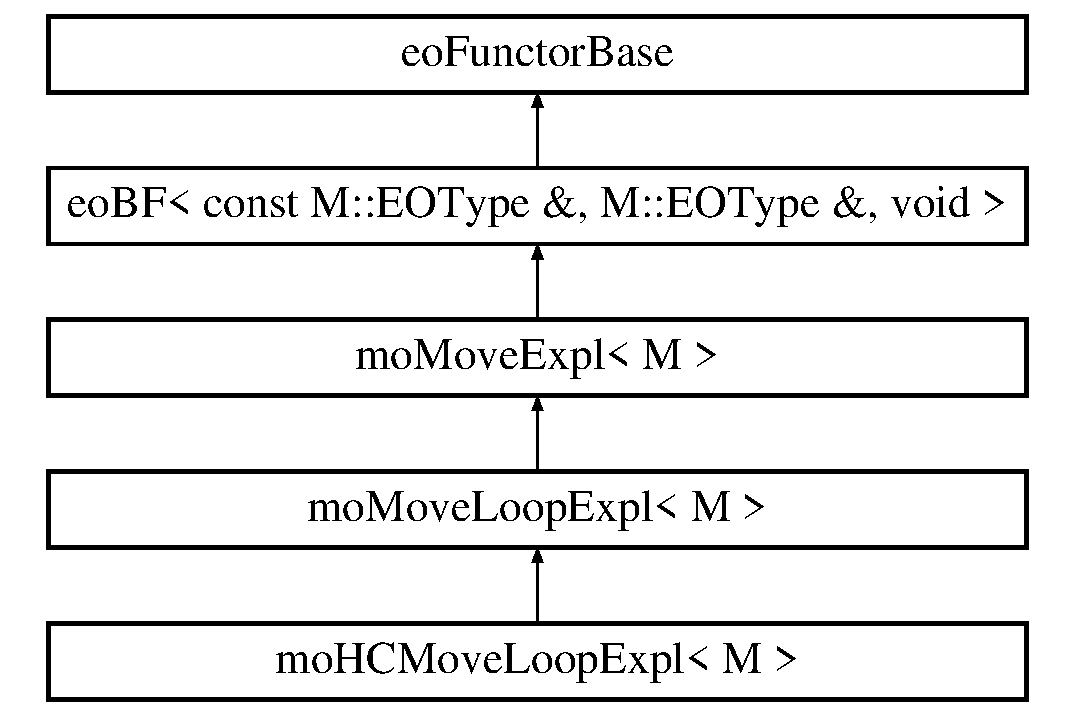
\includegraphics[height=5cm]{classmo_h_c_move_loop_expl}
\end{center}
\end{figure}
\subsection*{Public Member Functions}
\begin{CompactItemize}
\item 
{\bf moHCMoveLoopExpl} ({\bf moMoveInit}$<$ M $>$ \&\_\-move\_\-initializer, {\bf moNextMove}$<$ M $>$ \&\_\-next\_\-move\_\-generator, {\bf moMoveIncrEval}$<$ M $>$ \&\_\-incremental\_\-evaluation, {\bf moMoveSelect}$<$ M $>$ \&\_\-move\_\-selection)
\begin{CompactList}\small\item\em Constructor. \item\end{CompactList}\item 
void {\bf operator()} (const {\bf EOT} \&\_\-old\_\-solution, {\bf EOT} \&\_\-new\_\-solution)
\begin{CompactList}\small\item\em Procedure which launches the explorer. \item\end{CompactList}\end{CompactItemize}
\subsection*{Private Types}
\begin{CompactItemize}
\item 
typedef M::EOType {\bf EOT}\label{classmo_h_c_move_loop_expl_077befd4106c201eafd3ea22bcea2fe9}

\begin{CompactList}\small\item\em Alias for the type. \item\end{CompactList}\item 
typedef M::EOType::Fitness {\bf Fitness}\label{classmo_h_c_move_loop_expl_f24871224316d5549b9013a2d27ab465}

\begin{CompactList}\small\item\em Alias for the fitness. \item\end{CompactList}\end{CompactItemize}
\subsection*{Private Attributes}
\begin{CompactItemize}
\item 
{\bf moMoveInit}$<$ M $>$ \& {\bf move\_\-initializer}\label{classmo_h_c_move_loop_expl_17506f3f1172714f9adbfa4e8a15953a}

\begin{CompactList}\small\item\em Move initialiser. \item\end{CompactList}\item 
{\bf moNextMove}$<$ M $>$ \& {\bf next\_\-move\_\-generator}\label{classmo_h_c_move_loop_expl_fdc44d40d8859bae1d7b92e77f36aa30}

\begin{CompactList}\small\item\em Neighborhood explorer. \item\end{CompactList}\item 
{\bf moMoveIncrEval}$<$ M $>$ \& {\bf incremental\_\-evaluation}\label{classmo_h_c_move_loop_expl_a044b28f972d007a22736b646d86f265}

\begin{CompactList}\small\item\em (generally) Efficient evaluation. \item\end{CompactList}\item 
{\bf moMoveSelect}$<$ M $>$ \& {\bf move\_\-selection}\label{classmo_h_c_move_loop_expl_5f0532e0ee8ef8ecaeeb4e56342be443}

\begin{CompactList}\small\item\em Move selector. \item\end{CompactList}\end{CompactItemize}


\subsection{Detailed Description}
\subsubsection*{template$<$class M$>$ class moHCMoveLoopExpl$<$ M $>$}

Iterative explorer used by a \doxyref{moHC}{p.}{classmo_h_c}. 

Definition at line 47 of file moHCMoveLoopExpl.h.

\subsection{Constructor \& Destructor Documentation}
\index{moHCMoveLoopExpl@{moHCMoveLoopExpl}!moHCMoveLoopExpl@{moHCMoveLoopExpl}}
\index{moHCMoveLoopExpl@{moHCMoveLoopExpl}!moHCMoveLoopExpl@{moHCMoveLoopExpl}}
\subsubsection{\setlength{\rightskip}{0pt plus 5cm}template$<$class M$>$ {\bf moHCMoveLoopExpl}$<$ M $>$::{\bf moHCMoveLoopExpl} ({\bf moMoveInit}$<$ M $>$ \& {\em \_\-move\_\-initializer}, {\bf moNextMove}$<$ M $>$ \& {\em \_\-next\_\-move\_\-generator}, {\bf moMoveIncrEval}$<$ M $>$ \& {\em \_\-incremental\_\-evaluation}, {\bf moMoveSelect}$<$ M $>$ \& {\em \_\-move\_\-selection})\hspace{0.3cm}{\tt  [inline]}}\label{classmo_h_c_move_loop_expl_fac2eb6695ba1b797ffab4f290d760b8}


Constructor. 

All the boxes have to be specified.

\begin{Desc}
\item[Parameters:]
\begin{description}
\item[{\em \_\-move\_\-initializer}]The move initialiser. \item[{\em \_\-next\_\-move\_\-generator}]The neighbourhood explorer. \item[{\em \_\-incremental\_\-evaluation}](generally) Efficient evaluation function. \item[{\em \_\-move\_\-selection}]The move selector. \end{description}
\end{Desc}


Definition at line 66 of file moHCMoveLoopExpl.h.

\subsection{Member Function Documentation}
\index{moHCMoveLoopExpl@{moHCMoveLoopExpl}!operator()@{operator()}}
\index{operator()@{operator()}!moHCMoveLoopExpl@{moHCMoveLoopExpl}}
\subsubsection{\setlength{\rightskip}{0pt plus 5cm}template$<$class M$>$ void {\bf moHCMoveLoopExpl}$<$ M $>$::operator() (const {\bf EOT} \& {\em \_\-old\_\-solution}, {\bf EOT} \& {\em \_\-new\_\-solution})\hspace{0.3cm}{\tt  [inline, virtual]}}\label{classmo_h_c_move_loop_expl_fe9362c10d74a5e6ed09b56345396192}


Procedure which launches the explorer. 

The exploration starts from an old solution and provides a new solution.

\begin{Desc}
\item[Parameters:]
\begin{description}
\item[{\em \_\-old\_\-solution}]The current solution. \item[{\em \_\-new\_\-solution}]The new solution (result of the procedure). \end{description}
\end{Desc}


Implements {\bf eoBF$<$ const M::EOType \&, M::EOType \&, void $>$}.

Definition at line 79 of file moHCMoveLoopExpl.h.

References moHCMoveLoopExpl$<$ M $>$::incremental\_\-evaluation, moHCMoveLoopExpl$<$ M $>$::move\_\-initializer, moHCMoveLoopExpl$<$ M $>$::move\_\-selection, and moHCMoveLoopExpl$<$ M $>$::next\_\-move\_\-generator.

The documentation for this class was generated from the following file:\begin{CompactItemize}
\item 
moHCMoveLoopExpl.h\end{CompactItemize}

\section{mo\-ILS$<$ M $>$ Class Template Reference}
\label{classmo_i_l_s}\index{moILS@{moILS}}
Iterated Local Search (ILS).  


{\tt \#include $<$mo\-ILS.h$>$}

\subsection*{Public Member Functions}
\begin{CompactItemize}
\item 
\bf{mo\-ILS} (\bf{mo\-Algo}$<$ \bf{EOT} $>$ \&\_\-algorithm, \bf{mo\-Sol\-Continue}$<$ \bf{EOT} $>$ \&\_\-continue, \bf{mo\-Comparator}$<$ \bf{EOT} $>$ \&\_\-acceptance\_\-criterion, \bf{eo\-Mon\-Op}$<$ \bf{EOT} $>$ \&\_\-perturbation, \bf{eo\-Eval\-Func}$<$ \bf{EOT} $>$ \&\_\-full\_\-evaluation)
\begin{CompactList}\small\item\em Generic constructor. \item\end{CompactList}\item 
\bf{mo\-ILS} (\bf{mo\-Move\-Init}$<$ M $>$ \&\_\-move\_\-initializer, \bf{mo\-Next\-Move}$<$ M $>$ \&\_\-next\_\-move\_\-generator, \bf{mo\-Move\-Incr\-Eval}$<$ M $>$ \&\_\-incremental\_\-evaluation, \bf{mo\-Move\-Select}$<$ M $>$ \&\_\-move\_\-selection, \bf{mo\-Sol\-Continue}$<$ \bf{EOT} $>$ \&\_\-continue, \bf{mo\-Comparator}$<$ \bf{EOT} $>$ \&\_\-acceptance\_\-criterion, \bf{eo\-Mon\-Op}$<$ \bf{EOT} $>$ \&\_\-perturbation, \bf{eo\-Eval\-Func}$<$ \bf{EOT} $>$ \&\_\-full\_\-evaluation)
\begin{CompactList}\small\item\em Constructor for using a \doxyref{mo\-HC}{p.}{classmo_h_c} for the \doxyref{mo\-Algo}{p.}{classmo_algo}. \item\end{CompactList}\item 
\bf{mo\-ILS} (\bf{mo\-Move\-Init}$<$ M $>$ \&\_\-move\_\-initializer, \bf{mo\-Next\-Move}$<$ M $>$ \&\_\-next\_\-move\_\-generator, \bf{mo\-Move\-Incr\-Eval}$<$ M $>$ \&\_\-incremental\_\-evaluation, \bf{mo\-Tabu\-List}$<$ M $>$ \&\_\-tabu\_\-list, \bf{mo\-Aspir\-Crit}$<$ M $>$ \&\_\-aspiration\_\-criterion, \bf{mo\-Sol\-Continue}$<$ \bf{EOT} $>$ \&\_\-mo\-TS\_\-continue, \bf{mo\-Sol\-Continue}$<$ \bf{EOT} $>$ \&\_\-continue, \bf{mo\-Comparator}$<$ \bf{EOT} $>$ \&\_\-acceptance\_\-criterion, \bf{eo\-Mon\-Op}$<$ \bf{EOT} $>$ \&\_\-perturbation, \bf{eo\-Eval\-Func}$<$ \bf{EOT} $>$ \&\_\-full\_\-evaluation)
\begin{CompactList}\small\item\em Constructor for using a \doxyref{mo\-TS}{p.}{classmo_t_s} for the \doxyref{mo\-Algo}{p.}{classmo_algo}. \item\end{CompactList}\item 
\bf{mo\-ILS} (\bf{mo\-Rand\-Move}$<$ M $>$ \&\_\-random\_\-move\_\-generator, \bf{mo\-Move\-Incr\-Eval}$<$ M $>$ \&\_\-incremental\_\-evaluation, \bf{mo\-Sol\-Continue}$<$ \bf{EOT} $>$ \&\_\-mo\-SA\_\-continue, double \_\-initial\_\-temperature, \bf{mo\-Cooling\-Schedule} \&\_\-cooling\_\-schedule, \bf{mo\-Sol\-Continue}$<$ \bf{EOT} $>$ \&\_\-continue, \bf{mo\-Comparator}$<$ \bf{EOT} $>$ \&\_\-acceptance\_\-criterion, \bf{eo\-Mon\-Op}$<$ \bf{EOT} $>$ \&\_\-perturbation, \bf{eo\-Eval\-Func}$<$ \bf{EOT} $>$ \&\_\-full\_\-evaluation)
\begin{CompactList}\small\item\em Constructor for using a \doxyref{mo\-SA}{p.}{classmo_s_a} for the \doxyref{mo\-Algo}{p.}{classmo_algo}. \item\end{CompactList}\item 
bool \bf{operator()} (\bf{EOT} \&\_\-solution)
\begin{CompactList}\small\item\em \doxyref{Function} which launches the ILS. \item\end{CompactList}\end{CompactItemize}
\subsection*{Private Types}
\begin{CompactItemize}
\item 
typedef M::EOType \bf{EOT}\label{classmo_i_l_s_c81bafc611e4d4fd44347cf7162198c7}

\begin{CompactList}\small\item\em Alias for the type. \item\end{CompactList}\item 
typedef EOT::Fitness \bf{Fitness}\label{classmo_i_l_s_8c464a9eae064a78eff75d4c722b619c}

\begin{CompactList}\small\item\em Alias for the fitness. \item\end{CompactList}\end{CompactItemize}
\subsection*{Private Attributes}
\begin{CompactItemize}
\item 
\bf{mo\-Algo}$<$ \bf{EOT} $>$ \& \bf{algorithm}\label{classmo_i_l_s_5651a4d94b59d523d341d5d6e24ca311}

\begin{CompactList}\small\item\em The solution based heuristic. \item\end{CompactList}\item 
\bf{mo\-Sol\-Continue}$<$ \bf{EOT} $>$ \& \bf{continu}\label{classmo_i_l_s_30edab439401d7ec04fd8d37b4513d94}

\begin{CompactList}\small\item\em The stopping criterion. \item\end{CompactList}\item 
\bf{mo\-Comparator}$<$ \bf{EOT} $>$ \& \bf{acceptance\_\-criterion}\label{classmo_i_l_s_295f6d0342c67bd3dc4cb82e2adc26be}

\begin{CompactList}\small\item\em The acceptance criterion. \item\end{CompactList}\item 
\bf{eo\-Mon\-Op}$<$ \bf{EOT} $>$ \& \bf{perturbation}\label{classmo_i_l_s_f667a1bda06b6d221292df9aba3db8a2}

\begin{CompactList}\small\item\em The perturbation generator. \item\end{CompactList}\item 
\bf{eo\-Eval\-Func}$<$ \bf{EOT} $>$ \& \bf{full\_\-evaluation}\label{classmo_i_l_s_8e8c383ac6ec34aaf071fa18bb54be67}

\begin{CompactList}\small\item\em The full evaluation function. \item\end{CompactList}\end{CompactItemize}


\subsection{Detailed Description}
\subsubsection*{template$<$class M$>$ class mo\-ILS$<$ M $>$}

Iterated Local Search (ILS). 

Class which describes the algorithm for a iterated local search. 



Definition at line 50 of file mo\-ILS.h.

\subsection{Constructor \& Destructor Documentation}
\index{moILS@{mo\-ILS}!moILS@{moILS}}
\index{moILS@{moILS}!moILS@{mo\-ILS}}
\subsubsection{\setlength{\rightskip}{0pt plus 5cm}template$<$class M$>$ \bf{mo\-ILS}$<$ M $>$::\bf{mo\-ILS} (\bf{mo\-Algo}$<$ \bf{EOT} $>$ \& {\em \_\-algorithm}, \bf{mo\-Sol\-Continue}$<$ \bf{EOT} $>$ \& {\em \_\-continue}, \bf{mo\-Comparator}$<$ \bf{EOT} $>$ \& {\em \_\-acceptance\_\-criterion}, \bf{eo\-Mon\-Op}$<$ \bf{EOT} $>$ \& {\em \_\-perturbation}, \bf{eo\-Eval\-Func}$<$ \bf{EOT} $>$ \& {\em \_\-full\_\-evaluation})\hspace{0.3cm}{\tt  [inline]}}\label{classmo_i_l_s_c83f81ba0836ae262305efa15eeb3da2}


Generic constructor. 

Generic constructor using a \doxyref{mo\-Algo}{p.}{classmo_algo}

\begin{Desc}
\item[Parameters:]
\begin{description}
\item[{\em \_\-algorithm}]The solution based heuristic to use. \item[{\em \_\-continue}]The stopping criterion. \item[{\em \_\-acceptance\_\-criterion}]The acceptance criterion. \item[{\em \_\-perturbation}]The pertubation generator. \item[{\em \_\-full\_\-evaluation}]The evaluation function. \end{description}
\end{Desc}


Definition at line 70 of file mo\-ILS.h.\index{moILS@{mo\-ILS}!moILS@{moILS}}
\index{moILS@{moILS}!moILS@{mo\-ILS}}
\subsubsection{\setlength{\rightskip}{0pt plus 5cm}template$<$class M$>$ \bf{mo\-ILS}$<$ M $>$::\bf{mo\-ILS} (\bf{mo\-Move\-Init}$<$ M $>$ \& {\em \_\-move\_\-initializer}, \bf{mo\-Next\-Move}$<$ M $>$ \& {\em \_\-next\_\-move\_\-generator}, \bf{mo\-Move\-Incr\-Eval}$<$ M $>$ \& {\em \_\-incremental\_\-evaluation}, \bf{mo\-Move\-Select}$<$ M $>$ \& {\em \_\-move\_\-selection}, \bf{mo\-Sol\-Continue}$<$ \bf{EOT} $>$ \& {\em \_\-continue}, \bf{mo\-Comparator}$<$ \bf{EOT} $>$ \& {\em \_\-acceptance\_\-criterion}, \bf{eo\-Mon\-Op}$<$ \bf{EOT} $>$ \& {\em \_\-perturbation}, \bf{eo\-Eval\-Func}$<$ \bf{EOT} $>$ \& {\em \_\-full\_\-evaluation})\hspace{0.3cm}{\tt  [inline]}}\label{classmo_i_l_s_6d684a1d13ad224a911c8b0277812297}


Constructor for using a \doxyref{mo\-HC}{p.}{classmo_h_c} for the \doxyref{mo\-Algo}{p.}{classmo_algo}. 

\begin{Desc}
\item[Parameters:]
\begin{description}
\item[{\em \_\-move\_\-initializer}]The move initialisation (for the \doxyref{mo\-HC}{p.}{classmo_h_c}). \item[{\em \_\-next\_\-move\_\-generator}]The move generator (for the \doxyref{mo\-HC}{p.}{classmo_h_c}). \item[{\em \_\-incremental\_\-evaluation}]The partial evaluation function (for the \doxyref{mo\-HC}{p.}{classmo_h_c}). \item[{\em \_\-move\_\-selection}]The move selection strategy (for the \doxyref{mo\-HC}{p.}{classmo_h_c}). \item[{\em \_\-continue}]The stopping criterion. \item[{\em \_\-acceptance\_\-criterion}]The acceptance criterion. \item[{\em \_\-perturbation}]The pertubation generator. \item[{\em \_\-full\_\-evaluation}]The evaluation function. \end{description}
\end{Desc}


Definition at line 87 of file mo\-ILS.h.\index{moILS@{mo\-ILS}!moILS@{moILS}}
\index{moILS@{moILS}!moILS@{mo\-ILS}}
\subsubsection{\setlength{\rightskip}{0pt plus 5cm}template$<$class M$>$ \bf{mo\-ILS}$<$ M $>$::\bf{mo\-ILS} (\bf{mo\-Move\-Init}$<$ M $>$ \& {\em \_\-move\_\-initializer}, \bf{mo\-Next\-Move}$<$ M $>$ \& {\em \_\-next\_\-move\_\-generator}, \bf{mo\-Move\-Incr\-Eval}$<$ M $>$ \& {\em \_\-incremental\_\-evaluation}, \bf{mo\-Tabu\-List}$<$ M $>$ \& {\em \_\-tabu\_\-list}, \bf{mo\-Aspir\-Crit}$<$ M $>$ \& {\em \_\-aspiration\_\-criterion}, \bf{mo\-Sol\-Continue}$<$ \bf{EOT} $>$ \& {\em \_\-mo\-TS\_\-continue}, \bf{mo\-Sol\-Continue}$<$ \bf{EOT} $>$ \& {\em \_\-continue}, \bf{mo\-Comparator}$<$ \bf{EOT} $>$ \& {\em \_\-acceptance\_\-criterion}, \bf{eo\-Mon\-Op}$<$ \bf{EOT} $>$ \& {\em \_\-perturbation}, \bf{eo\-Eval\-Func}$<$ \bf{EOT} $>$ \& {\em \_\-full\_\-evaluation})\hspace{0.3cm}{\tt  [inline]}}\label{classmo_i_l_s_740ac81a0d06eb471592ba0861d3a6d7}


Constructor for using a \doxyref{mo\-TS}{p.}{classmo_t_s} for the \doxyref{mo\-Algo}{p.}{classmo_algo}. 

\begin{Desc}
\item[Parameters:]
\begin{description}
\item[{\em \_\-move\_\-initializer}]The move initialisation (for the \doxyref{mo\-TS}{p.}{classmo_t_s}). \item[{\em \_\-next\_\-move\_\-generator}]The move generator (for the \doxyref{mo\-TS}{p.}{classmo_t_s}). \item[{\em \_\-incremental\_\-evaluation}]The partial evaluation function (for the \doxyref{mo\-TS}{p.}{classmo_t_s}). \item[{\em \_\-tabu\_\-list}]The tabu list (for the \doxyref{mo\-TS}{p.}{classmo_t_s} !!!!). \item[{\em \_\-aspiration\_\-criterion}]The aspiration criterion (for the \doxyref{mo\-TS}{p.}{classmo_t_s}). \item[{\em \_\-mo\-TS\_\-continue}]The stopping criterion (for the \doxyref{mo\-TS}{p.}{classmo_t_s}). \item[{\em \_\-continue}]The stopping criterion. \item[{\em \_\-acceptance\_\-criterion}]The acceptance criterion. \item[{\em \_\-perturbation}]The pertubation generator. \item[{\em \_\-full\_\-evaluation}]The evaluation function. \end{description}
\end{Desc}


Definition at line 108 of file mo\-ILS.h.\index{moILS@{mo\-ILS}!moILS@{moILS}}
\index{moILS@{moILS}!moILS@{mo\-ILS}}
\subsubsection{\setlength{\rightskip}{0pt plus 5cm}template$<$class M$>$ \bf{mo\-ILS}$<$ M $>$::\bf{mo\-ILS} (\bf{mo\-Rand\-Move}$<$ M $>$ \& {\em \_\-random\_\-move\_\-generator}, \bf{mo\-Move\-Incr\-Eval}$<$ M $>$ \& {\em \_\-incremental\_\-evaluation}, \bf{mo\-Sol\-Continue}$<$ \bf{EOT} $>$ \& {\em \_\-mo\-SA\_\-continue}, double {\em \_\-initial\_\-temperature}, \bf{mo\-Cooling\-Schedule} \& {\em \_\-cooling\_\-schedule}, \bf{mo\-Sol\-Continue}$<$ \bf{EOT} $>$ \& {\em \_\-continue}, \bf{mo\-Comparator}$<$ \bf{EOT} $>$ \& {\em \_\-acceptance\_\-criterion}, \bf{eo\-Mon\-Op}$<$ \bf{EOT} $>$ \& {\em \_\-perturbation}, \bf{eo\-Eval\-Func}$<$ \bf{EOT} $>$ \& {\em \_\-full\_\-evaluation})\hspace{0.3cm}{\tt  [inline]}}\label{classmo_i_l_s_36bab16abf36957dac36c467b86385bc}


Constructor for using a \doxyref{mo\-SA}{p.}{classmo_s_a} for the \doxyref{mo\-Algo}{p.}{classmo_algo}. 

\begin{Desc}
\item[Parameters:]
\begin{description}
\item[{\em \_\-random\_\-move\_\-generator}]The random move generator (for the \doxyref{mo\-SA}{p.}{classmo_s_a}). \item[{\em \_\-incremental\_\-evaluation}]The partial evaluation function (for the \doxyref{mo\-SA}{p.}{classmo_s_a}). \item[{\em \_\-mo\-SA\_\-continue}]The stopping criterion (for the \doxyref{mo\-SA}{p.}{classmo_s_a}). \item[{\em \_\-initial\_\-temperature}]The initial temperature (for the \doxyref{mo\-SA}{p.}{classmo_s_a}). \item[{\em \_\-cooling\_\-schedule}]The cooling schedule (for the \doxyref{mo\-SA}{p.}{classmo_s_a}). \item[{\em \_\-continue}]The stopping criterion. \item[{\em \_\-acceptance\_\-criterion}]The acceptance criterion. \item[{\em \_\-perturbation}]The pertubation generator. \item[{\em \_\-full\_\-evaluation}]The evaluation function. \end{description}
\end{Desc}


Definition at line 130 of file mo\-ILS.h.

\subsection{Member Function Documentation}
\index{moILS@{mo\-ILS}!operator()@{operator()}}
\index{operator()@{operator()}!moILS@{mo\-ILS}}
\subsubsection{\setlength{\rightskip}{0pt plus 5cm}template$<$class M$>$ bool \bf{mo\-ILS}$<$ M $>$::operator() (\bf{EOT} \& {\em \_\-solution})\hspace{0.3cm}{\tt  [inline, virtual]}}\label{classmo_i_l_s_3f6b950e5a6c363f04b8d4c259502488}


\doxyref{Function} which launches the ILS. 

The ILS has to improve a current solution. As the \doxyref{mo\-SA}{p.}{classmo_s_a}, the \doxyref{mo\-TS}{p.}{classmo_t_s} and the \doxyref{mo\-HC}{p.}{classmo_h_c}, it can be used for HYBRIDATION in an evolutionnary algorithm.

\begin{Desc}
\item[Parameters:]
\begin{description}
\item[{\em \_\-solution}]a current solution to improve. \end{description}
\end{Desc}
\begin{Desc}
\item[Returns:]true. \end{Desc}


Implements \bf{eo\-UF$<$ M::EOType \&, bool $>$}.

Definition at line 146 of file mo\-ILS.h.

References mo\-ILS$<$ M $>$::acceptance\_\-criterion, mo\-ILS$<$ M $>$::algorithm, mo\-ILS$<$ M $>$::continu, mo\-ILS$<$ M $>$::full\_\-evaluation, and mo\-ILS$<$ M $>$::perturbation.

The documentation for this class was generated from the following file:\begin{CompactItemize}
\item 
mo\-ILS.h\end{CompactItemize}

\section{mo\-Impr\-Best\-Fit\-Aspir\-Crit$<$ M $>$ Class Template Reference}
\label{classmo_impr_best_fit_aspir_crit}\index{moImprBestFitAspirCrit@{moImprBestFitAspirCrit}}
One of the possible \doxyref{mo\-Aspir\-Crit}{p.}{classmo_aspir_crit}.  


{\tt \#include $<$mo\-Impr\-Best\-Fit\-Aspir\-Crit.h$>$}

Inheritance diagram for mo\-Impr\-Best\-Fit\-Aspir\-Crit$<$ M $>$::\begin{figure}[H]
\begin{center}
\leavevmode
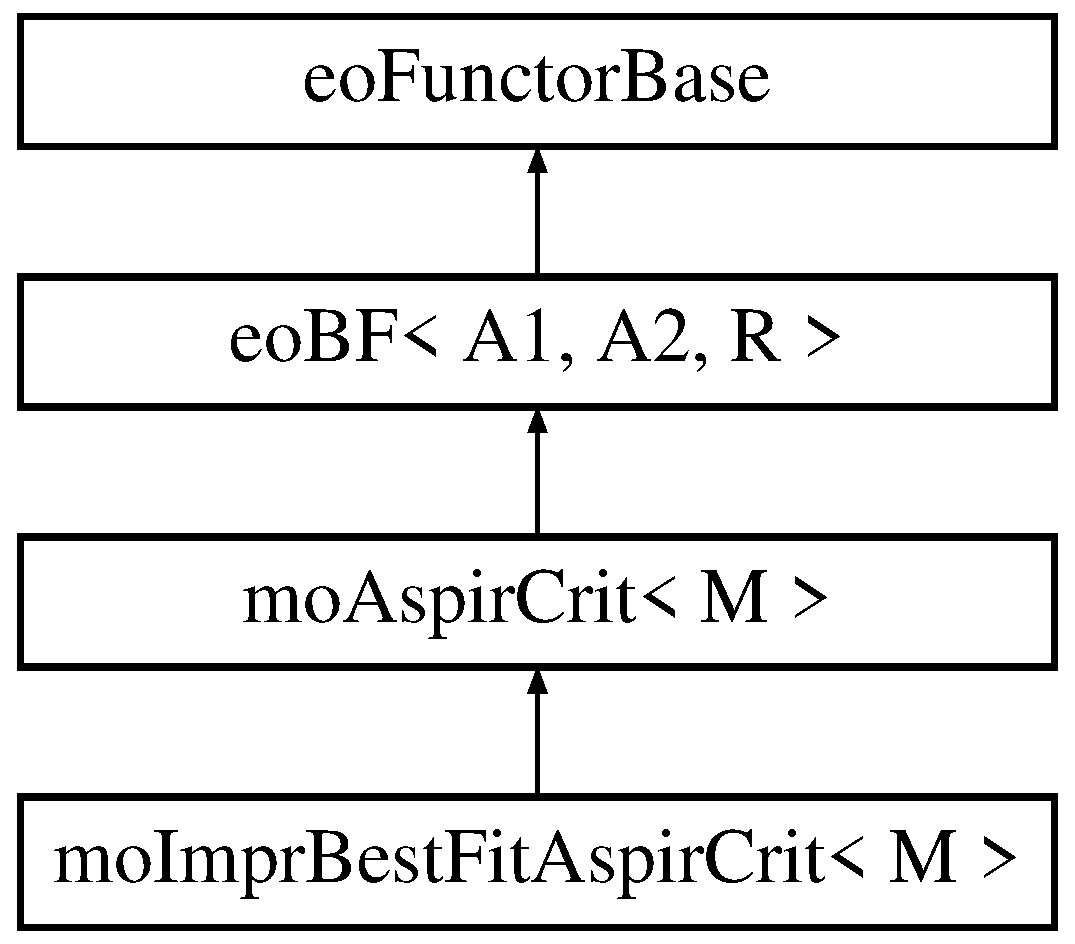
\includegraphics[height=4cm]{classmo_impr_best_fit_aspir_crit}
\end{center}
\end{figure}
\subsection*{Public Types}
\begin{CompactItemize}
\item 
typedef M::EOType::Fitness \bf{Fitness}\label{classmo_impr_best_fit_aspir_crit_0bc1a8c9af99781e662570c04750cca8}

\begin{CompactList}\small\item\em Alias for the fitness. \item\end{CompactList}\end{CompactItemize}
\subsection*{Public Member Functions}
\begin{CompactItemize}
\item 
\bf{mo\-Impr\-Best\-Fit\-Aspir\-Crit} ()\label{classmo_impr_best_fit_aspir_crit_e2c697a5cf3a7696e38bb52b6694a340}

\begin{CompactList}\small\item\em Contructor. \item\end{CompactList}\item 
void \bf{init} ()\label{classmo_impr_best_fit_aspir_crit_ffa451a14ff4ea86fb8bd9fdbc348630}

\begin{CompactList}\small\item\em Initialisation procedure. \item\end{CompactList}\item 
bool \bf{operator()} (const M \&\_\-move, const \bf{Fitness} \&\_\-fitness)
\begin{CompactList}\small\item\em \doxyref{Function} that indicates if the current fitness is better that the already saved fitness. \item\end{CompactList}\end{CompactItemize}
\subsection*{Private Attributes}
\begin{CompactItemize}
\item 
\bf{Fitness} \bf{best\_\-fitness}\label{classmo_impr_best_fit_aspir_crit_03230e8672389de65aacd2bf7b6c1184}

\begin{CompactList}\small\item\em Best fitness found until now. \item\end{CompactList}\item 
bool \bf{first\_\-time}\label{classmo_impr_best_fit_aspir_crit_2d5226c7dd661b33011402dbbbe78265}

\begin{CompactList}\small\item\em Indicates that a fitness has been already saved or not. \item\end{CompactList}\end{CompactItemize}


\subsection{Detailed Description}
\subsubsection*{template$<$class M$>$ class mo\-Impr\-Best\-Fit\-Aspir\-Crit$<$ M $>$}

One of the possible \doxyref{mo\-Aspir\-Crit}{p.}{classmo_aspir_crit}. 

This criterion is satisfied when a given fitness is the best ever considered. 



Definition at line 47 of file mo\-Impr\-Best\-Fit\-Aspir\-Crit.h.

\subsection{Member Function Documentation}
\index{moImprBestFitAspirCrit@{mo\-Impr\-Best\-Fit\-Aspir\-Crit}!operator()@{operator()}}
\index{operator()@{operator()}!moImprBestFitAspirCrit@{mo\-Impr\-Best\-Fit\-Aspir\-Crit}}
\subsubsection{\setlength{\rightskip}{0pt plus 5cm}template$<$class M$>$ bool \bf{mo\-Impr\-Best\-Fit\-Aspir\-Crit}$<$ M $>$::operator() (const M \& {\em \_\-move}, const \bf{Fitness} \& {\em \_\-fitness})\hspace{0.3cm}{\tt  [inline]}}\label{classmo_impr_best_fit_aspir_crit_b6e5e96d57a6b846033fc22a9951b067}


\doxyref{Function} that indicates if the current fitness is better that the already saved fitness. 

The first time, the function only saved the current move and fitness.

\begin{Desc}
\item[Parameters:]
\begin{description}
\item[{\em \_\-move}]A move. \item[{\em \_\-fitness}]A fitness linked to the move. \end{description}
\end{Desc}
\begin{Desc}
\item[Returns:]true The first time and if \_\-fitntess $>$ best\_\-fitness, else false. \end{Desc}


Definition at line 73 of file mo\-Impr\-Best\-Fit\-Aspir\-Crit.h.

References mo\-Impr\-Best\-Fit\-Aspir\-Crit$<$ M $>$::best\_\-fitness, and mo\-Impr\-Best\-Fit\-Aspir\-Crit$<$ M $>$::first\_\-time.

The documentation for this class was generated from the following file:\begin{CompactItemize}
\item 
mo\-Impr\-Best\-Fit\-Aspir\-Crit.h\end{CompactItemize}

\section{mo\-It\-Rand\-Next\-Move$<$ M $>$ Class Template Reference}
\label{classmo_it_rand_next_move}\index{moItRandNextMove@{moItRandNextMove}}
One of the possible {\bf mo\-Next\-Move}{\rm (p.\,\pageref{classmo_next_move})}.  


{\tt \#include $<$mo\-It\-Rand\-Next\-Move.h$>$}

Inheritance diagram for mo\-It\-Rand\-Next\-Move$<$ M $>$::\begin{figure}[H]
\begin{center}
\leavevmode
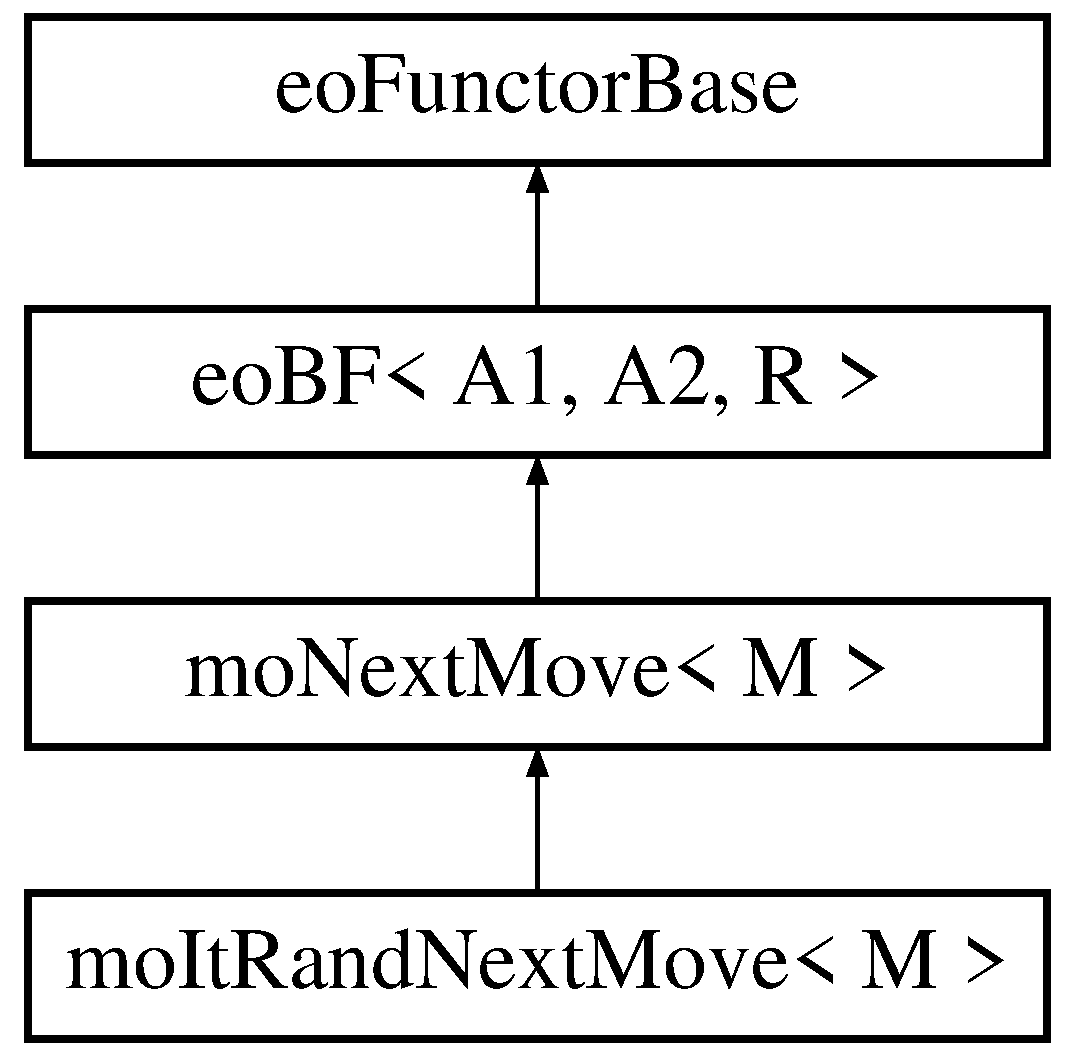
\includegraphics[height=4cm]{classmo_it_rand_next_move}
\end{center}
\end{figure}
\subsection*{Public Member Functions}
\begin{CompactItemize}
\item 
{\bf mo\-It\-Rand\-Next\-Move} ({\bf mo\-Rand\-Move}$<$ M $>$ \&\_\-random\_\-move\_\-generator, unsigned int \_\-iteration\_\-maximum\_\-number)
\begin{CompactList}\small\item\em The constructor. \item\end{CompactList}\item 
bool {\bf operator()} (M \&\_\-move, const {\bf EOT} \&\_\-solution)
\begin{CompactList}\small\item\em Generation of a new move. \item\end{CompactList}\end{CompactItemize}
\subsection*{Private Types}
\begin{CompactItemize}
\item 
typedef M::EOType {\bf EOT}\label{classmo_it_rand_next_move_y0}

\begin{CompactList}\small\item\em Alias for the type. \item\end{CompactList}\end{CompactItemize}
\subsection*{Private Attributes}
\begin{CompactItemize}
\item 
{\bf mo\-Rand\-Move}$<$ M $>$ \& {\bf random\_\-move\_\-generator}\label{classmo_it_rand_next_move_r0}

\begin{CompactList}\small\item\em A move generator (generally randomly). \item\end{CompactList}\item 
unsigned int {\bf iteration\_\-maximum\_\-number}\label{classmo_it_rand_next_move_r1}

\begin{CompactList}\small\item\em Iteration maximum number. \item\end{CompactList}\item 
unsigned int {\bf iteration\_\-number}\label{classmo_it_rand_next_move_r2}

\begin{CompactList}\small\item\em Iteration current number. \item\end{CompactList}\end{CompactItemize}


\subsection{Detailed Description}
\subsubsection*{template$<$class M$>$ class mo\-It\-Rand\-Next\-Move$<$ M $>$}

One of the possible {\bf mo\-Next\-Move}{\rm (p.\,\pageref{classmo_next_move})}. 

This class is a move ({\bf mo\-Move}{\rm (p.\,\pageref{classmo_move})}) generator with a bound for the maximum number of iterations. 



Definition at line 47 of file mo\-It\-Rand\-Next\-Move.h.

\subsection{Constructor \& Destructor Documentation}
\index{moItRandNextMove@{mo\-It\-Rand\-Next\-Move}!moItRandNextMove@{moItRandNextMove}}
\index{moItRandNextMove@{moItRandNextMove}!moItRandNextMove@{mo\-It\-Rand\-Next\-Move}}
\subsubsection{\setlength{\rightskip}{0pt plus 5cm}template$<$class M$>$ {\bf mo\-It\-Rand\-Next\-Move}$<$ M $>$::{\bf mo\-It\-Rand\-Next\-Move} ({\bf mo\-Rand\-Move}$<$ M $>$ \& {\em \_\-random\_\-move\_\-generator}, unsigned int {\em \_\-iteration\_\-maximum\_\-number})\hspace{0.3cm}{\tt  [inline]}}\label{classmo_it_rand_next_move_a0}


The constructor. 

Parameters only for initialising the attributes.

\begin{Desc}
\item[Parameters:]
\begin{description}
\item[{\em \_\-random\_\-move\_\-generator}]The random move generator. \item[{\em \_\-iteration\_\-maximum\_\-number}]The iteration maximum number. \end{description}
\end{Desc}


Definition at line 61 of file mo\-It\-Rand\-Next\-Move.h.

References mo\-It\-Rand\-Next\-Move$<$ M $>$::iteration\_\-maximum\_\-number, mo\-It\-Rand\-Next\-Move$<$ M $>$::iteration\_\-number, and mo\-It\-Rand\-Next\-Move$<$ M $>$::random\_\-move\_\-generator.

\subsection{Member Function Documentation}
\index{moItRandNextMove@{mo\-It\-Rand\-Next\-Move}!operator()@{operator()}}
\index{operator()@{operator()}!moItRandNextMove@{mo\-It\-Rand\-Next\-Move}}
\subsubsection{\setlength{\rightskip}{0pt plus 5cm}template$<$class M$>$ bool {\bf mo\-It\-Rand\-Next\-Move}$<$ M $>$::operator() (M \& {\em \_\-move}, const {\bf EOT} \& {\em \_\-solution})\hspace{0.3cm}{\tt  [inline]}}\label{classmo_it_rand_next_move_a1}


Generation of a new move. 

If the maximum number is not already reached, the current move is forgotten and remplaced by another one.

\begin{Desc}
\item[Parameters:]
\begin{description}
\item[{\em \_\-move}]the current move. \item[{\em \_\-solution}]the current solution. \end{description}
\end{Desc}
\begin{Desc}
\item[Returns:]false if the maximum number of iteration is reached, else true. \end{Desc}


Definition at line 73 of file mo\-It\-Rand\-Next\-Move.h.

References mo\-It\-Rand\-Next\-Move$<$ M $>$::EOT, mo\-It\-Rand\-Next\-Move$<$ M $>$::iteration\_\-number, and mo\-It\-Rand\-Next\-Move$<$ M $>$::random\_\-move\_\-generator.

The documentation for this class was generated from the following file:\begin{CompactItemize}
\item 
mo\-It\-Rand\-Next\-Move.h\end{CompactItemize}

\section{mo\-Linear\-Cooling\-Schedule Class Reference}
\label{classmo_linear_cooling_schedule}\index{moLinearCoolingSchedule@{moLinearCoolingSchedule}}
One of the possible \doxyref{mo\-Cooling\-Schedule}{p.}{classmo_cooling_schedule}.  


{\tt \#include $<$mo\-Linear\-Cooling\-Schedule.h$>$}

Inheritance diagram for mo\-Linear\-Cooling\-Schedule::\begin{figure}[H]
\begin{center}
\leavevmode
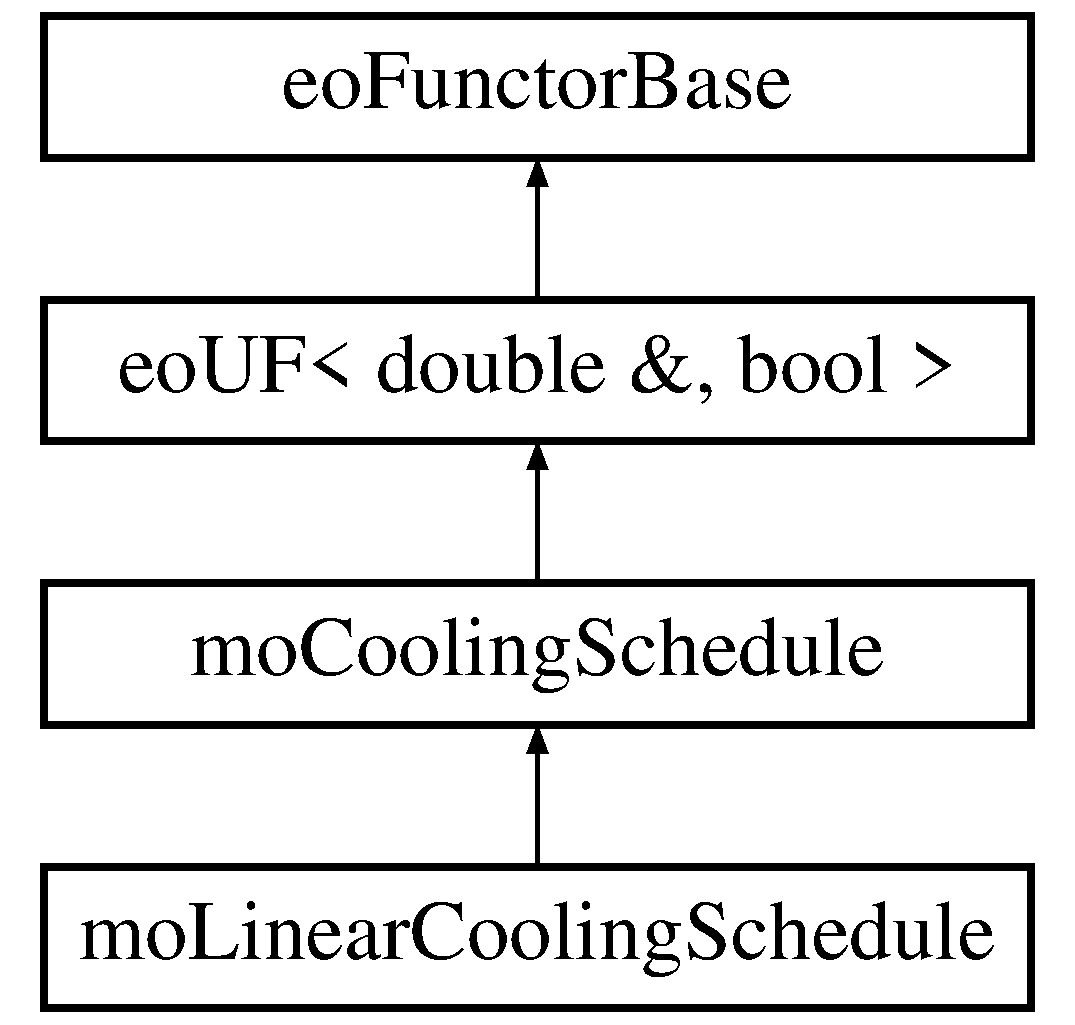
\includegraphics[height=4cm]{classmo_linear_cooling_schedule}
\end{center}
\end{figure}
\subsection*{Public Member Functions}
\begin{CompactItemize}
\item 
\bf{mo\-Linear\-Cooling\-Schedule} (double \_\-threshold, double \_\-quantity)
\begin{CompactList}\small\item\em Simple constructor. \item\end{CompactList}\item 
bool \bf{operator()} (double \&\_\-current\_\-temperature)
\begin{CompactList}\small\item\em \doxyref{Function} which proceeds to the cooling. \item\end{CompactList}\end{CompactItemize}
\subsection*{Private Attributes}
\begin{CompactItemize}
\item 
double \bf{threshold}\label{classmo_linear_cooling_schedule_e7f539f986801ea71392c4a55ba08a76}

\begin{CompactList}\small\item\em The temperature threhold. \item\end{CompactList}\item 
double \bf{quantity}\label{classmo_linear_cooling_schedule_6159dc39ceda89b23ffdab3d6ce8d8ed}

\begin{CompactList}\small\item\em The quantity that allows the temperature to decrease. \item\end{CompactList}\end{CompactItemize}


\subsection{Detailed Description}
One of the possible \doxyref{mo\-Cooling\-Schedule}{p.}{classmo_cooling_schedule}. 

An another very simple cooling schedule, the temperature decrease according to a quantity while the temperature is greater than a threshold. 



Definition at line 46 of file mo\-Linear\-Cooling\-Schedule.h.

\subsection{Constructor \& Destructor Documentation}
\index{moLinearCoolingSchedule@{mo\-Linear\-Cooling\-Schedule}!moLinearCoolingSchedule@{moLinearCoolingSchedule}}
\index{moLinearCoolingSchedule@{moLinearCoolingSchedule}!moLinearCoolingSchedule@{mo\-Linear\-Cooling\-Schedule}}
\subsubsection{\setlength{\rightskip}{0pt plus 5cm}mo\-Linear\-Cooling\-Schedule::mo\-Linear\-Cooling\-Schedule (double {\em \_\-threshold}, double {\em \_\-quantity})\hspace{0.3cm}{\tt  [inline]}}\label{classmo_linear_cooling_schedule_420939ebf57f01d242cbe4eb668dffde}


Simple constructor. 

\begin{Desc}
\item[Parameters:]
\begin{description}
\item[{\em \_\-threshold}]the threshold. \item[{\em \_\-quantity}]the quantity used to descrease the temperature. \end{description}
\end{Desc}


Definition at line 55 of file mo\-Linear\-Cooling\-Schedule.h.

\subsection{Member Function Documentation}
\index{moLinearCoolingSchedule@{mo\-Linear\-Cooling\-Schedule}!operator()@{operator()}}
\index{operator()@{operator()}!moLinearCoolingSchedule@{mo\-Linear\-Cooling\-Schedule}}
\subsubsection{\setlength{\rightskip}{0pt plus 5cm}bool mo\-Linear\-Cooling\-Schedule::operator() (double \& {\em \_\-current\_\-temperature})\hspace{0.3cm}{\tt  [inline, virtual]}}\label{classmo_linear_cooling_schedule_b0a1886aaa7ee2a0c8e929e55ca321ce}


\doxyref{Function} which proceeds to the cooling. 

It decreases the temperature and indicates if it is greater than the threshold.

\begin{Desc}
\item[Parameters:]
\begin{description}
\item[{\em \_\-current\_\-temperature}]The current temperature. \end{description}
\end{Desc}
\begin{Desc}
\item[Returns:]true if the new temperature (current temperature - quantity) is greater than the threshold, false otherwise. \end{Desc}


Implements \bf{eo\-UF$<$ double \&, bool $>$}.

Definition at line 65 of file mo\-Linear\-Cooling\-Schedule.h.

References quantity, and threshold.

The documentation for this class was generated from the following file:\begin{CompactItemize}
\item 
mo\-Linear\-Cooling\-Schedule.h\end{CompactItemize}

\section{mo\-LSCheck\-Point$<$ M $>$ Class Template Reference}
\label{classmo_l_s_check_point}\index{moLSCheckPoint@{moLSCheckPoint}}
Class which allows a checkpointing system.  


{\tt \#include $<$mo\-LSCheck\-Point.h$>$}

\subsection*{Public Member Functions}
\begin{CompactItemize}
\item 
void \bf{operator()} (const M \&\_\-move, const typename M::EOType \&\_\-solution)
\begin{CompactList}\small\item\em Function which launches the checkpointing. \item\end{CompactList}\item 
void \bf{add} (eo\-BF$<$ const M \&, const typename M::EOType \&, void $>$ \&\_\-function)
\begin{CompactList}\small\item\em Procedure which add a new function to the function vector. \item\end{CompactList}\end{CompactItemize}
\subsection*{Private Attributes}
\begin{CompactItemize}
\item 
std::vector$<$ eo\-BF$<$ const M \&, const typename M::EOType \&, void $>$ $\ast$ $>$ \bf{functions}\label{classmo_l_s_check_point_56a7427a6aebac7955c22bab302c050a}

\begin{CompactList}\small\item\em Vector of functions. \item\end{CompactList}\end{CompactItemize}


\subsection{Detailed Description}
\subsubsection*{template$<$class M$>$ class mo\-LSCheck\-Point$<$ M $>$}

Class which allows a checkpointing system. 

Thanks to this class, at each iteration, additionnal function can be used (and not only one). 



Definition at line 46 of file mo\-LSCheck\-Point.h.

\subsection{Member Function Documentation}
\index{moLSCheckPoint@{mo\-LSCheck\-Point}!operator()@{operator()}}
\index{operator()@{operator()}!moLSCheckPoint@{mo\-LSCheck\-Point}}
\subsubsection{\setlength{\rightskip}{0pt plus 5cm}template$<$class M$>$ void \bf{mo\-LSCheck\-Point}$<$ M $>$::operator() (const M \& {\em \_\-move}, const typename M::EOType \& {\em \_\-solution})\hspace{0.3cm}{\tt  [inline]}}\label{classmo_l_s_check_point_e9b9d41e40dd7bab648327686b2b938d}


Function which launches the checkpointing. 

Each saved function is used on the current move and the current solution.

\begin{Desc}
\item[Parameters:]
\begin{description}
\item[{\em \_\-move}]a move. \item[{\em \_\-solution}]a solution. \end{description}
\end{Desc}


Definition at line 57 of file mo\-LSCheck\-Point.h.

References mo\-LSCheck\-Point$<$ M $>$::functions.\index{moLSCheckPoint@{mo\-LSCheck\-Point}!add@{add}}
\index{add@{add}!moLSCheckPoint@{mo\-LSCheck\-Point}}
\subsubsection{\setlength{\rightskip}{0pt plus 5cm}template$<$class M$>$ void \bf{mo\-LSCheck\-Point}$<$ M $>$::add (eo\-BF$<$ const M \&, const typename M::EOType \&, void $>$ \& {\em \_\-function})\hspace{0.3cm}{\tt  [inline]}}\label{classmo_l_s_check_point_f95f2dc556cdfbdc81688562ca95202d}


Procedure which add a new function to the function vector. 

The new function is added at the end of the vector. \begin{Desc}
\item[Parameters:]
\begin{description}
\item[{\em \_\-function}]a new function to add. \end{description}
\end{Desc}


Definition at line 72 of file mo\-LSCheck\-Point.h.

References mo\-LSCheck\-Point$<$ M $>$::functions.

The documentation for this class was generated from the following file:\begin{CompactItemize}
\item 
mo\-LSCheck\-Point.h\end{CompactItemize}

\section{moMove$<$ EOT $>$ Class Template Reference}
\label{classmo_move}\index{moMove@{moMove}}
Definition of a move.  


{\tt \#include $<$moMove.h$>$}

Inheritance diagram for moMove$<$ EOT $>$::\begin{figure}[H]
\begin{center}
\leavevmode
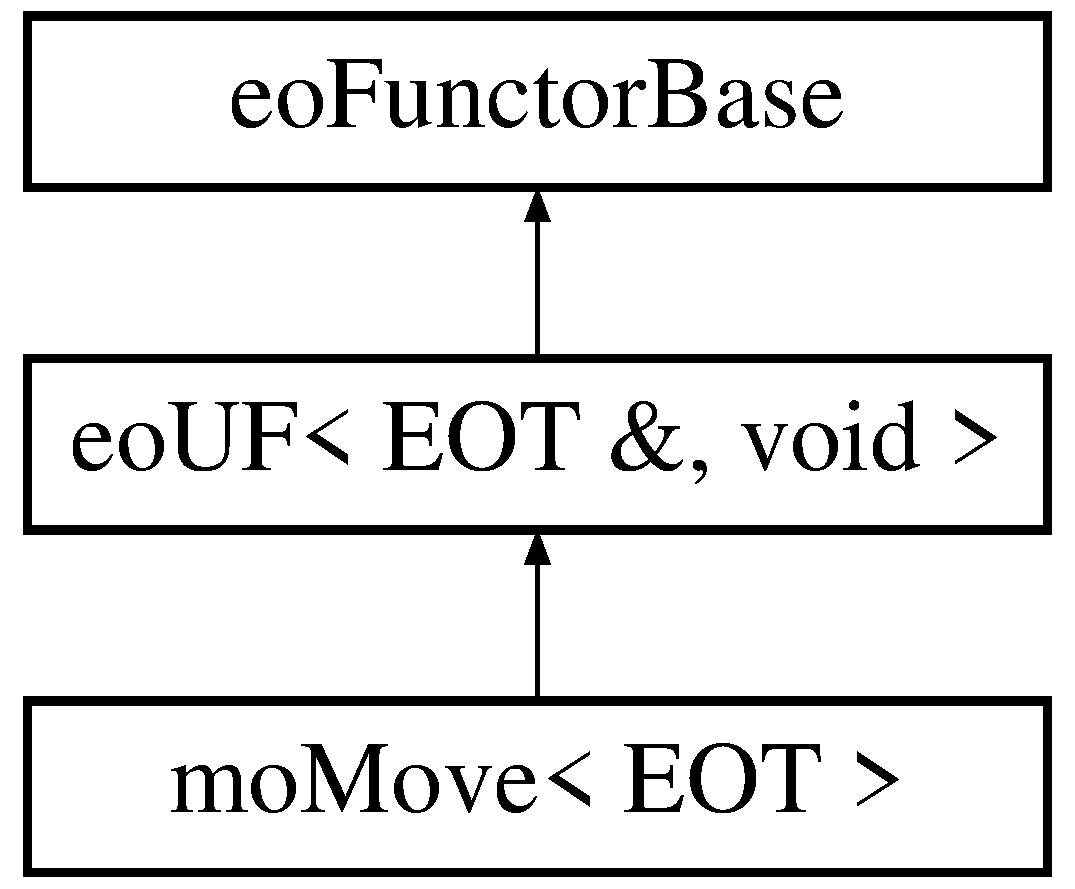
\includegraphics[height=3cm]{classmo_move}
\end{center}
\end{figure}
\subsection*{Public Types}
\begin{CompactItemize}
\item 
typedef EOT {\bf EOType}\label{classmo_move_7fb853a91ba1319530529e515380bbba}

\begin{CompactList}\small\item\em Alias for the type. \item\end{CompactList}\end{CompactItemize}


\subsection{Detailed Description}
\subsubsection*{template$<$class EOT$>$ class moMove$<$ EOT $>$}

Definition of a move. 

A move transforms a solution to another close solution. It describes how a solution can be modified to another one. 

Definition at line 49 of file moMove.h.

The documentation for this class was generated from the following file:\begin{CompactItemize}
\item 
moMove.h\end{CompactItemize}

\section{mo\-Move\-Expl$<$ M $>$ Class Template Reference}
\label{classmo_move_expl}\index{moMoveExpl@{moMoveExpl}}
Description of a move ({\bf mo\-Move}{\rm (p.\,\pageref{classmo_move})}) explorer.  


{\tt \#include $<$mo\-Move\-Expl.h$>$}

Inheritance diagram for mo\-Move\-Expl$<$ M $>$::\begin{figure}[H]
\begin{center}
\leavevmode
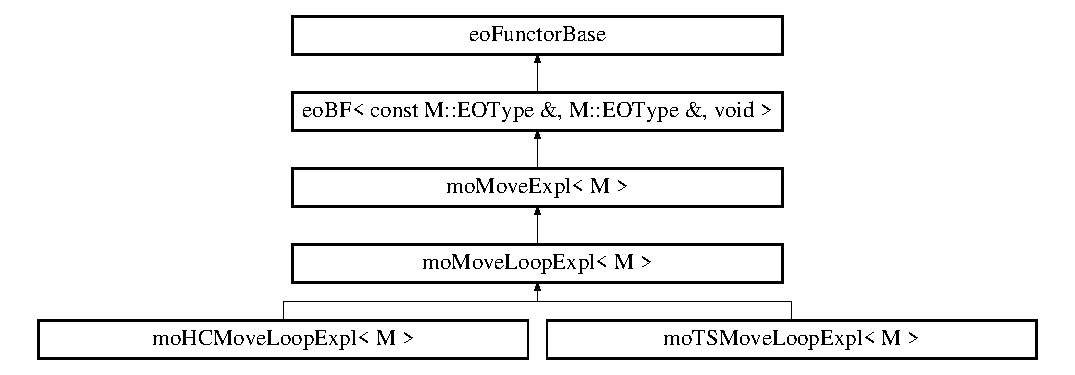
\includegraphics[height=4.59016cm]{classmo_move_expl}
\end{center}
\end{figure}


\subsection{Detailed Description}
\subsubsection*{template$<$class M$>$ class mo\-Move\-Expl$<$ M $>$}

Description of a move ({\bf mo\-Move}{\rm (p.\,\pageref{classmo_move})}) explorer. 

Only a description...See {\bf mo\-Move\-Loop\-Expl}{\rm (p.\,\pageref{classmo_move_loop_expl})}. 



Definition at line 46 of file mo\-Move\-Expl.h.

The documentation for this class was generated from the following file:\begin{CompactItemize}
\item 
mo\-Move\-Expl.h\end{CompactItemize}

\section{mo\-Move\-Incr\-Eval$<$ M $>$ Class Template Reference}
\label{classmo_move_incr_eval}\index{moMoveIncrEval@{moMoveIncrEval}}
(generally) Efficient evaluation function based a move and a solution.  


{\tt \#include $<$mo\-Move\-Incr\-Eval.h$>$}

Inheritance diagram for mo\-Move\-Incr\-Eval$<$ M $>$::\begin{figure}[H]
\begin{center}
\leavevmode
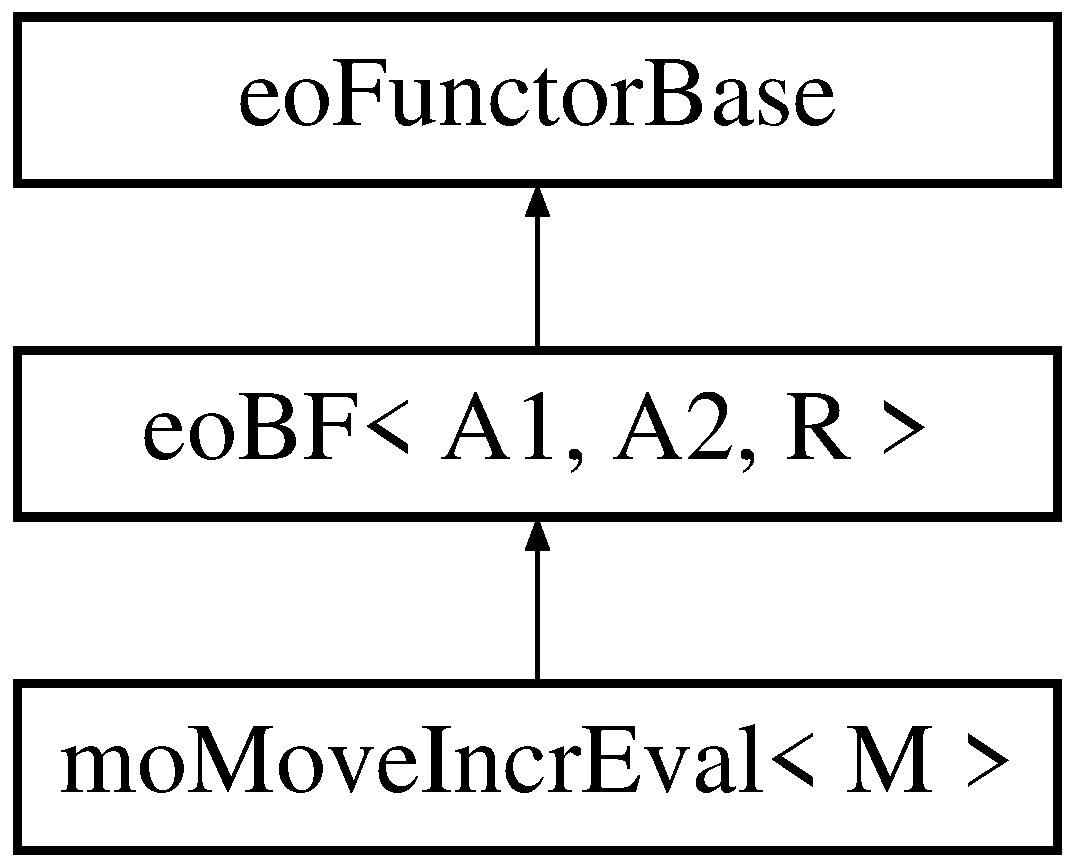
\includegraphics[height=3cm]{classmo_move_incr_eval}
\end{center}
\end{figure}


\subsection{Detailed Description}
\subsubsection*{template$<$class M$>$ class mo\-Move\-Incr\-Eval$<$ M $>$}

(generally) Efficient evaluation function based a move and a solution. 

From a move and a solution, it computes a new fitness that could be associated to the solution if this one is updated. 



Definition at line 49 of file mo\-Move\-Incr\-Eval.h.

The documentation for this class was generated from the following file:\begin{CompactItemize}
\item 
mo\-Move\-Incr\-Eval.h\end{CompactItemize}

\section{mo\-Move\-Init$<$ M $>$ Class Template Reference}
\label{classmo_move_init}\index{moMoveInit@{moMoveInit}}
Move (\doxyref{mo\-Move}{p.}{classmo_move}) initializer.  


{\tt \#include $<$mo\-Move\-Init.h$>$}



\subsection{Detailed Description}
\subsubsection*{template$<$class M$>$ class mo\-Move\-Init$<$ M $>$}

Move (\doxyref{mo\-Move}{p.}{classmo_move}) initializer. 

Class which allows to initiase a move. Only a description... An object that herits from this class needs to be designed to be used. 



Definition at line 47 of file mo\-Move\-Init.h.

The documentation for this class was generated from the following file:\begin{CompactItemize}
\item 
mo\-Move\-Init.h\end{CompactItemize}

\section{mo\-Move\-Loop\-Expl$<$ M $>$ Class Template Reference}
\label{classmo_move_loop_expl}\index{moMoveLoopExpl@{moMoveLoopExpl}}
Class which describes an iterative explorer.  


{\tt \#include $<$mo\-Move\-Loop\-Expl.h$>$}

Inheritance diagram for mo\-Move\-Loop\-Expl$<$ M $>$::\begin{figure}[H]
\begin{center}
\leavevmode
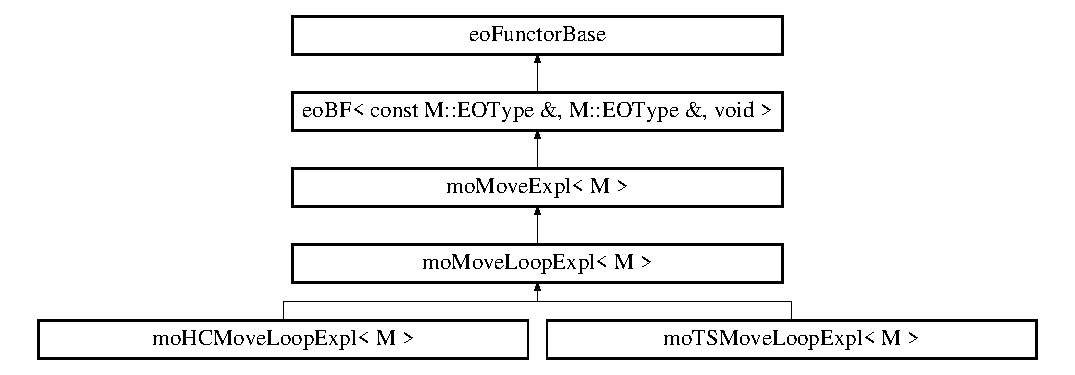
\includegraphics[height=3cm]{classmo_move_loop_expl}
\end{center}
\end{figure}


\subsection{Detailed Description}
\subsubsection*{template$<$class M$>$ class mo\-Move\-Loop\-Expl$<$ M $>$}

Class which describes an iterative explorer. 

Only a description... \doxyref{mo\-HCMove\-Loop\-Expl}{p.}{classmo_h_c_move_loop_expl} and \doxyref{mo\-TSMove\-Loop\-Expl}{p.}{classmo_t_s_move_loop_expl} are exemples of class that are a \doxyref{mo\-Move\-Loop\-Expl}{p.}{classmo_move_loop_expl}. 



Definition at line 47 of file mo\-Move\-Loop\-Expl.h.

The documentation for this class was generated from the following file:\begin{CompactItemize}
\item 
mo\-Move\-Loop\-Expl.h\end{CompactItemize}

\section{moMoveSelect$<$ M $>$ Class Template Reference}
\label{classmo_move_select}\index{moMoveSelect@{moMoveSelect}}
Class that describes a move selector (\doxyref{moMove}{p.}{classmo_move}).  


{\tt \#include $<$moMoveSelect.h$>$}

Inheritance diagram for moMoveSelect$<$ M $>$::\begin{figure}[H]
\begin{center}
\leavevmode
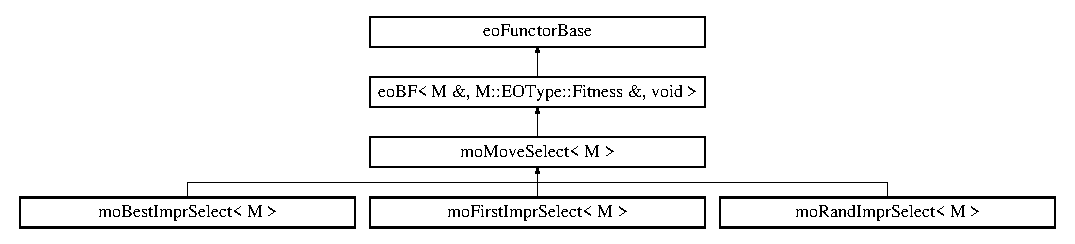
\includegraphics[height=2.82828cm]{classmo_move_select}
\end{center}
\end{figure}
\subsection*{Public Types}
\begin{CompactItemize}
\item 
typedef M::EOType::Fitness {\bf Fitness}\label{classmo_move_select_8148ccc0e6fbd209c3fe6829559895c8}

\begin{CompactList}\small\item\em Alias for the fitness. \item\end{CompactList}\end{CompactItemize}
\subsection*{Public Member Functions}
\begin{CompactItemize}
\item 
virtual void {\bf init} (const {\bf Fitness} \&\_\-fitness)=0
\begin{CompactList}\small\item\em Procedure which initialises all that the move selector needs including the initial fitness. \item\end{CompactList}\item 
virtual bool {\bf update} (const M \&\_\-move, const {\bf Fitness} \&\_\-fitness)=0
\begin{CompactList}\small\item\em {\bf Function} which updates the best solutions. \item\end{CompactList}\end{CompactItemize}


\subsection{Detailed Description}
\subsubsection*{template$<$class M$>$ class moMoveSelect$<$ M $>$}

Class that describes a move selector (\doxyref{moMove}{p.}{classmo_move}). 

It iteratively considers some moves (\doxyref{moMove}{p.}{classmo_move}) and their associated fitnesses. The best move is so regularly updated. At any time, it could be accessed. 

Definition at line 50 of file moMoveSelect.h.

\subsection{Member Function Documentation}
\index{moMoveSelect@{moMoveSelect}!init@{init}}
\index{init@{init}!moMoveSelect@{moMoveSelect}}
\subsubsection{\setlength{\rightskip}{0pt plus 5cm}template$<$class M$>$ virtual void {\bf moMoveSelect}$<$ M $>$::init (const {\bf Fitness} \& {\em \_\-fitness})\hspace{0.3cm}{\tt  [pure virtual]}}\label{classmo_move_select_58038bd859632c1bd022d23d9792bdca}


Procedure which initialises all that the move selector needs including the initial fitness. 

In order to know the fitness of the solution, for which the neighborhood will be soon explored

\begin{Desc}
\item[Parameters:]
\begin{description}
\item[{\em \_\-fitness}]the current fitness. \end{description}
\end{Desc}


Implemented in {\bf moBestImprSelect$<$ M $>$} \doxyref{}{p.}{classmo_best_impr_select_83f961549986b8ad94692e433aa79114}, {\bf moFirstImprSelect$<$ M $>$} \doxyref{}{p.}{classmo_first_impr_select_a923437ecc3db50e7052b002a9a1bbf8}, and {\bf moRandImprSelect$<$ M $>$} \doxyref{}{p.}{classmo_rand_impr_select_7af99966b31aa387ecef74fd307a42e8}.\index{moMoveSelect@{moMoveSelect}!update@{update}}
\index{update@{update}!moMoveSelect@{moMoveSelect}}
\subsubsection{\setlength{\rightskip}{0pt plus 5cm}template$<$class M$>$ virtual bool {\bf moMoveSelect}$<$ M $>$::update (const M \& {\em \_\-move}, const {\bf Fitness} \& {\em \_\-fitness})\hspace{0.3cm}{\tt  [pure virtual]}}\label{classmo_move_select_5b4d3b2f030cca80c563c3db0c4af404}


{\bf Function} which updates the best solutions. 

\begin{Desc}
\item[Parameters:]
\begin{description}
\item[{\em \_\-move}]a new move. \item[{\em \_\-fitness}]a fitness linked to the new move. \end{description}
\end{Desc}
\begin{Desc}
\item[Returns:]a boolean that expresses the need to resume the exploration. \end{Desc}


Implemented in {\bf moBestImprSelect$<$ M $>$} \doxyref{}{p.}{classmo_best_impr_select_5c0729fd316b0ef78406bce5ca91de2a}, {\bf moFirstImprSelect$<$ M $>$} \doxyref{}{p.}{classmo_first_impr_select_f68b7ee7b35bf7347c16006f0587d313}, and {\bf moRandImprSelect$<$ M $>$} \doxyref{}{p.}{classmo_rand_impr_select_b20cfd0164266aa75960cba3c1673f69}.

The documentation for this class was generated from the following file:\begin{CompactItemize}
\item 
moMoveSelect.h\end{CompactItemize}

\section{mo\-Next\-Move$<$ M $>$ Class Template Reference}
\label{classmo_next_move}\index{moNextMove@{moNextMove}}
Class which allows to generate a new move (\doxyref{mo\-Move}{p.}{classmo_move}).  


{\tt \#include $<$mo\-Next\-Move.h$>$}

Inheritance diagram for mo\-Next\-Move$<$ M $>$::\begin{figure}[H]
\begin{center}
\leavevmode
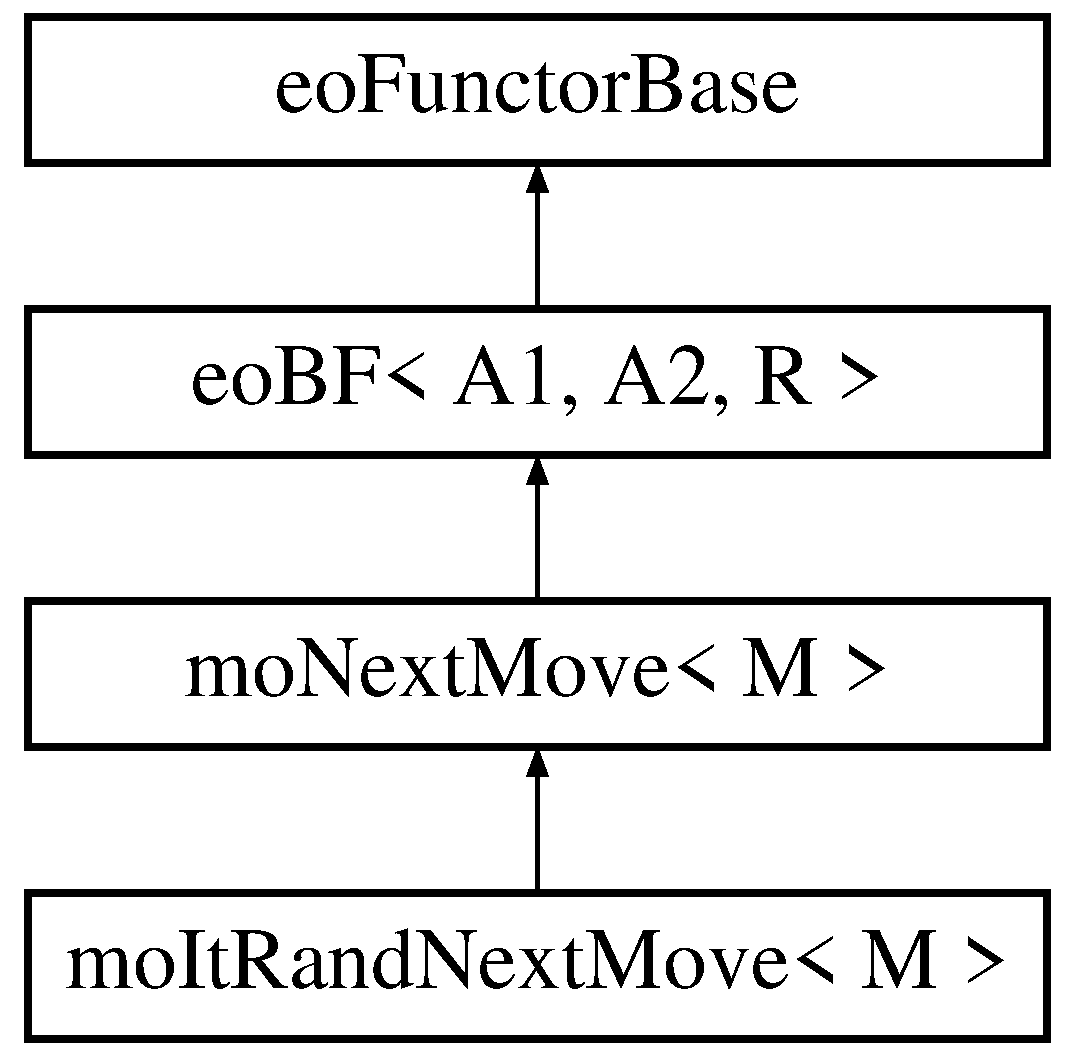
\includegraphics[height=4cm]{classmo_next_move}
\end{center}
\end{figure}


\subsection{Detailed Description}
\subsubsection*{template$<$class M$>$ class mo\-Next\-Move$<$ M $>$}

Class which allows to generate a new move (\doxyref{mo\-Move}{p.}{classmo_move}). 

Useful for the explorer (for \doxyref{mo\-TS}{p.}{classmo_t_s} or \doxyref{mo\-HC}{p.}{classmo_h_c}). Does nothing... An object that herits from this class needs to be designed for being used. 



Definition at line 47 of file mo\-Next\-Move.h.

The documentation for this class was generated from the following file:\begin{CompactItemize}
\item 
mo\-Next\-Move.h\end{CompactItemize}

\section{mo\-No\-Aspir\-Crit$<$ M $>$ Class Template Reference}
\label{classmo_no_aspir_crit}\index{moNoAspirCrit@{moNoAspirCrit}}
One of the possible aspiration criterion ({\bf mo\-Aspir\-Crit}{\rm (p.\,\pageref{classmo_aspir_crit})}).  


{\tt \#include $<$mo\-No\-Aspir\-Crit.h$>$}

Inheritance diagram for mo\-No\-Aspir\-Crit$<$ M $>$::\begin{figure}[H]
\begin{center}
\leavevmode
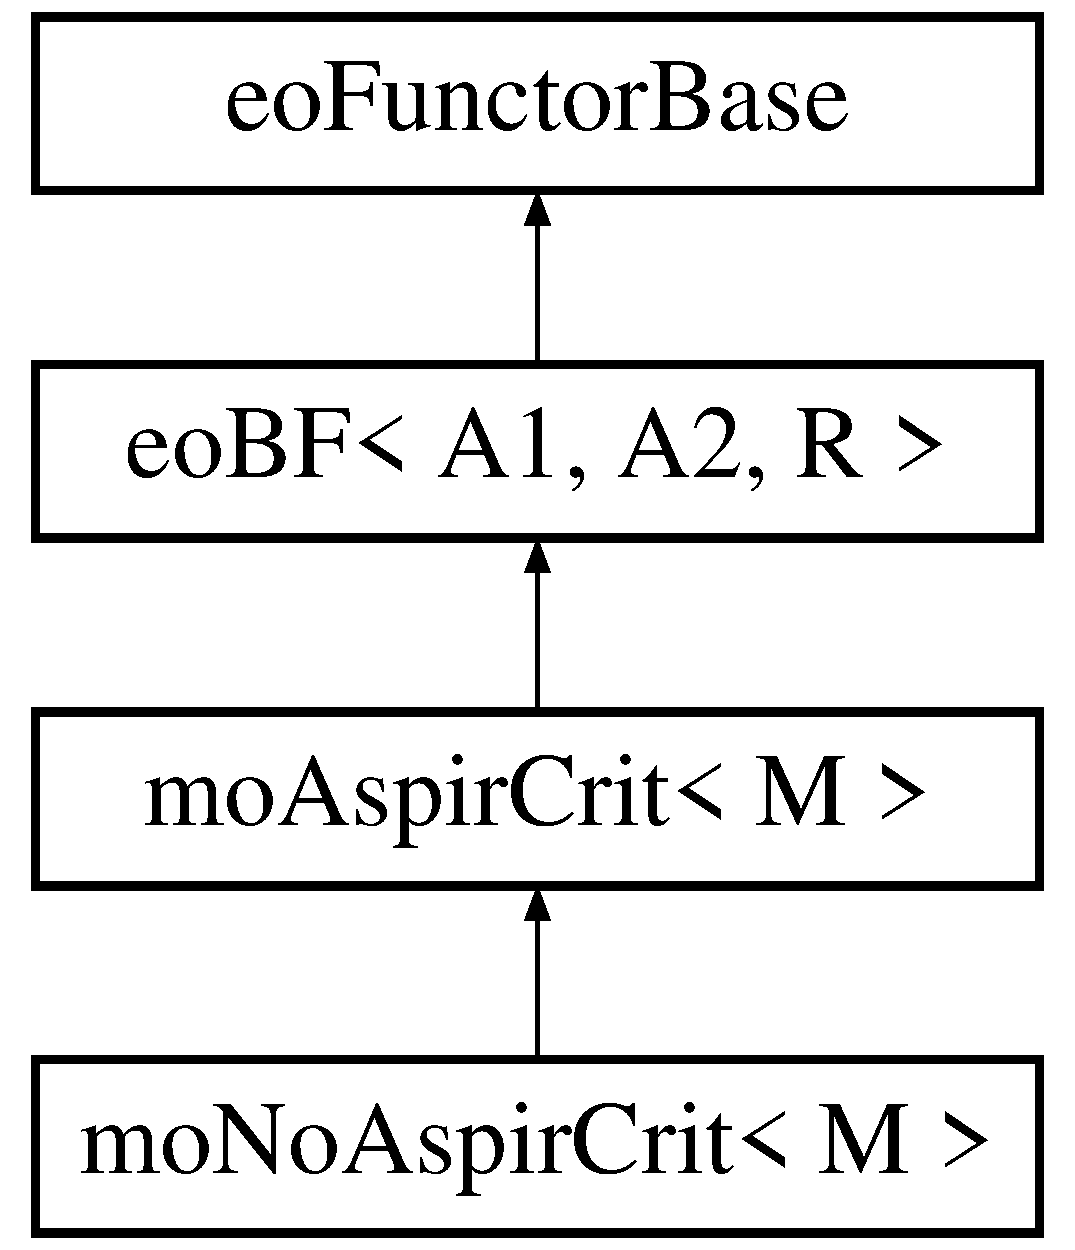
\includegraphics[height=4cm]{classmo_no_aspir_crit}
\end{center}
\end{figure}
\subsection*{Public Member Functions}
\begin{CompactItemize}
\item 
bool {\bf operator()} (const M \&\_\-move, const typename M::EOType::Fitness \&\_\-fitness)
\begin{CompactList}\small\item\em Function which describes the aspiration criterion behaviour. \item\end{CompactList}\item 
void {\bf init} ()
\begin{CompactList}\small\item\em Procedure which initialises all that needs a mo\-No\-Aspir\-Crit. \item\end{CompactList}\end{CompactItemize}


\subsection{Detailed Description}
\subsubsection*{template$<$class M$>$ class mo\-No\-Aspir\-Crit$<$ M $>$}

One of the possible aspiration criterion ({\bf mo\-Aspir\-Crit}{\rm (p.\,\pageref{classmo_aspir_crit})}). 

The simplest : never satisfied. 



Definition at line 47 of file mo\-No\-Aspir\-Crit.h.

\subsection{Member Function Documentation}
\index{moNoAspirCrit@{mo\-No\-Aspir\-Crit}!operator()@{operator()}}
\index{operator()@{operator()}!moNoAspirCrit@{mo\-No\-Aspir\-Crit}}
\subsubsection{\setlength{\rightskip}{0pt plus 5cm}template$<$class M$>$ bool {\bf mo\-No\-Aspir\-Crit}$<$ M $>$::operator() (const M \& {\em \_\-move}, const typename M::EOType::Fitness \& {\em \_\-fitness})\hspace{0.3cm}{\tt  [inline]}}\label{classmo_no_aspir_crit_a0}


Function which describes the aspiration criterion behaviour. 

Does nothing.

\begin{Desc}
\item[Parameters:]
\begin{description}
\item[{\em \_\-move}]a move. \item[{\em \_\-fitness}]a fitness. \end{description}
\end{Desc}
\begin{Desc}
\item[Returns:]false. \end{Desc}


Definition at line 59 of file mo\-No\-Aspir\-Crit.h.\index{moNoAspirCrit@{mo\-No\-Aspir\-Crit}!init@{init}}
\index{init@{init}!moNoAspirCrit@{mo\-No\-Aspir\-Crit}}
\subsubsection{\setlength{\rightskip}{0pt plus 5cm}template$<$class M$>$ void {\bf mo\-No\-Aspir\-Crit}$<$ M $>$::init ()\hspace{0.3cm}{\tt  [inline, virtual]}}\label{classmo_no_aspir_crit_a1}


Procedure which initialises all that needs a mo\-No\-Aspir\-Crit. 

Nothing... 

Implements {\bf mo\-Aspir\-Crit$<$ M $>$} {\rm (p.\,\pageref{classmo_aspir_crit_a0})}.

Definition at line 73 of file mo\-No\-Aspir\-Crit.h.

The documentation for this class was generated from the following file:\begin{CompactItemize}
\item 
mo\-No\-Aspir\-Crit.h\end{CompactItemize}

\section{mo\-No\-Fit\-Impr\-Sol\-Continue$<$ EOT $>$ Class Template Reference}
\label{classmo_no_fit_impr_sol_continue}\index{moNoFitImprSolContinue@{moNoFitImprSolContinue}}
One possible stop criterion for a solution-based heuristic.  


{\tt \#include $<$mo\-No\-Fit\-Impr\-Sol\-Continue.h$>$}

Inheritance diagram for mo\-No\-Fit\-Impr\-Sol\-Continue$<$ EOT $>$::\begin{figure}[H]
\begin{center}
\leavevmode
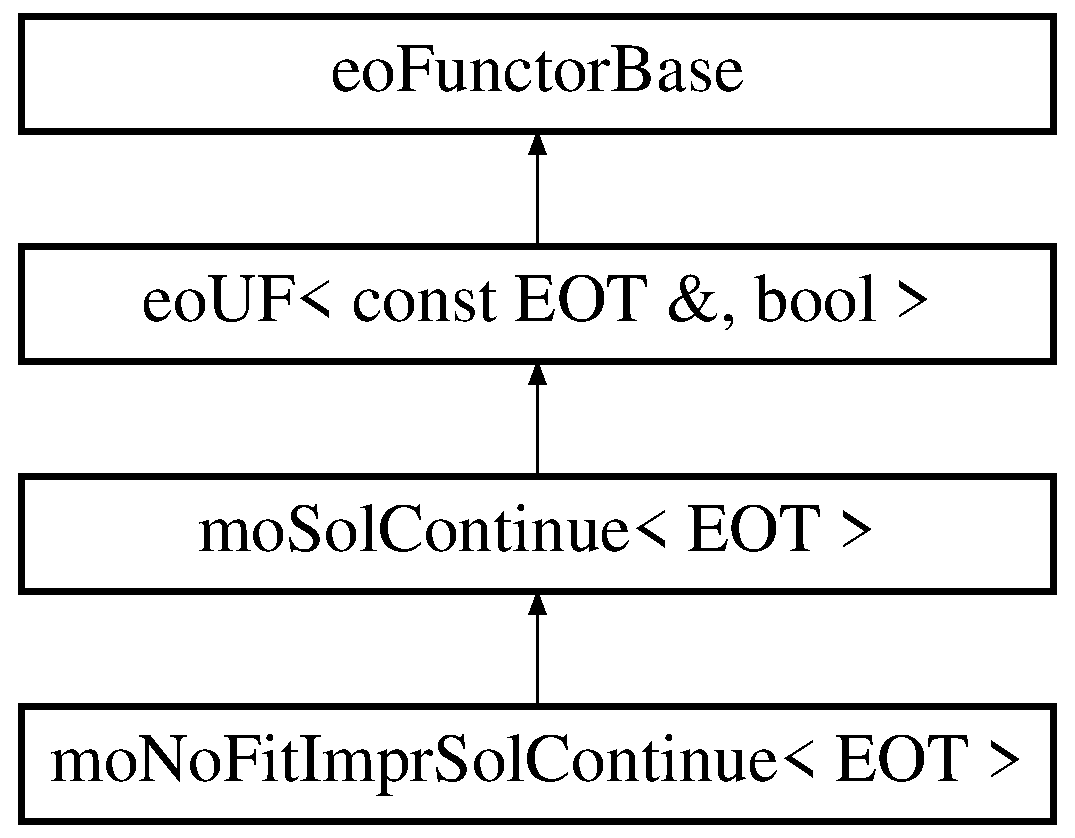
\includegraphics[height=4cm]{classmo_no_fit_impr_sol_continue}
\end{center}
\end{figure}
\subsection*{Public Types}
\begin{CompactItemize}
\item 
typedef EOT::Fitness {\bf Fitness}\label{classmo_no_fit_impr_sol_continue_w0}

\begin{CompactList}\small\item\em Alias for the fitness. \item\end{CompactList}\end{CompactItemize}
\subsection*{Public Member Functions}
\begin{CompactItemize}
\item 
{\bf mo\-No\-Fit\-Impr\-Sol\-Continue} (unsigned int \_\-max\-Number\-Of\-Iteration\-Without\-Improvement)
\begin{CompactList}\small\item\em Basic constructor. \item\end{CompactList}\item 
bool {\bf operator()} (const EOT \&\_\-solution)
\begin{CompactList}\small\item\em Function that activates the stopping criterion. \item\end{CompactList}\item 
void {\bf init} ()
\begin{CompactList}\small\item\em Procedure which allows to initialise all the stuff needed. \item\end{CompactList}\end{CompactItemize}
\subsection*{Private Attributes}
\begin{CompactItemize}
\item 
unsigned int {\bf max\-Number\-Of\-Iterations\-Without\-Improvement}\label{classmo_no_fit_impr_sol_continue_r0}

\begin{CompactList}\small\item\em Maximum number of iterations without improvement allowed. \item\end{CompactList}\item 
bool {\bf first\-Fitness\-Saved}\label{classmo_no_fit_impr_sol_continue_r1}

\begin{CompactList}\small\item\em Flag that this is the first time that the fitness is used. \item\end{CompactList}\item 
{\bf Fitness} {\bf fitness}\label{classmo_no_fit_impr_sol_continue_r2}

\begin{CompactList}\small\item\em Current Fitness. \item\end{CompactList}\item 
unsigned int {\bf counter}\label{classmo_no_fit_impr_sol_continue_r3}

\begin{CompactList}\small\item\em The iteration couter. \item\end{CompactList}\end{CompactItemize}


\subsection{Detailed Description}
\subsubsection*{template$<$class EOT$>$ class mo\-No\-Fit\-Impr\-Sol\-Continue$<$ EOT $>$}

One possible stop criterion for a solution-based heuristic. 

The stop criterion corresponds to a maximum number of iterations without improvement. 



Definition at line 46 of file mo\-No\-Fit\-Impr\-Sol\-Continue.h.

\subsection{Constructor \& Destructor Documentation}
\index{moNoFitImprSolContinue@{mo\-No\-Fit\-Impr\-Sol\-Continue}!moNoFitImprSolContinue@{moNoFitImprSolContinue}}
\index{moNoFitImprSolContinue@{moNoFitImprSolContinue}!moNoFitImprSolContinue@{mo\-No\-Fit\-Impr\-Sol\-Continue}}
\subsubsection{\setlength{\rightskip}{0pt plus 5cm}template$<$class EOT$>$ {\bf mo\-No\-Fit\-Impr\-Sol\-Continue}$<$ EOT $>$::{\bf mo\-No\-Fit\-Impr\-Sol\-Continue} (unsigned int {\em \_\-max\-Number\-Of\-Iteration\-Without\-Improvement})\hspace{0.3cm}{\tt  [inline]}}\label{classmo_no_fit_impr_sol_continue_a0}


Basic constructor. 

\begin{Desc}
\item[Parameters:]
\begin{description}
\item[{\em \_\-max\-Number\-Of\-Iteration\-Without\-Improvement}]The number of iterations without fitness improvement to reach for stop. \end{description}
\end{Desc}


Definition at line 57 of file mo\-No\-Fit\-Impr\-Sol\-Continue.h.

References mo\-No\-Fit\-Impr\-Sol\-Continue$<$ EOT $>$::counter, mo\-No\-Fit\-Impr\-Sol\-Continue$<$ EOT $>$::first\-Fitness\-Saved, and mo\-No\-Fit\-Impr\-Sol\-Continue$<$ EOT $>$::max\-Number\-Of\-Iterations\-Without\-Improvement.

\subsection{Member Function Documentation}
\index{moNoFitImprSolContinue@{mo\-No\-Fit\-Impr\-Sol\-Continue}!operator()@{operator()}}
\index{operator()@{operator()}!moNoFitImprSolContinue@{mo\-No\-Fit\-Impr\-Sol\-Continue}}
\subsubsection{\setlength{\rightskip}{0pt plus 5cm}template$<$class EOT$>$ bool {\bf mo\-No\-Fit\-Impr\-Sol\-Continue}$<$ EOT $>$::operator() (const EOT \& {\em \_\-solution})\hspace{0.3cm}{\tt  [inline, virtual]}}\label{classmo_no_fit_impr_sol_continue_a1}


Function that activates the stopping criterion. 

Indicates if the fitness has not been improved since a given number of iterations (after a minimum of iterations). \begin{Desc}
\item[Parameters:]
\begin{description}
\item[{\em \_\-solution}]the current solution. \end{description}
\end{Desc}
\begin{Desc}
\item[Returns:]true or false. \end{Desc}


Implements {\bf eo\-UF$<$ const EOT \&, bool $>$}.

Definition at line 67 of file mo\-No\-Fit\-Impr\-Sol\-Continue.h.

References mo\-No\-Fit\-Impr\-Sol\-Continue$<$ EOT $>$::counter, mo\-No\-Fit\-Impr\-Sol\-Continue$<$ EOT $>$::first\-Fitness\-Saved, and mo\-No\-Fit\-Impr\-Sol\-Continue$<$ EOT $>$::fitness.\index{moNoFitImprSolContinue@{mo\-No\-Fit\-Impr\-Sol\-Continue}!init@{init}}
\index{init@{init}!moNoFitImprSolContinue@{mo\-No\-Fit\-Impr\-Sol\-Continue}}
\subsubsection{\setlength{\rightskip}{0pt plus 5cm}template$<$class EOT$>$ void {\bf mo\-No\-Fit\-Impr\-Sol\-Continue}$<$ EOT $>$::init ()\hspace{0.3cm}{\tt  [inline, virtual]}}\label{classmo_no_fit_impr_sol_continue_a2}


Procedure which allows to initialise all the stuff needed. 

It can be also used to reinitialize all the needed things. 

Implements {\bf mo\-Sol\-Continue$<$ EOT $>$} {\rm (p.\,\pageref{classmo_sol_continue_a0})}.

Definition at line 102 of file mo\-No\-Fit\-Impr\-Sol\-Continue.h.

References mo\-No\-Fit\-Impr\-Sol\-Continue$<$ EOT $>$::counter, and mo\-No\-Fit\-Impr\-Sol\-Continue$<$ EOT $>$::first\-Fitness\-Saved.

The documentation for this class was generated from the following file:\begin{CompactItemize}
\item 
mo\-No\-Fit\-Impr\-Sol\-Continue.h\end{CompactItemize}

\section{mo\-Rand\-Impr\-Select$<$ M $>$ Class Template Reference}
\label{classmo_rand_impr_select}\index{moRandImprSelect@{moRandImprSelect}}
One of the possible \doxyref{mo\-Move}{p.}{classmo_move} selector (\doxyref{mo\-Move\-Select}{p.}{classmo_move_select}).  


{\tt \#include $<$mo\-Rand\-Impr\-Select.h$>$}

Inheritance diagram for mo\-Rand\-Impr\-Select$<$ M $>$::\begin{figure}[H]
\begin{center}
\leavevmode
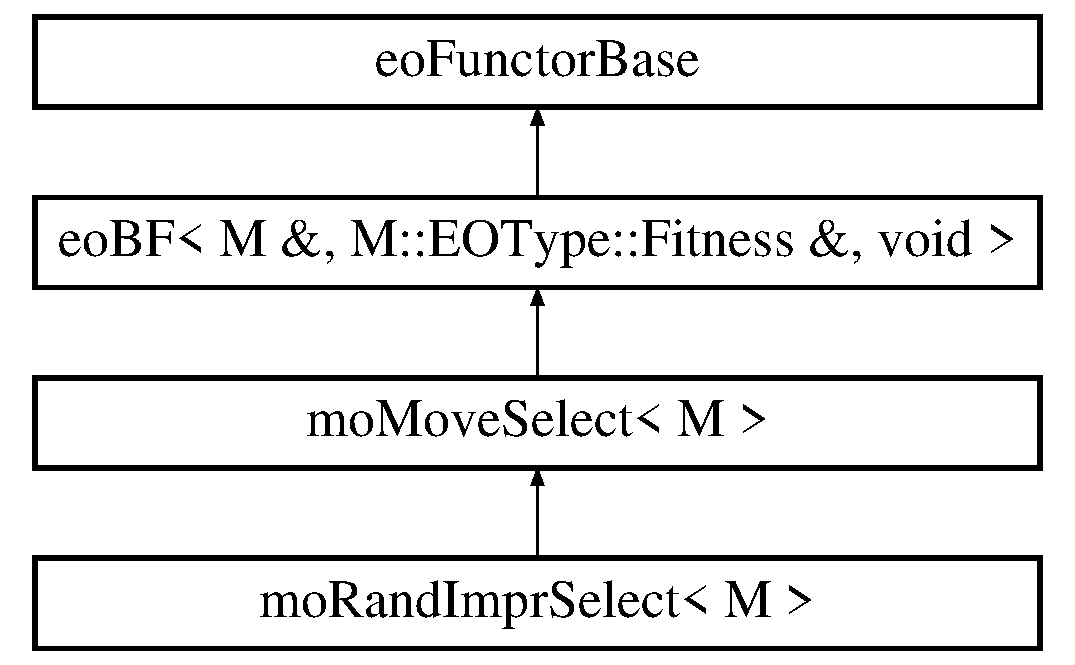
\includegraphics[height=2cm]{classmo_rand_impr_select}
\end{center}
\end{figure}
\subsection*{Public Types}
\begin{CompactItemize}
\item 
typedef M::EOType::Fitness \bf{Fitness}\label{classmo_rand_impr_select_3bff2fdb963297430543c82ffb567a5c}

\begin{CompactList}\small\item\em Alias for the fitness. \item\end{CompactList}\end{CompactItemize}
\subsection*{Public Member Functions}
\begin{CompactItemize}
\item 
void \bf{init} (const \bf{Fitness} \&\_\-fitness)
\begin{CompactList}\small\item\em Procedure which all that needs a \doxyref{mo\-Rand\-Impr\-Select}{p.}{classmo_rand_impr_select}. \item\end{CompactList}\item 
bool \bf{update} (const M \&\_\-move, const \bf{Fitness} \&\_\-fitness)
\begin{CompactList}\small\item\em Function that updates the fitness and move vectors. \item\end{CompactList}\item 
void \bf{operator()} (M \&\_\-move, \bf{Fitness} \&\_\-fitness)
\begin{CompactList}\small\item\em The move selection. \item\end{CompactList}\end{CompactItemize}
\subsection*{Private Attributes}
\begin{CompactItemize}
\item 
\bf{Fitness} \bf{initial\_\-fitness}\label{classmo_rand_impr_select_d566fa23689861b1d04257e53c71ae20}

\begin{CompactList}\small\item\em Fitness of the current solution. \item\end{CompactList}\item 
std::vector$<$ \bf{Fitness} $>$ \bf{better\_\-fitnesses}\label{classmo_rand_impr_select_220d6e3db838b11938e59bc7b29a0db6}

\begin{CompactList}\small\item\em Candidate fitnesse vector. \item\end{CompactList}\item 
std::vector$<$ M $>$ \bf{better\_\-moves}\label{classmo_rand_impr_select_8a2e7bd7d7a74d7f7402ef25737b09e1}

\begin{CompactList}\small\item\em Candidate move vector. \item\end{CompactList}\item 
bool \bf{first\-Time}\label{classmo_rand_impr_select_18f21c5ec337b45f634aaa094ad698ae}

\begin{CompactList}\small\item\em Indicate if update has been called or not. \item\end{CompactList}\end{CompactItemize}


\subsection{Detailed Description}
\subsubsection*{template$<$class M$>$ class mo\-Rand\-Impr\-Select$<$ M $>$}

One of the possible \doxyref{mo\-Move}{p.}{classmo_move} selector (\doxyref{mo\-Move\-Select}{p.}{classmo_move_select}). 

All the neighbors are considered. One of them that enables an improvment of the objective function is choosen. 



Definition at line 49 of file mo\-Rand\-Impr\-Select.h.

\subsection{Member Function Documentation}
\index{moRandImprSelect@{mo\-Rand\-Impr\-Select}!init@{init}}
\index{init@{init}!moRandImprSelect@{mo\-Rand\-Impr\-Select}}
\subsubsection{\setlength{\rightskip}{0pt plus 5cm}template$<$class M$>$ void \bf{mo\-Rand\-Impr\-Select}$<$ M $>$::init (const \bf{Fitness} \& {\em \_\-fitness})\hspace{0.3cm}{\tt  [inline, virtual]}}\label{classmo_rand_impr_select_7af99966b31aa387ecef74fd307a42e8}


Procedure which all that needs a \doxyref{mo\-Rand\-Impr\-Select}{p.}{classmo_rand_impr_select}. 

Give a value to the initialise fitness. Clean the move and fitness vectors.

\begin{Desc}
\item[Parameters:]
\begin{description}
\item[{\em \_\-fitness}]the current best fitness \end{description}
\end{Desc}


Implements \bf{mo\-Move\-Select$<$ M $>$} \doxyref{p.}{classmo_move_select_58038bd859632c1bd022d23d9792bdca}.

Definition at line 63 of file mo\-Rand\-Impr\-Select.h.

References mo\-Rand\-Impr\-Select$<$ M $>$::better\_\-fitnesses, mo\-Rand\-Impr\-Select$<$ M $>$::better\_\-moves, mo\-Rand\-Impr\-Select$<$ M $>$::first\-Time, and mo\-Rand\-Impr\-Select$<$ M $>$::initial\_\-fitness.\index{moRandImprSelect@{mo\-Rand\-Impr\-Select}!update@{update}}
\index{update@{update}!moRandImprSelect@{mo\-Rand\-Impr\-Select}}
\subsubsection{\setlength{\rightskip}{0pt plus 5cm}template$<$class M$>$ bool \bf{mo\-Rand\-Impr\-Select}$<$ M $>$::update (const M \& {\em \_\-move}, const \bf{Fitness} \& {\em \_\-fitness})\hspace{0.3cm}{\tt  [inline, virtual]}}\label{classmo_rand_impr_select_b20cfd0164266aa75960cba3c1673f69}


Function that updates the fitness and move vectors. 

if a move give a better fitness than the initial fitness, it is saved and the fitness too.

\begin{Desc}
\item[Parameters:]
\begin{description}
\item[{\em \_\-move}]a new move. \item[{\em \_\-fitness}]a new fitness associated to the new move. \end{description}
\end{Desc}
\begin{Desc}
\item[Returns:]true. \end{Desc}


Implements \bf{mo\-Move\-Select$<$ M $>$} \doxyref{p.}{classmo_move_select_5b4d3b2f030cca80c563c3db0c4af404}.

Definition at line 80 of file mo\-Rand\-Impr\-Select.h.

References mo\-Rand\-Impr\-Select$<$ M $>$::better\_\-fitnesses, mo\-Rand\-Impr\-Select$<$ M $>$::better\_\-moves, mo\-Rand\-Impr\-Select$<$ M $>$::first\-Time, and mo\-Rand\-Impr\-Select$<$ M $>$::initial\_\-fitness.\index{moRandImprSelect@{mo\-Rand\-Impr\-Select}!operator()@{operator()}}
\index{operator()@{operator()}!moRandImprSelect@{mo\-Rand\-Impr\-Select}}
\subsubsection{\setlength{\rightskip}{0pt plus 5cm}template$<$class M$>$ void \bf{mo\-Rand\-Impr\-Select}$<$ M $>$::operator() (M \& {\em \_\-move}, \bf{Fitness} \& {\em \_\-fitness})\hspace{0.3cm}{\tt  [inline]}}\label{classmo_rand_impr_select_1bc88f10830960c1d88e22e444c4e670}


The move selection. 

One the saved move is randomly chosen.

\begin{Desc}
\item[Parameters:]
\begin{description}
\item[{\em \_\-move}]the reference of the move that can be initialised by the function. \item[{\em \_\-fitness}]the reference of the fitness that can be initialised by the function. \end{description}
\end{Desc}


Definition at line 100 of file mo\-Rand\-Impr\-Select.h.

References mo\-Rand\-Impr\-Select$<$ M $>$::better\_\-fitnesses, mo\-Rand\-Impr\-Select$<$ M $>$::better\_\-moves, and mo\-Rand\-Impr\-Select$<$ M $>$::first\-Time.

The documentation for this class was generated from the following file:\begin{CompactItemize}
\item 
mo\-Rand\-Impr\-Select.h\end{CompactItemize}

\section{mo\-Rand\-Move$<$ M $>$ Class Template Reference}
\label{classmo_rand_move}\index{moRandMove@{moRandMove}}
Random move generator.  


{\tt \#include $<$mo\-Rand\-Move.h$>$}

Inheritance diagram for mo\-Rand\-Move$<$ M $>$::\begin{figure}[H]
\begin{center}
\leavevmode
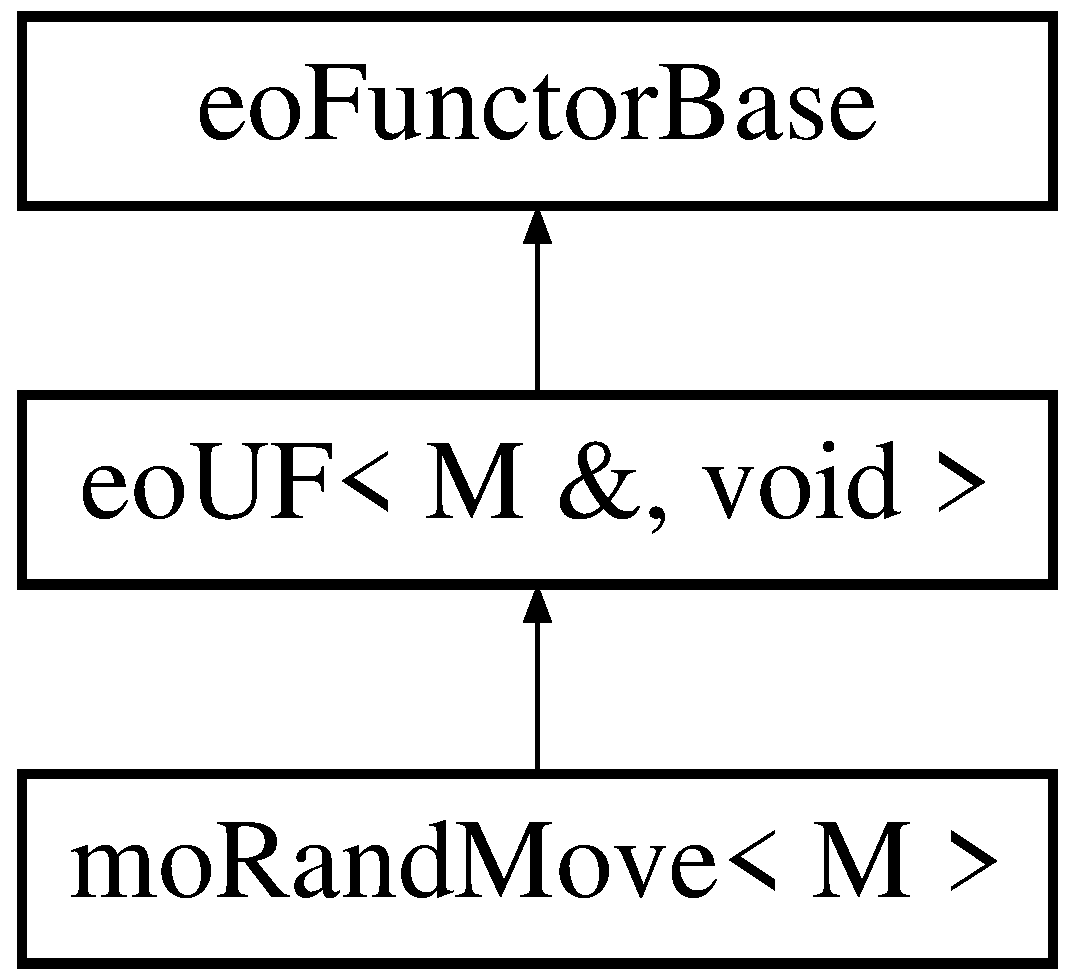
\includegraphics[height=3cm]{classmo_rand_move}
\end{center}
\end{figure}


\subsection{Detailed Description}
\subsubsection*{template$<$class M$>$ class mo\-Rand\-Move$<$ M $>$}

Random move generator. 

Only a description... An object that herits from this class needs to be designed in order to use a {\bf mo\-SA}{\rm (p.\,\pageref{classmo_s_a})}. 



Definition at line 46 of file mo\-Rand\-Move.h.

The documentation for this class was generated from the following file:\begin{CompactItemize}
\item 
mo\-Rand\-Move.h\end{CompactItemize}

\section{mo\-SA$<$ M $>$ Class Template Reference}
\label{classmo_s_a}\index{moSA@{moSA}}
Simulated Annealing (SA).  


{\tt \#include $<$mo\-SA.h$>$}

\subsection*{Public Member Functions}
\begin{CompactItemize}
\item 
\bf{mo\-SA} (\bf{mo\-Rand\-Move}$<$ M $>$ \&\_\-random\_\-move\_\-generator, \bf{mo\-Move\-Incr\-Eval}$<$ M $>$ \&\_\-incremental\_\-evaluation, \bf{mo\-Sol\-Continue}$<$ \bf{EOT} $>$ \&\_\-continue, double \_\-initial\_\-temperature, \bf{mo\-Cooling\-Schedule} \&\_\-cooling\_\-schedule, \bf{eo\-Eval\-Func}$<$ \bf{EOT} $>$ \&\_\-full\_\-evaluation)
\begin{CompactList}\small\item\em SA constructor. \item\end{CompactList}\item 
bool \bf{operator()} (\bf{EOT} \&\_\-solution)
\begin{CompactList}\small\item\em function that launches the SA algorithm. \item\end{CompactList}\end{CompactItemize}
\subsection*{Private Types}
\begin{CompactItemize}
\item 
typedef M::EOType \bf{EOT}\label{classmo_s_a_d5d64a8797bdedc7b3af7893aded0bd5}

\begin{CompactList}\small\item\em Alias for the type. \item\end{CompactList}\item 
typedef EOT::Fitness \bf{Fitness}\label{classmo_s_a_97f1a40d5ab5a0b3f878d0347b34804b}

\begin{CompactList}\small\item\em Alias for the fitness. \item\end{CompactList}\end{CompactItemize}
\subsection*{Private Attributes}
\begin{CompactItemize}
\item 
\bf{mo\-Rand\-Move}$<$ M $>$ \& \bf{random\_\-move\_\-generator}\label{classmo_s_a_92656523f556669862fcffdccea178dd}

\begin{CompactList}\small\item\em A move generator (generally randomly). \item\end{CompactList}\item 
\bf{mo\-Move\-Incr\-Eval}$<$ M $>$ \& \bf{incremental\_\-evaluation}\label{classmo_s_a_fdb49f837dc602624554279418c94bdb}

\begin{CompactList}\small\item\em A (generally) efficient evaluation function. \item\end{CompactList}\item 
\bf{mo\-Sol\-Continue}$<$ \bf{EOT} $>$ \& \bf{continu}\label{classmo_s_a_776586a839c2bbd6d12a731c12a1b748}

\begin{CompactList}\small\item\em Stopping criterion before temperature update. \item\end{CompactList}\item 
double \bf{initial\_\-temperature}\label{classmo_s_a_e07bf4ca64248e94ab85e8a1ba32aa8c}

\begin{CompactList}\small\item\em Initial temperature. \item\end{CompactList}\item 
\bf{mo\-Cooling\-Schedule} \& \bf{cooling\_\-schedule}\label{classmo_s_a_f514ae01cdfc67bf0b87d5389b3792e5}

\begin{CompactList}\small\item\em The cooling schedule. \item\end{CompactList}\item 
\bf{eo\-Eval\-Func}$<$ \bf{EOT} $>$ \& \bf{full\_\-evaluation}\label{classmo_s_a_ace30095ffc4924d84e14a0e59f7746f}

\begin{CompactList}\small\item\em A full evaluation function. \item\end{CompactList}\end{CompactItemize}


\subsection{Detailed Description}
\subsubsection*{template$<$class M$>$ class mo\-SA$<$ M $>$}

Simulated Annealing (SA). 

Class that describes a Simulated Annealing algorithm. 



Definition at line 53 of file mo\-SA.h.

\subsection{Constructor \& Destructor Documentation}
\index{moSA@{mo\-SA}!moSA@{moSA}}
\index{moSA@{moSA}!moSA@{mo\-SA}}
\subsubsection{\setlength{\rightskip}{0pt plus 5cm}template$<$class M$>$ \bf{mo\-SA}$<$ M $>$::\bf{mo\-SA} (\bf{mo\-Rand\-Move}$<$ M $>$ \& {\em \_\-random\_\-move\_\-generator}, \bf{mo\-Move\-Incr\-Eval}$<$ M $>$ \& {\em \_\-incremental\_\-evaluation}, \bf{mo\-Sol\-Continue}$<$ \bf{EOT} $>$ \& {\em \_\-continue}, double {\em \_\-initial\_\-temperature}, \bf{mo\-Cooling\-Schedule} \& {\em \_\-cooling\_\-schedule}, \bf{eo\-Eval\-Func}$<$ \bf{EOT} $>$ \& {\em \_\-full\_\-evaluation})\hspace{0.3cm}{\tt  [inline]}}\label{classmo_s_a_12e7da3a56b82daa29a30d1254da5823}


SA constructor. 

All the boxes used by a SA need to be given.

\begin{Desc}
\item[Parameters:]
\begin{description}
\item[{\em \_\-random\_\-move\_\-generator}]The move generator (generally randomly). \item[{\em \_\-incremental\_\-evaluation}]The (generally) efficient evaluation function \item[{\em \_\-continue}]The stopping criterion. \item[{\em \_\-initial\_\-temperature}]The initial temperature. \item[{\em \_\-cooling\_\-schedule}]The cooling schedule, describes how the temperature is modified. \item[{\em \_\-full\_\-evaluation}]The full evaluation function. \end{description}
\end{Desc}


Definition at line 74 of file mo\-SA.h.

\subsection{Member Function Documentation}
\index{moSA@{mo\-SA}!operator()@{operator()}}
\index{operator()@{operator()}!moSA@{mo\-SA}}
\subsubsection{\setlength{\rightskip}{0pt plus 5cm}template$<$class M$>$ bool \bf{mo\-SA}$<$ M $>$::operator() (\bf{EOT} \& {\em \_\-solution})\hspace{0.3cm}{\tt  [inline, virtual]}}\label{classmo_s_a_bea8176b0c05a96696b2ab29d3f3c544}


function that launches the SA algorithm. 

As a \doxyref{mo\-TS}{p.}{classmo_t_s} or a \doxyref{mo\-HC}{p.}{classmo_h_c}, the SA can be used for HYBRIDATION in an evolutionary algorithm.

\begin{Desc}
\item[Parameters:]
\begin{description}
\item[{\em \_\-solution}]A solution to improve. \end{description}
\end{Desc}
\begin{Desc}
\item[Returns:]TRUE. \end{Desc}


Implements \bf{eo\-UF$<$ M::EOType \&, bool $>$}.

Definition at line 89 of file mo\-SA.h.

References mo\-SA$<$ M $>$::continu, mo\-SA$<$ M $>$::cooling\_\-schedule, mo\-SA$<$ M $>$::full\_\-evaluation, mo\-SA$<$ M $>$::incremental\_\-evaluation, mo\-SA$<$ M $>$::initial\_\-temperature, mo\-SA$<$ M $>$::random\_\-move\_\-generator, and eo\-Rng::uniform().

The documentation for this class was generated from the following file:\begin{CompactItemize}
\item 
mo\-SA.h\end{CompactItemize}

\section{mo\-Simple\-Move\-Tabu\-List$<$ M $>$ Class Template Reference}
\label{classmo_simple_move_tabu_list}\index{moSimpleMoveTabuList@{moSimpleMoveTabuList}}
Class describing a move tabu list with a limited memory.  


{\tt \#include $<$mo\-Simple\-Move\-Tabu\-List.h$>$}

Inheritance diagram for mo\-Simple\-Move\-Tabu\-List$<$ M $>$::\begin{figure}[H]
\begin{center}
\leavevmode
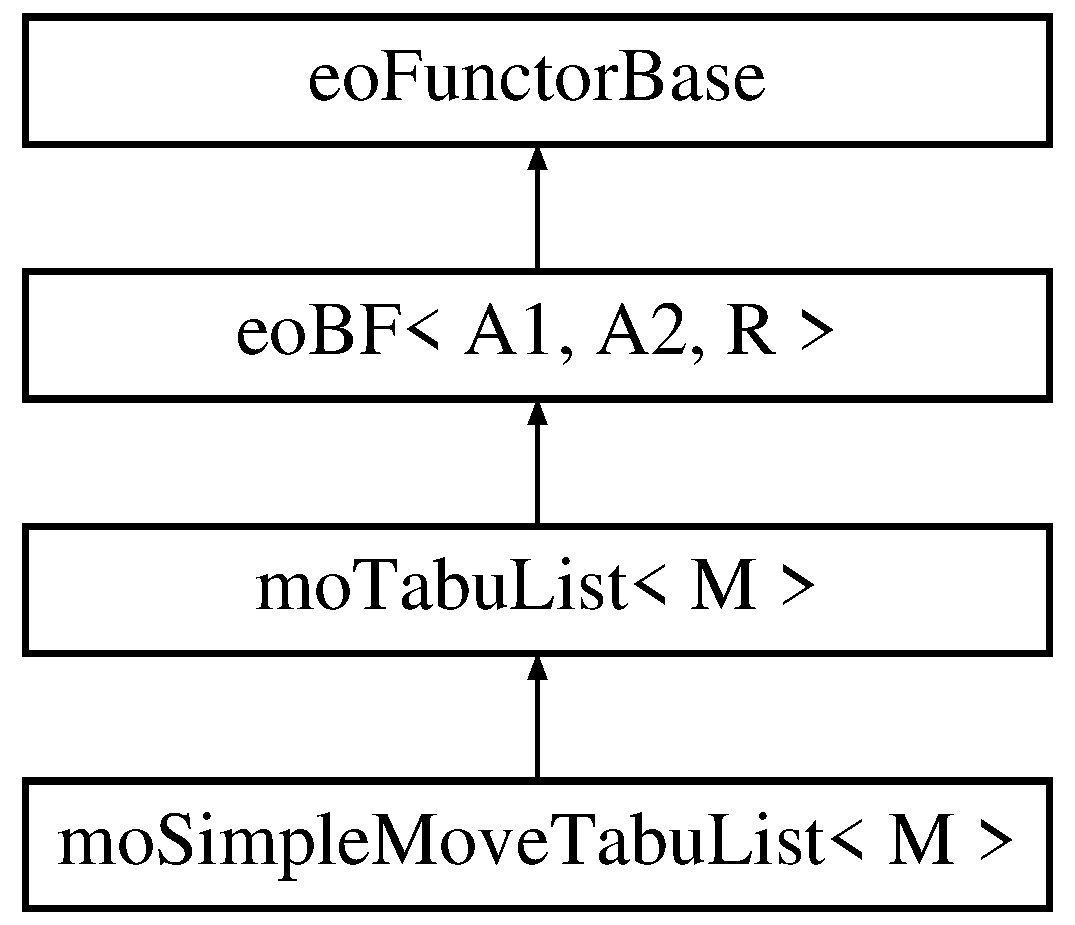
\includegraphics[height=4cm]{classmo_simple_move_tabu_list}
\end{center}
\end{figure}
\subsection*{Public Types}
\begin{CompactItemize}
\item 
typedef M::EOType \bf{EOT}\label{classmo_simple_move_tabu_list_91286ff3ba6b1e9e1db9e4fdade2edb7}

\begin{CompactList}\small\item\em Alias for the type. \item\end{CompactList}\item 
typedef std::list$<$ M $>$::iterator \bf{move\-Iterator}\label{classmo_simple_move_tabu_list_4ca9387c0a20bb9f4142682cbfee26bf}

\begin{CompactList}\small\item\em Alias for an iterator of a move list. \item\end{CompactList}\end{CompactItemize}
\subsection*{Public Member Functions}
\begin{CompactItemize}
\item 
\bf{mo\-Simple\-Move\-Tabu\-List} (unsigned int \_\-memory\_\-maximum\_\-size)\label{classmo_simple_move_tabu_list_c27e7fabe1370ea65f56981c5cbc1769}

\begin{CompactList}\small\item\em Constructor. \item\end{CompactList}\item 
bool \bf{operator()} (const M \&\_\-move, const \bf{EOT} \&\_\-solution)
\begin{CompactList}\small\item\em \doxyref{Function} that indicates if, in a given state, the \_\-move is tabu or not. \item\end{CompactList}\item 
void \bf{add} (const M \&\_\-move, const \bf{EOT} \&\_\-solution)
\begin{CompactList}\small\item\em Procedure to add a move in the tabu list. \item\end{CompactList}\item 
void \bf{update} ()
\begin{CompactList}\small\item\em Procedure that updates the tabu list content. \item\end{CompactList}\item 
void \bf{init} ()
\begin{CompactList}\small\item\em Procedure which initialises the tabu list. \item\end{CompactList}\end{CompactItemize}
\subsection*{Private Member Functions}
\begin{CompactItemize}
\item 
void \bf{remove\-Move} (const M \&\_\-move)
\begin{CompactList}\small\item\em Procedure that removes a given move from the tabu list (if it is into, else do nothing). \item\end{CompactList}\end{CompactItemize}
\subsection*{Private Attributes}
\begin{CompactItemize}
\item 
unsigned int \bf{memory\_\-maximum\_\-size}\label{classmo_simple_move_tabu_list_fea7fe7c62a6da9b8f087a2732f44251}

\begin{CompactList}\small\item\em The maximum size of the tabu list. \item\end{CompactList}\item 
unsigned int \bf{memory\_\-size}\label{classmo_simple_move_tabu_list_defd20fe6d0d51fdaedbc5b95018aea7}

\begin{CompactList}\small\item\em The current size of the tabu list. \item\end{CompactList}\item 
std::list$<$ M $>$ \bf{tabu\-List}\label{classmo_simple_move_tabu_list_d91bc838361524720616b44eda9b2c3a}

\begin{CompactList}\small\item\em The move tabu list. \item\end{CompactList}\end{CompactItemize}


\subsection{Detailed Description}
\subsubsection*{template$<$class M$>$ class mo\-Simple\-Move\-Tabu\-List$<$ M $>$}

Class describing a move tabu list with a limited memory. 



Definition at line 46 of file mo\-Simple\-Move\-Tabu\-List.h.

\subsection{Member Function Documentation}
\index{moSimpleMoveTabuList@{mo\-Simple\-Move\-Tabu\-List}!operator()@{operator()}}
\index{operator()@{operator()}!moSimpleMoveTabuList@{mo\-Simple\-Move\-Tabu\-List}}
\subsubsection{\setlength{\rightskip}{0pt plus 5cm}template$<$class M$>$ bool \bf{mo\-Simple\-Move\-Tabu\-List}$<$ M $>$::operator() (const M \& {\em \_\-move}, const \bf{EOT} \& {\em \_\-solution})\hspace{0.3cm}{\tt  [inline]}}\label{classmo_simple_move_tabu_list_8d38f296f3d7721025820f16f25fcf7e}


\doxyref{Function} that indicates if, in a given state, the \_\-move is tabu or not. 

\begin{Desc}
\item[Parameters:]
\begin{description}
\item[{\em \_\-move}]A given \doxyref{mo\-Move}{p.}{classmo_move}. \item[{\em \_\-solution}]A solution. \end{description}
\end{Desc}
\begin{Desc}
\item[Returns:]true or false. \end{Desc}


Definition at line 69 of file mo\-Simple\-Move\-Tabu\-List.h.

References mo\-Simple\-Move\-Tabu\-List$<$ M $>$::tabu\-List.\index{moSimpleMoveTabuList@{mo\-Simple\-Move\-Tabu\-List}!add@{add}}
\index{add@{add}!moSimpleMoveTabuList@{mo\-Simple\-Move\-Tabu\-List}}
\subsubsection{\setlength{\rightskip}{0pt plus 5cm}template$<$class M$>$ void \bf{mo\-Simple\-Move\-Tabu\-List}$<$ M $>$::add (const M \& {\em \_\-move}, const \bf{EOT} \& {\em \_\-solution})\hspace{0.3cm}{\tt  [inline, virtual]}}\label{classmo_simple_move_tabu_list_e6c0835fbfab2bdc63097cf2fd5328aa}


Procedure to add a move in the tabu list. 

The two parameters have not to be modified so they are constant parameters.

\begin{Desc}
\item[Parameters:]
\begin{description}
\item[{\em \_\-move}]a new tabu move. \item[{\em \_\-solution}]the origianl solution associated to this move. \end{description}
\end{Desc}


Implements \bf{mo\-Tabu\-List$<$ M $>$} \doxyref{p.}{classmo_tabu_list_55204939b6d67b6d37b4af725d70cf6d}.

Definition at line 86 of file mo\-Simple\-Move\-Tabu\-List.h.

References mo\-Simple\-Move\-Tabu\-List$<$ M $>$::memory\_\-maximum\_\-size, mo\-Simple\-Move\-Tabu\-List$<$ M $>$::memory\_\-size, mo\-Simple\-Move\-Tabu\-List$<$ M $>$::remove\-Move(), and mo\-Simple\-Move\-Tabu\-List$<$ M $>$::tabu\-List.\index{moSimpleMoveTabuList@{mo\-Simple\-Move\-Tabu\-List}!update@{update}}
\index{update@{update}!moSimpleMoveTabuList@{mo\-Simple\-Move\-Tabu\-List}}
\subsubsection{\setlength{\rightskip}{0pt plus 5cm}template$<$class M$>$ void \bf{mo\-Simple\-Move\-Tabu\-List}$<$ M $>$::update ()\hspace{0.3cm}{\tt  [inline, virtual]}}\label{classmo_simple_move_tabu_list_96cffc8118456ed762b07b9fc0e0679f}


Procedure that updates the tabu list content. 

Generally, a counter associated to each saved move is decreased by one. 

Implements \bf{mo\-Tabu\-List$<$ M $>$} \doxyref{p.}{classmo_tabu_list_a2e5d1132f064093c8ed57046405f5ca}.

Definition at line 110 of file mo\-Simple\-Move\-Tabu\-List.h.\index{moSimpleMoveTabuList@{mo\-Simple\-Move\-Tabu\-List}!init@{init}}
\index{init@{init}!moSimpleMoveTabuList@{mo\-Simple\-Move\-Tabu\-List}}
\subsubsection{\setlength{\rightskip}{0pt plus 5cm}template$<$class M$>$ void \bf{mo\-Simple\-Move\-Tabu\-List}$<$ M $>$::init ()\hspace{0.3cm}{\tt  [inline, virtual]}}\label{classmo_simple_move_tabu_list_b91ae9971be30769757d1ad92c6009dc}


Procedure which initialises the tabu list. 

Can be useful if the data structure needs to be allocated before being used. 

Implements \bf{mo\-Tabu\-List$<$ M $>$} \doxyref{p.}{classmo_tabu_list_0a06c459d56e8e2b408a8f3c6aec4e57}.

Definition at line 115 of file mo\-Simple\-Move\-Tabu\-List.h.\index{moSimpleMoveTabuList@{mo\-Simple\-Move\-Tabu\-List}!removeMove@{removeMove}}
\index{removeMove@{removeMove}!moSimpleMoveTabuList@{mo\-Simple\-Move\-Tabu\-List}}
\subsubsection{\setlength{\rightskip}{0pt plus 5cm}template$<$class M$>$ void \bf{mo\-Simple\-Move\-Tabu\-List}$<$ M $>$::remove\-Move (const M \& {\em \_\-move})\hspace{0.3cm}{\tt  [inline, private]}}\label{classmo_simple_move_tabu_list_922ac2e3c45cbb94698517265be95de5}


Procedure that removes a given move from the tabu list (if it is into, else do nothing). 

\begin{Desc}
\item[Parameters:]
\begin{description}
\item[{\em \_\-move}]A given \doxyref{mo\-Move}{p.}{classmo_move}. \end{description}
\end{Desc}


Definition at line 126 of file mo\-Simple\-Move\-Tabu\-List.h.

References mo\-Simple\-Move\-Tabu\-List$<$ M $>$::tabu\-List.

Referenced by mo\-Simple\-Move\-Tabu\-List$<$ M $>$::add().

The documentation for this class was generated from the following file:\begin{CompactItemize}
\item 
mo\-Simple\-Move\-Tabu\-List.h\end{CompactItemize}

\section{moSimpleSolutionTabuList$<$ M $>$ Class Template Reference}
\label{classmo_simple_solution_tabu_list}\index{moSimpleSolutionTabuList@{moSimpleSolutionTabuList}}
Class describing a solution tabu list with limited length.  


{\tt \#include $<$moSimpleSolutionTabuList.h$>$}

Inheritance diagram for moSimpleSolutionTabuList$<$ M $>$::\begin{figure}[H]
\begin{center}
\leavevmode
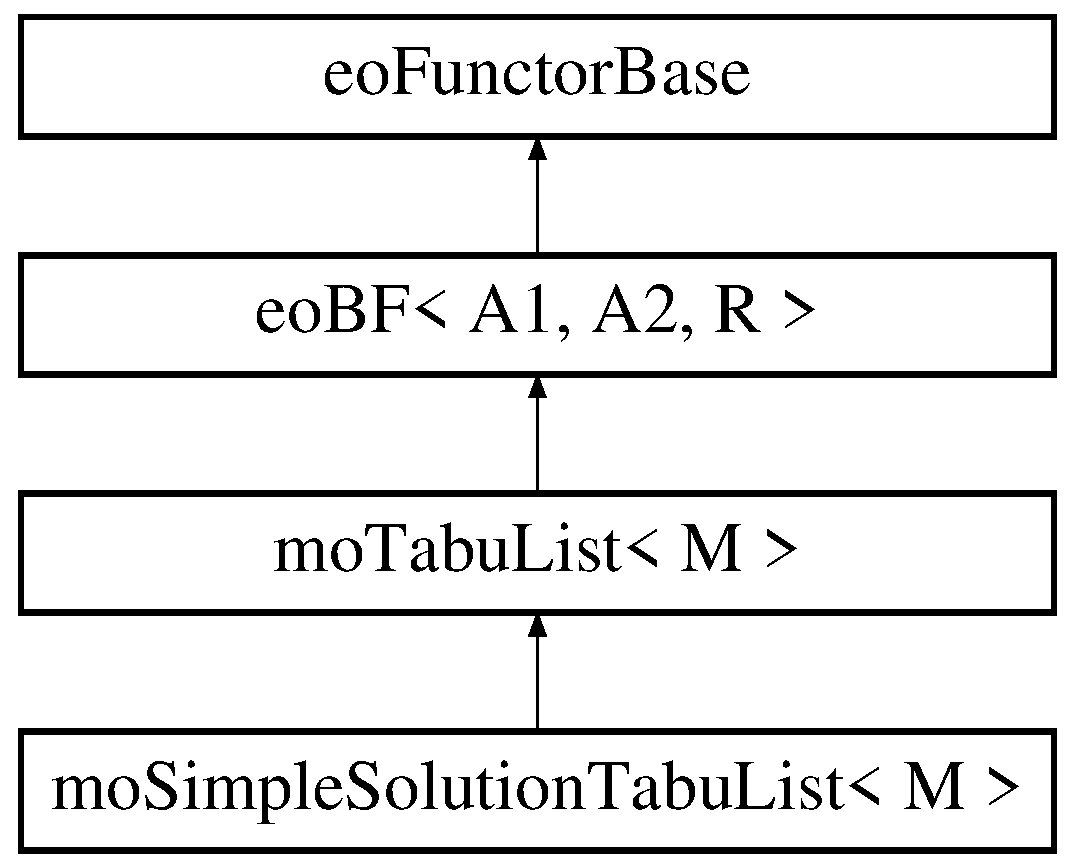
\includegraphics[height=4cm]{classmo_simple_solution_tabu_list}
\end{center}
\end{figure}
\subsection*{Public Types}
\begin{CompactItemize}
\item 
typedef M::EOType {\bf EOT}\label{classmo_simple_solution_tabu_list_881060871a6b49e5e8554c5df85176d9}

\begin{CompactList}\small\item\em Alias for the type. \item\end{CompactList}\item 
typedef std::list$<$ {\bf EOT} $>$::iterator {\bf solutionIterator}\label{classmo_simple_solution_tabu_list_3438db9ed9e1a94a24c418d8cbadec54}

\begin{CompactList}\small\item\em Alias for an iterator of a solution list. \item\end{CompactList}\end{CompactItemize}
\subsection*{Public Member Functions}
\begin{CompactItemize}
\item 
{\bf moSimpleSolutionTabuList} (unsigned int \_\-memory\_\-maximum\_\-size)
\begin{CompactList}\small\item\em Constructor. \item\end{CompactList}\item 
bool {\bf operator()} (const M \&\_\-move, const {\bf EOT} \&\_\-solution)
\begin{CompactList}\small\item\em {\bf Function} that indicates if, in a given state, the \_\-move is tabu or not. \item\end{CompactList}\item 
void {\bf add} (const M \&\_\-move, const {\bf EOT} \&\_\-solution)
\begin{CompactList}\small\item\em Procedure to add a move in the tabu list. \item\end{CompactList}\item 
void {\bf update} ()
\begin{CompactList}\small\item\em Procedure that updates the tabu list content. \item\end{CompactList}\item 
void {\bf init} ()
\begin{CompactList}\small\item\em Procedure which initialises the tabu list. \item\end{CompactList}\end{CompactItemize}
\subsection*{Private Member Functions}
\begin{CompactItemize}
\item 
void {\bf removeSolution} (const {\bf EOT} \&\_\-solution)
\begin{CompactList}\small\item\em Procedure that removes a given solution from the tabu list (if it is into, else does nothing). \item\end{CompactList}\end{CompactItemize}
\subsection*{Private Attributes}
\begin{CompactItemize}
\item 
unsigned int {\bf memory\_\-maximum\_\-size}\label{classmo_simple_solution_tabu_list_06631e7b9a2511e3c11540aa14b9e636}

\begin{CompactList}\small\item\em The maximum size of the tabu list. \item\end{CompactList}\item 
unsigned int {\bf memory\_\-size}\label{classmo_simple_solution_tabu_list_0d54e6b0af0e6088aafae596392c9490}

\begin{CompactList}\small\item\em The current size of the tabu list. \item\end{CompactList}\item 
std::list$<$ {\bf EOT} $>$ {\bf tabuList}\label{classmo_simple_solution_tabu_list_75df9cd683528d3722d02bac407b710b}

\begin{CompactList}\small\item\em The solution tabu list. \item\end{CompactList}\end{CompactItemize}


\subsection{Detailed Description}
\subsubsection*{template$<$class M$>$ class moSimpleSolutionTabuList$<$ M $>$}

Class describing a solution tabu list with limited length. 

Definition at line 46 of file moSimpleSolutionTabuList.h.

\subsection{Constructor \& Destructor Documentation}
\index{moSimpleSolutionTabuList@{moSimpleSolutionTabuList}!moSimpleSolutionTabuList@{moSimpleSolutionTabuList}}
\index{moSimpleSolutionTabuList@{moSimpleSolutionTabuList}!moSimpleSolutionTabuList@{moSimpleSolutionTabuList}}
\subsubsection{\setlength{\rightskip}{0pt plus 5cm}template$<$class M$>$ {\bf moSimpleSolutionTabuList}$<$ M $>$::{\bf moSimpleSolutionTabuList} (unsigned int {\em \_\-memory\_\-maximum\_\-size})\hspace{0.3cm}{\tt  [inline]}}\label{classmo_simple_solution_tabu_list_8499bf947de47519d155e9e45f815d41}


Constructor. 

\begin{Desc}
\item[Parameters:]
\begin{description}
\item[{\em \_\-memory\_\-maximum\_\-size}]The maximum size of the solution tabu list. \end{description}
\end{Desc}


Definition at line 60 of file moSimpleSolutionTabuList.h.

\subsection{Member Function Documentation}
\index{moSimpleSolutionTabuList@{moSimpleSolutionTabuList}!operator()@{operator()}}
\index{operator()@{operator()}!moSimpleSolutionTabuList@{moSimpleSolutionTabuList}}
\subsubsection{\setlength{\rightskip}{0pt plus 5cm}template$<$class M$>$ bool {\bf moSimpleSolutionTabuList}$<$ M $>$::operator() (const M \& {\em \_\-move}, const {\bf EOT} \& {\em \_\-solution})\hspace{0.3cm}{\tt  [inline]}}\label{classmo_simple_solution_tabu_list_9052858ae3e6765cbe4c344bdae6c692}


{\bf Function} that indicates if, in a given state, the \_\-move is tabu or not. 

\begin{Desc}
\item[Parameters:]
\begin{description}
\item[{\em \_\-move}]A given \doxyref{moMove}{p.}{classmo_move}. \item[{\em \_\-solution}]A solution. \end{description}
\end{Desc}
\begin{Desc}
\item[Returns:]true or false. \end{Desc}


Definition at line 69 of file moSimpleSolutionTabuList.h.

References moSimpleSolutionTabuList$<$ M $>$::tabuList.\index{moSimpleSolutionTabuList@{moSimpleSolutionTabuList}!add@{add}}
\index{add@{add}!moSimpleSolutionTabuList@{moSimpleSolutionTabuList}}
\subsubsection{\setlength{\rightskip}{0pt plus 5cm}template$<$class M$>$ void {\bf moSimpleSolutionTabuList}$<$ M $>$::add (const M \& {\em \_\-move}, const {\bf EOT} \& {\em \_\-solution})\hspace{0.3cm}{\tt  [inline, virtual]}}\label{classmo_simple_solution_tabu_list_58ae13e7642c429ea51ff679a932aceb}


Procedure to add a move in the tabu list. 

The two parameters have not to be modified so they are constant parameters.

\begin{Desc}
\item[Parameters:]
\begin{description}
\item[{\em \_\-move}]a new tabu move. \item[{\em \_\-solution}]the origianl solution associated to this move. \end{description}
\end{Desc}


Implements {\bf moTabuList$<$ M $>$} \doxyref{}{p.}{classmo_tabu_list_55204939b6d67b6d37b4af725d70cf6d}.

Definition at line 89 of file moSimpleSolutionTabuList.h.

References moSimpleSolutionTabuList$<$ M $>$::memory\_\-maximum\_\-size, moSimpleSolutionTabuList$<$ M $>$::memory\_\-size, moSimpleSolutionTabuList$<$ M $>$::removeSolution(), and moSimpleSolutionTabuList$<$ M $>$::tabuList.\index{moSimpleSolutionTabuList@{moSimpleSolutionTabuList}!update@{update}}
\index{update@{update}!moSimpleSolutionTabuList@{moSimpleSolutionTabuList}}
\subsubsection{\setlength{\rightskip}{0pt plus 5cm}template$<$class M$>$ void {\bf moSimpleSolutionTabuList}$<$ M $>$::update ()\hspace{0.3cm}{\tt  [inline, virtual]}}\label{classmo_simple_solution_tabu_list_91b8b01dba7ffea8b63765d931e56f56}


Procedure that updates the tabu list content. 

Generally, a counter associated to each saved move is decreased by one. 

Implements {\bf moTabuList$<$ M $>$} \doxyref{}{p.}{classmo_tabu_list_a2e5d1132f064093c8ed57046405f5ca}.

Definition at line 115 of file moSimpleSolutionTabuList.h.\index{moSimpleSolutionTabuList@{moSimpleSolutionTabuList}!init@{init}}
\index{init@{init}!moSimpleSolutionTabuList@{moSimpleSolutionTabuList}}
\subsubsection{\setlength{\rightskip}{0pt plus 5cm}template$<$class M$>$ void {\bf moSimpleSolutionTabuList}$<$ M $>$::init ()\hspace{0.3cm}{\tt  [inline, virtual]}}\label{classmo_simple_solution_tabu_list_d5645c39fec71a6110a2cbccbb08b816}


Procedure which initialises the tabu list. 

Can be useful if the data structure needs to be allocated before being used. 

Implements {\bf moTabuList$<$ M $>$} \doxyref{}{p.}{classmo_tabu_list_0a06c459d56e8e2b408a8f3c6aec4e57}.

Definition at line 120 of file moSimpleSolutionTabuList.h.\index{moSimpleSolutionTabuList@{moSimpleSolutionTabuList}!removeSolution@{removeSolution}}
\index{removeSolution@{removeSolution}!moSimpleSolutionTabuList@{moSimpleSolutionTabuList}}
\subsubsection{\setlength{\rightskip}{0pt plus 5cm}template$<$class M$>$ void {\bf moSimpleSolutionTabuList}$<$ M $>$::removeSolution (const {\bf EOT} \& {\em \_\-solution})\hspace{0.3cm}{\tt  [inline, private]}}\label{classmo_simple_solution_tabu_list_e4a57001a201e1fb7446902381a7ac7d}


Procedure that removes a given solution from the tabu list (if it is into, else does nothing). 

\begin{Desc}
\item[Parameters:]
\begin{description}
\item[{\em \_\-solution}]A given solution. \end{description}
\end{Desc}


Definition at line 131 of file moSimpleSolutionTabuList.h.

References moSimpleSolutionTabuList$<$ M $>$::tabuList.

Referenced by moSimpleSolutionTabuList$<$ M $>$::add().

The documentation for this class was generated from the following file:\begin{CompactItemize}
\item 
moSimpleSolutionTabuList.h\end{CompactItemize}

\section{mo\-Sol\-Continue$<$ EOT $>$ Class Template Reference}
\label{classmo_sol_continue}\index{moSolContinue@{moSolContinue}}
Class that describes a stop criterion for a solution-based heuristic.  


{\tt \#include $<$mo\-Sol\-Continue.h$>$}

Inheritance diagram for mo\-Sol\-Continue$<$ EOT $>$::\begin{figure}[H]
\begin{center}
\leavevmode
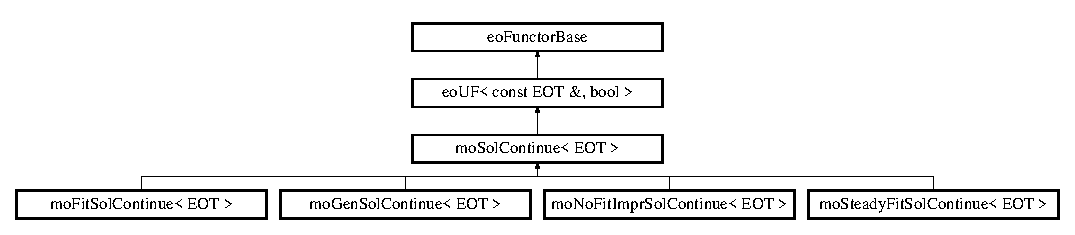
\includegraphics[height=1.35266cm]{classmo_sol_continue}
\end{center}
\end{figure}
\subsection*{Public Member Functions}
\begin{CompactItemize}
\item 
virtual void \bf{init} ()=0
\begin{CompactList}\small\item\em Procedure which initialises all that the stop criterion needs. \item\end{CompactList}\end{CompactItemize}


\subsection{Detailed Description}
\subsubsection*{template$<$class EOT$>$ class mo\-Sol\-Continue$<$ EOT $>$}

Class that describes a stop criterion for a solution-based heuristic. 

It allows to add an initialisation procedure to an object that is a unary function (eo\-UF). 



Definition at line 48 of file mo\-Sol\-Continue.h.

\subsection{Member Function Documentation}
\index{moSolContinue@{mo\-Sol\-Continue}!init@{init}}
\index{init@{init}!moSolContinue@{mo\-Sol\-Continue}}
\subsubsection{\setlength{\rightskip}{0pt plus 5cm}template$<$class EOT$>$ virtual void \bf{mo\-Sol\-Continue}$<$ EOT $>$::init ()\hspace{0.3cm}{\tt  [pure virtual]}}\label{classmo_sol_continue_064dc966a210f4ffb9515be3f03ca4c7}


Procedure which initialises all that the stop criterion needs. 

Generally, it allocates some data structures or initialises some counters. 

Implemented in \bf{mo\-Fit\-Sol\-Continue$<$ EOT $>$} \doxyref{p.}{classmo_fit_sol_continue_670bd895b4edfcd3aebb40d2295d7f7c}, \bf{mo\-Gen\-Sol\-Continue$<$ EOT $>$} \doxyref{p.}{classmo_gen_sol_continue_6c5db8182157584b56507cc9075602d4}, \bf{mo\-No\-Fit\-Impr\-Sol\-Continue$<$ EOT $>$} \doxyref{p.}{classmo_no_fit_impr_sol_continue_21641c0a38a4501baae6133cbc591de4}, and \bf{mo\-Steady\-Fit\-Sol\-Continue$<$ EOT $>$} \doxyref{p.}{classmo_steady_fit_sol_continue_87563493addc8e4b58982c55a67179b9}.

The documentation for this class was generated from the following file:\begin{CompactItemize}
\item 
mo\-Sol\-Continue.h\end{CompactItemize}

\section{moSteadyFitSolContinue$<$ EOT $>$ Class Template Reference}
\label{classmo_steady_fit_sol_continue}\index{moSteadyFitSolContinue@{moSteadyFitSolContinue}}
One possible stopping criterion for a solution-based heuristic.  


{\tt \#include $<$moSteadyFitSolContinue.h$>$}

Inheritance diagram for moSteadyFitSolContinue$<$ EOT $>$::\begin{figure}[H]
\begin{center}
\leavevmode
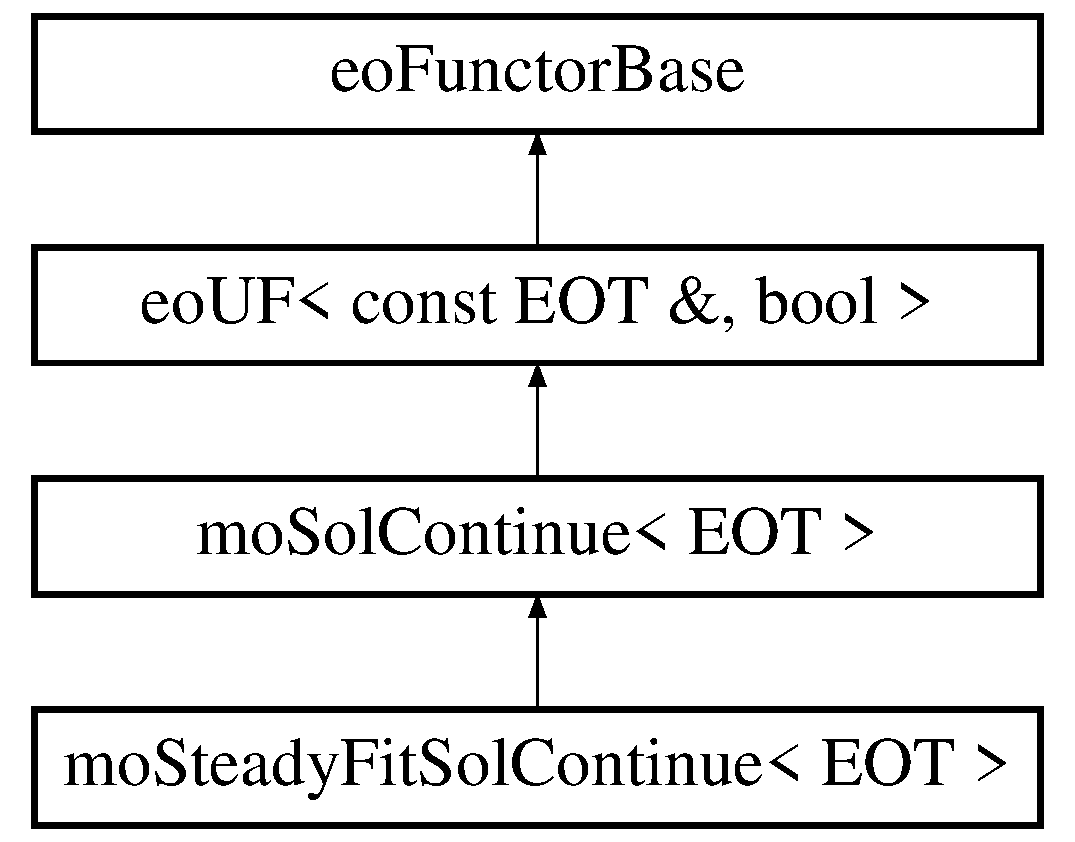
\includegraphics[height=4cm]{classmo_steady_fit_sol_continue}
\end{center}
\end{figure}
\subsection*{Public Types}
\begin{CompactItemize}
\item 
typedef EOT::Fitness {\bf Fitness}\label{classmo_steady_fit_sol_continue_c289721abbbafe50f6e3b8305dd31007}

\begin{CompactList}\small\item\em Alias for the fitness. \item\end{CompactList}\end{CompactItemize}
\subsection*{Public Member Functions}
\begin{CompactItemize}
\item 
{\bf moSteadyFitSolContinue} (unsigned int \_\-maxNumberOfIterations, unsigned int \_\-maxNumberOfIterationWithoutImprovement)
\begin{CompactList}\small\item\em Basic constructor. \item\end{CompactList}\item 
bool {\bf operator()} (const EOT \&\_\-solution)
\begin{CompactList}\small\item\em {\bf Function} that activates the stopping criterion. \item\end{CompactList}\item 
void {\bf init} ()
\begin{CompactList}\small\item\em Procedure which allows to initialise the stuff needed. \item\end{CompactList}\end{CompactItemize}
\subsection*{Private Attributes}
\begin{CompactItemize}
\item 
unsigned int {\bf maxNumberOfIterations}\label{classmo_steady_fit_sol_continue_36b43c2a252887ad027165ac32393fe8}

\begin{CompactList}\small\item\em Maximum number of iterations before considering the fitness. \item\end{CompactList}\item 
unsigned int {\bf maxNumberOfIterationsWithoutImprovement}\label{classmo_steady_fit_sol_continue_cde593c09f497a5fa66ff62732544f40}

\begin{CompactList}\small\item\em Maximum number of iterations without improvement allowed. \item\end{CompactList}\item 
bool {\bf maxNumberOfIterationsReached}\label{classmo_steady_fit_sol_continue_7d88c0eb91b2a12121ba1c3ae9139887}

\begin{CompactList}\small\item\em Flag that indicates that the maxNumberIteration have been reached. \item\end{CompactList}\item 
bool {\bf firstFitnessSaved}\label{classmo_steady_fit_sol_continue_025bf2789e470fdde989eee9121035c3}

\begin{CompactList}\small\item\em Flag that this is the first time that the fitness is used. \item\end{CompactList}\item 
{\bf Fitness} {\bf fitness}\label{classmo_steady_fit_sol_continue_a5c62e7049b36f6e71e92b559568c09e}

\begin{CompactList}\small\item\em Current Fitness. \item\end{CompactList}\item 
unsigned int {\bf counter}\label{classmo_steady_fit_sol_continue_245c9099a2c40dfc4f34b3ff216d13ce}

\begin{CompactList}\small\item\em The iteration couter. \item\end{CompactList}\end{CompactItemize}


\subsection{Detailed Description}
\subsubsection*{template$<$class EOT$>$ class moSteadyFitSolContinue$<$ EOT $>$}

One possible stopping criterion for a solution-based heuristic. 

The stop criterion corresponds to a maximum number of iterations without improvement (after a minimum number of iterations). 

Definition at line 46 of file moSteadyFitSolContinue.h.

\subsection{Constructor \& Destructor Documentation}
\index{moSteadyFitSolContinue@{moSteadyFitSolContinue}!moSteadyFitSolContinue@{moSteadyFitSolContinue}}
\index{moSteadyFitSolContinue@{moSteadyFitSolContinue}!moSteadyFitSolContinue@{moSteadyFitSolContinue}}
\subsubsection{\setlength{\rightskip}{0pt plus 5cm}template$<$class EOT$>$ {\bf moSteadyFitSolContinue}$<$ EOT $>$::{\bf moSteadyFitSolContinue} (unsigned int {\em \_\-maxNumberOfIterations}, unsigned int {\em \_\-maxNumberOfIterationWithoutImprovement})\hspace{0.3cm}{\tt  [inline]}}\label{classmo_steady_fit_sol_continue_c5e0e998b73e3a48ca3e87f4f816569b}


Basic constructor. 

\begin{Desc}
\item[Parameters:]
\begin{description}
\item[{\em \_\-maxNumberOfIterations}]The number of iterations to reach before looking for the fitness. \item[{\em \_\-maxNumberOfIterationWithoutImprovement}]The number of iterations without fitness improvement to reach for stop. \end{description}
\end{Desc}


Definition at line 58 of file moSteadyFitSolContinue.h.

\subsection{Member Function Documentation}
\index{moSteadyFitSolContinue@{moSteadyFitSolContinue}!operator()@{operator()}}
\index{operator()@{operator()}!moSteadyFitSolContinue@{moSteadyFitSolContinue}}
\subsubsection{\setlength{\rightskip}{0pt plus 5cm}template$<$class EOT$>$ bool {\bf moSteadyFitSolContinue}$<$ EOT $>$::operator() (const EOT \& {\em \_\-solution})\hspace{0.3cm}{\tt  [inline, virtual]}}\label{classmo_steady_fit_sol_continue_f7432bccb768d50a2fef248c2b174904}


{\bf Function} that activates the stopping criterion. 

Indicates if the fitness has not been improved since a number of iterations (after a minimum of iterations).

\begin{Desc}
\item[Parameters:]
\begin{description}
\item[{\em \_\-solution}]the current solution. \end{description}
\end{Desc}
\begin{Desc}
\item[Returns:]true or false. \end{Desc}


Implements {\bf eoUF$<$ const EOT \&, bool $>$}.

Definition at line 70 of file moSteadyFitSolContinue.h.

References moSteadyFitSolContinue$<$ EOT $>$::counter, moSteadyFitSolContinue$<$ EOT $>$::firstFitnessSaved, moSteadyFitSolContinue$<$ EOT $>$::fitness, moSteadyFitSolContinue$<$ EOT $>$::maxNumberOfIterations, moSteadyFitSolContinue$<$ EOT $>$::maxNumberOfIterationsReached, and moSteadyFitSolContinue$<$ EOT $>$::maxNumberOfIterationsWithoutImprovement.\index{moSteadyFitSolContinue@{moSteadyFitSolContinue}!init@{init}}
\index{init@{init}!moSteadyFitSolContinue@{moSteadyFitSolContinue}}
\subsubsection{\setlength{\rightskip}{0pt plus 5cm}template$<$class EOT$>$ void {\bf moSteadyFitSolContinue}$<$ EOT $>$::init ()\hspace{0.3cm}{\tt  [inline, virtual]}}\label{classmo_steady_fit_sol_continue_87563493addc8e4b58982c55a67179b9}


Procedure which allows to initialise the stuff needed. 

It can be also used to reinitialize the counter all the needed things. 

Implements {\bf moSolContinue$<$ EOT $>$} \doxyref{}{p.}{classmo_sol_continue_064dc966a210f4ffb9515be3f03ca4c7}.

Definition at line 114 of file moSteadyFitSolContinue.h.

References moSteadyFitSolContinue$<$ EOT $>$::counter, moSteadyFitSolContinue$<$ EOT $>$::firstFitnessSaved, and moSteadyFitSolContinue$<$ EOT $>$::maxNumberOfIterationsReached.

The documentation for this class was generated from the following file:\begin{CompactItemize}
\item 
moSteadyFitSolContinue.h\end{CompactItemize}

\section{mo\-Tabu\-List$<$ M $>$ Class Template Reference}
\label{classmo_tabu_list}\index{moTabuList@{moTabuList}}
Class describing a tabu list that a {\bf mo\-TS}{\rm (p.\,\pageref{classmo_t_s})} uses.  


{\tt \#include $<$mo\-Tabu\-List.h$>$}

Inheritance diagram for mo\-Tabu\-List$<$ M $>$::\begin{figure}[H]
\begin{center}
\leavevmode
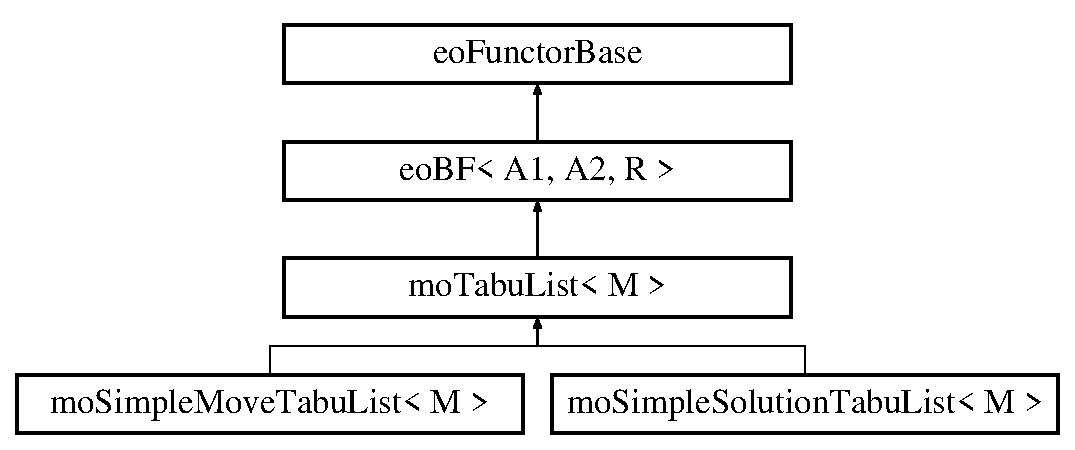
\includegraphics[height=3.88889cm]{classmo_tabu_list}
\end{center}
\end{figure}
\subsection*{Public Types}
\begin{CompactItemize}
\item 
typedef M::EOType {\bf EOT}\label{classmo_tabu_list_w0}

\begin{CompactList}\small\item\em Alias for the type. \item\end{CompactList}\end{CompactItemize}
\subsection*{Public Member Functions}
\begin{CompactItemize}
\item 
virtual void {\bf add} (const M \&\_\-move, const {\bf EOT} \&\_\-solution)=0
\begin{CompactList}\small\item\em Procedure to add a move in the tabu list. \item\end{CompactList}\item 
virtual void {\bf update} ()=0
\begin{CompactList}\small\item\em Procedure that updates the tabu list content. \item\end{CompactList}\item 
virtual void {\bf init} ()=0
\begin{CompactList}\small\item\em Procedure which initialises the tabu list. \item\end{CompactList}\end{CompactItemize}


\subsection{Detailed Description}
\subsubsection*{template$<$class M$>$ class mo\-Tabu\-List$<$ M $>$}

Class describing a tabu list that a {\bf mo\-TS}{\rm (p.\,\pageref{classmo_t_s})} uses. 

It is only a description, does nothing... A new object that herits from this class has to be defined in order to be used in a {\bf mo\-TS}{\rm (p.\,\pageref{classmo_t_s})}. 



Definition at line 46 of file mo\-Tabu\-List.h.

\subsection{Member Function Documentation}
\index{moTabuList@{mo\-Tabu\-List}!add@{add}}
\index{add@{add}!moTabuList@{mo\-Tabu\-List}}
\subsubsection{\setlength{\rightskip}{0pt plus 5cm}template$<$class M$>$ virtual void {\bf mo\-Tabu\-List}$<$ M $>$::add (const M \& {\em \_\-move}, const {\bf EOT} \& {\em \_\-solution})\hspace{0.3cm}{\tt  [pure virtual]}}\label{classmo_tabu_list_a0}


Procedure to add a move in the tabu list. 

The two parameters have not to be modified so they are constant parameters.

\begin{Desc}
\item[Parameters:]
\begin{description}
\item[{\em \_\-move}]a new tabu move. \item[{\em \_\-solution}]the origianl solution associated to this move. \end{description}
\end{Desc}


Implemented in {\bf mo\-Simple\-Move\-Tabu\-List$<$ M $>$} {\rm (p.\,\pageref{classmo_simple_move_tabu_list_a2})}, and {\bf mo\-Simple\-Solution\-Tabu\-List$<$ M $>$} {\rm (p.\,\pageref{classmo_simple_solution_tabu_list_a2})}.\index{moTabuList@{mo\-Tabu\-List}!update@{update}}
\index{update@{update}!moTabuList@{mo\-Tabu\-List}}
\subsubsection{\setlength{\rightskip}{0pt plus 5cm}template$<$class M$>$ virtual void {\bf mo\-Tabu\-List}$<$ M $>$::update ()\hspace{0.3cm}{\tt  [pure virtual]}}\label{classmo_tabu_list_a1}


Procedure that updates the tabu list content. 

Generally, a counter associated to each saved move is decreased by one. 

Implemented in {\bf mo\-Simple\-Move\-Tabu\-List$<$ M $>$} {\rm (p.\,\pageref{classmo_simple_move_tabu_list_a3})}, and {\bf mo\-Simple\-Solution\-Tabu\-List$<$ M $>$} {\rm (p.\,\pageref{classmo_simple_solution_tabu_list_a3})}.\index{moTabuList@{mo\-Tabu\-List}!init@{init}}
\index{init@{init}!moTabuList@{mo\-Tabu\-List}}
\subsubsection{\setlength{\rightskip}{0pt plus 5cm}template$<$class M$>$ virtual void {\bf mo\-Tabu\-List}$<$ M $>$::init ()\hspace{0.3cm}{\tt  [pure virtual]}}\label{classmo_tabu_list_a2}


Procedure which initialises the tabu list. 

Can be useful if the data structure needs to be allocated before being used. 

Implemented in {\bf mo\-Simple\-Move\-Tabu\-List$<$ M $>$} {\rm (p.\,\pageref{classmo_simple_move_tabu_list_a4})}, and {\bf mo\-Simple\-Solution\-Tabu\-List$<$ M $>$} {\rm (p.\,\pageref{classmo_simple_solution_tabu_list_a4})}.

The documentation for this class was generated from the following file:\begin{CompactItemize}
\item 
mo\-Tabu\-List.h\end{CompactItemize}

\section{moTS$<$ M $>$ Class Template Reference}
\label{classmo_t_s}\index{moTS@{moTS}}
Tabu Search (TS).  


{\tt \#include $<$moTS.h$>$}

Inherits {\bf moAlgo$<$ M::EOType $>$}.

\subsection*{Public Member Functions}
\begin{CompactItemize}
\item 
{\bf moTS} ({\bf moMoveInit}$<$ M $>$ \&\_\-move\_\-initializer, {\bf moNextMove}$<$ M $>$ \&\_\-next\_\-move\_\-generator, {\bf moMoveIncrEval}$<$ M $>$ \&\_\-incremental\_\-evaluation, {\bf moTabuList}$<$ M $>$ \&\_\-tabu\_\-list, {\bf moAspirCrit}$<$ M $>$ \&\_\-aspiration\_\-criterion, {\bf moSolContinue}$<$ {\bf EOT} $>$ \&\_\-continue, {\bf eoEvalFunc}$<$ {\bf EOT} $>$ \&\_\-full\_\-evaluation)
\begin{CompactList}\small\item\em Constructor of a \doxyref{moTS}{p.}{classmo_t_s} specifying all the boxes. \item\end{CompactList}\item 
{\bf moTS} ({\bf moMoveExpl}$<$ M $>$ \&\_\-move\_\-explorer, {\bf moSolContinue}$<$ {\bf EOT} $>$ \&\_\-continue, {\bf eoEvalFunc}$<$ {\bf EOT} $>$ \&\_\-full\_\-evaluation)
\begin{CompactList}\small\item\em Constructor with less parameters. \item\end{CompactList}\item 
bool {\bf operator()} ({\bf EOT} \&\_\-solution)
\begin{CompactList}\small\item\em {\bf Function} which launchs the Tabu Search. \item\end{CompactList}\end{CompactItemize}
\subsection*{Private Types}
\begin{CompactItemize}
\item 
typedef M::EOType {\bf EOT}\label{classmo_t_s_90d19d468c12ab5bd796948ce1ce79b1}

\begin{CompactList}\small\item\em Alias for the type. \item\end{CompactList}\item 
typedef EOT::Fitness {\bf Fitness}\label{classmo_t_s_aa0eefbb17111422e495d1255f876fca}

\begin{CompactList}\small\item\em Alias for the fitness. \item\end{CompactList}\end{CompactItemize}
\subsection*{Private Attributes}
\begin{CompactItemize}
\item 
{\bf moMoveExpl}$<$ M $>$ \& {\bf move\_\-explorer}\label{classmo_t_s_9fd948a2c586f1991f5a1eee927af8a6}

\begin{CompactList}\small\item\em Neighborhood explorer. \item\end{CompactList}\item 
{\bf moSolContinue}$<$ {\bf EOT} $>$ \& {\bf continu}\label{classmo_t_s_962a37393faf5239e657388d375cd9b3}

\begin{CompactList}\small\item\em Stop criterion. \item\end{CompactList}\item 
{\bf eoEvalFunc}$<$ {\bf EOT} $>$ \& {\bf full\_\-evaluation}\label{classmo_t_s_f44bb408007e2bff99f7a201842e8e48}

\begin{CompactList}\small\item\em Full evaluation function. \item\end{CompactList}\end{CompactItemize}


\subsection{Detailed Description}
\subsubsection*{template$<$class M$>$ class moTS$<$ M $>$}

Tabu Search (TS). 

Generic algorithm that describes a tabu search. 

Definition at line 50 of file moTS.h.

\subsection{Constructor \& Destructor Documentation}
\index{moTS@{moTS}!moTS@{moTS}}
\index{moTS@{moTS}!moTS@{moTS}}
\subsubsection{\setlength{\rightskip}{0pt plus 5cm}template$<$class M$>$ {\bf moTS}$<$ M $>$::{\bf moTS} ({\bf moMoveInit}$<$ M $>$ \& {\em \_\-move\_\-initializer}, {\bf moNextMove}$<$ M $>$ \& {\em \_\-next\_\-move\_\-generator}, {\bf moMoveIncrEval}$<$ M $>$ \& {\em \_\-incremental\_\-evaluation}, {\bf moTabuList}$<$ M $>$ \& {\em \_\-tabu\_\-list}, {\bf moAspirCrit}$<$ M $>$ \& {\em \_\-aspiration\_\-criterion}, {\bf moSolContinue}$<$ {\bf EOT} $>$ \& {\em \_\-continue}, {\bf eoEvalFunc}$<$ {\bf EOT} $>$ \& {\em \_\-full\_\-evaluation})\hspace{0.3cm}{\tt  [inline]}}\label{classmo_t_s_336408ddf8b7a29ffa8e01e9c18d8e10}


Constructor of a \doxyref{moTS}{p.}{classmo_t_s} specifying all the boxes. 

In this constructor, a \doxyref{moTSMoveLoopExpl}{p.}{classmo_t_s_move_loop_expl} is instanciated.

\begin{Desc}
\item[Parameters:]
\begin{description}
\item[{\em \_\-move\_\-initializer}]The move initializer. \item[{\em \_\-next\_\-move\_\-generator}]The neighbourhood explorer. \item[{\em \_\-incremental\_\-evaluation}]The (generally) efficient evaluation. \item[{\em \_\-tabu\_\-list}]The tabu list. \item[{\em \_\-aspiration\_\-criterion}]An aspiration criterion. \item[{\em \_\-continue}]The stopping criterion. \item[{\em \_\-full\_\-evaluation}]A full evaluation function. \end{description}
\end{Desc}


Definition at line 72 of file moTS.h.\index{moTS@{moTS}!moTS@{moTS}}
\index{moTS@{moTS}!moTS@{moTS}}
\subsubsection{\setlength{\rightskip}{0pt plus 5cm}template$<$class M$>$ {\bf moTS}$<$ M $>$::{\bf moTS} ({\bf moMoveExpl}$<$ M $>$ \& {\em \_\-move\_\-explorer}, {\bf moSolContinue}$<$ {\bf EOT} $>$ \& {\em \_\-continue}, {\bf eoEvalFunc}$<$ {\bf EOT} $>$ \& {\em \_\-full\_\-evaluation})\hspace{0.3cm}{\tt  [inline]}}\label{classmo_t_s_7e435fac1b8d5a410b7374d114e005e2}


Constructor with less parameters. 

The explorer is given in the parameters.

\begin{Desc}
\item[Parameters:]
\begin{description}
\item[{\em \_\-move\_\-explorer}]The explorer (generally different that a \doxyref{moTSMoveLoopExpl}{p.}{classmo_t_s_move_loop_expl}). \item[{\em \_\-continue}]The stopping criterion. \item[{\em \_\-full\_\-evaluation}]A full evaluation function. \end{description}
\end{Desc}


Definition at line 89 of file moTS.h.

\subsection{Member Function Documentation}
\index{moTS@{moTS}!operator()@{operator()}}
\index{operator()@{operator()}!moTS@{moTS}}
\subsubsection{\setlength{\rightskip}{0pt plus 5cm}template$<$class M$>$ bool {\bf moTS}$<$ M $>$::operator() ({\bf EOT} \& {\em \_\-solution})\hspace{0.3cm}{\tt  [inline, virtual]}}\label{classmo_t_s_2a011779723e24a5132a37593775bf56}


{\bf Function} which launchs the Tabu Search. 

Algorithm of the tabu search. As a \doxyref{moSA}{p.}{classmo_s_a} or a \doxyref{moHC}{p.}{classmo_h_c}, it can be used for HYBRIDATION in an evolutionary algorithm. For security a lock (pthread\_\-mutex\_\-t) is closed during the algorithm.

\begin{Desc}
\item[Parameters:]
\begin{description}
\item[{\em \_\-solution}]a solution to improve. \end{description}
\end{Desc}
\begin{Desc}
\item[Returns:]TRUE. \end{Desc}


Implements {\bf eoUF$<$ M::EOType \&, bool $>$}.

Definition at line 102 of file moTS.h.

References moTS$<$ M $>$::continu, moTS$<$ M $>$::full\_\-evaluation, and moTS$<$ M $>$::move\_\-explorer.

The documentation for this class was generated from the following file:\begin{CompactItemize}
\item 
moTS.h\end{CompactItemize}

\section{mo\-TSMove\-Loop\-Expl$<$ M $>$ Class Template Reference}
\label{classmo_t_s_move_loop_expl}\index{moTSMoveLoopExpl@{moTSMoveLoopExpl}}
Explorer for a Tabu Search algorithm.  


{\tt \#include $<$mo\-TSMove\-Loop\-Expl.h$>$}

Inheritance diagram for mo\-TSMove\-Loop\-Expl$<$ M $>$::\begin{figure}[H]
\begin{center}
\leavevmode
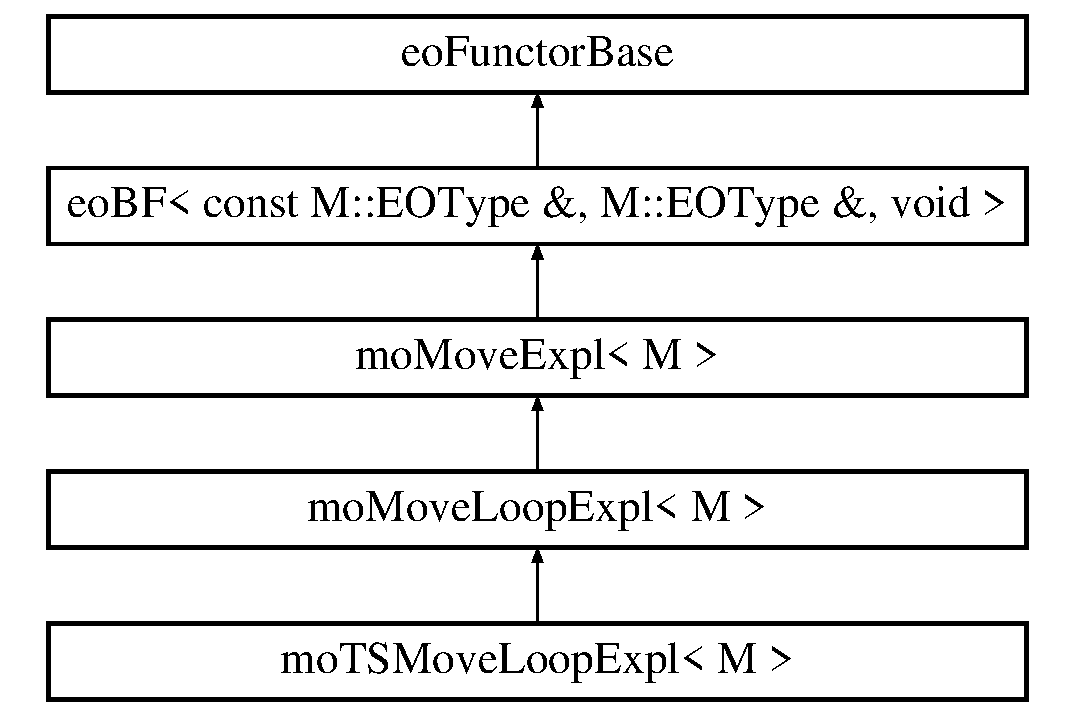
\includegraphics[height=5cm]{classmo_t_s_move_loop_expl}
\end{center}
\end{figure}
\subsection*{Public Member Functions}
\begin{CompactItemize}
\item 
\bf{mo\-TSMove\-Loop\-Expl} (\bf{mo\-Move\-Init}$<$ M $>$ \&\_\-move\_\-initializer, \bf{mo\-Next\-Move}$<$ M $>$ \&\_\-next\_\-move\_\-generator, \bf{mo\-Move\-Incr\-Eval}$<$ M $>$ \&\_\-incremental\_\-evaluation, \bf{mo\-Tabu\-List}$<$ M $>$ \&\_\-tabu\_\-list, \bf{mo\-Aspir\-Crit}$<$ M $>$ \&\_\-aspiration\_\-criterion)
\begin{CompactList}\small\item\em Constructor. \item\end{CompactList}\item 
void \bf{operator()} (const \bf{EOT} \&\_\-old\_\-solution, \bf{EOT} \&\_\-new\_\-solution)
\begin{CompactList}\small\item\em Procedure which lauches the exploration. \item\end{CompactList}\end{CompactItemize}
\subsection*{Private Types}
\begin{CompactItemize}
\item 
typedef M::EOType \bf{EOT}\label{classmo_t_s_move_loop_expl_47f42225e2ed096374b818bdb848a527}

\begin{CompactList}\small\item\em Alias for the type. \item\end{CompactList}\item 
typedef M::EOType::Fitness \bf{Fitness}\label{classmo_t_s_move_loop_expl_a1ba36c937b195ca2f7d1a24adaa7018}

\begin{CompactList}\small\item\em Alias for the fitness. \item\end{CompactList}\end{CompactItemize}
\subsection*{Private Attributes}
\begin{CompactItemize}
\item 
\bf{mo\-Move\-Init}$<$ M $>$ \& \bf{move\_\-initializer}\label{classmo_t_s_move_loop_expl_cd680d22382b9941d2c34133a641d443}

\begin{CompactList}\small\item\em Move initialisation. \item\end{CompactList}\item 
\bf{mo\-Next\-Move}$<$ M $>$ \& \bf{next\_\-move\_\-generator}\label{classmo_t_s_move_loop_expl_a2bbb593af2beefb05a307277c22b3d5}

\begin{CompactList}\small\item\em Neighborhood explorer. \item\end{CompactList}\item 
\bf{mo\-Move\-Incr\-Eval}$<$ M $>$ \& \bf{incremental\_\-evaluation}\label{classmo_t_s_move_loop_expl_491fa46e1cb7935cb515b27b85bf8765}

\begin{CompactList}\small\item\em Efficient evaluation. \item\end{CompactList}\item 
\bf{mo\-Best\-Impr\-Select}$<$ M $>$ \bf{move\_\-selection}\label{classmo_t_s_move_loop_expl_1caa6939fbe65ec4255e9e6dc3ce333b}

\begin{CompactList}\small\item\em Move selector. \item\end{CompactList}\item 
\bf{mo\-Tabu\-List}$<$ M $>$ \& \bf{tabu\_\-list}\label{classmo_t_s_move_loop_expl_0e5988a940ba218e87c53b7e56d79790}

\begin{CompactList}\small\item\em Tabu list. \item\end{CompactList}\item 
\bf{mo\-Aspir\-Crit}$<$ M $>$ \& \bf{aspiration\_\-criterion}\label{classmo_t_s_move_loop_expl_bdfc8efb22599c150b3c3d44cd416b09}

\begin{CompactList}\small\item\em Aspiration criterion. \item\end{CompactList}\end{CompactItemize}


\subsection{Detailed Description}
\subsubsection*{template$<$class M$>$ class mo\-TSMove\-Loop\-Expl$<$ M $>$}

Explorer for a Tabu Search algorithm. 

It is used by a \doxyref{mo\-TS}{p.}{classmo_t_s}. 



Definition at line 53 of file mo\-TSMove\-Loop\-Expl.h.

\subsection{Constructor \& Destructor Documentation}
\index{moTSMoveLoopExpl@{mo\-TSMove\-Loop\-Expl}!moTSMoveLoopExpl@{moTSMoveLoopExpl}}
\index{moTSMoveLoopExpl@{moTSMoveLoopExpl}!moTSMoveLoopExpl@{mo\-TSMove\-Loop\-Expl}}
\subsubsection{\setlength{\rightskip}{0pt plus 5cm}template$<$class M$>$ \bf{mo\-TSMove\-Loop\-Expl}$<$ M $>$::\bf{mo\-TSMove\-Loop\-Expl} (\bf{mo\-Move\-Init}$<$ M $>$ \& {\em \_\-move\_\-initializer}, \bf{mo\-Next\-Move}$<$ M $>$ \& {\em \_\-next\_\-move\_\-generator}, \bf{mo\-Move\-Incr\-Eval}$<$ M $>$ \& {\em \_\-incremental\_\-evaluation}, \bf{mo\-Tabu\-List}$<$ M $>$ \& {\em \_\-tabu\_\-list}, \bf{mo\-Aspir\-Crit}$<$ M $>$ \& {\em \_\-aspiration\_\-criterion})\hspace{0.3cm}{\tt  [inline]}}\label{classmo_t_s_move_loop_expl_be5cf0853777718c3bbcbef456b50bc7}


Constructor. 

\begin{Desc}
\item[Parameters:]
\begin{description}
\item[{\em \_\-move\_\-initializer}]The move initializer. \item[{\em \_\-next\_\-move\_\-generator}]The neighbourhood explorer. \item[{\em \_\-incremental\_\-evaluation}]A (generally) efficient evaluation. \item[{\em \_\-tabu\_\-list}]The tabu list. \item[{\em \_\-aspiration\_\-criterion}]An aspiration criterion. \end{description}
\end{Desc}


Definition at line 71 of file mo\-TSMove\-Loop\-Expl.h.

References mo\-TSMove\-Loop\-Expl$<$ M $>$::aspiration\_\-criterion, and mo\-TSMove\-Loop\-Expl$<$ M $>$::tabu\_\-list.

\subsection{Member Function Documentation}
\index{moTSMoveLoopExpl@{mo\-TSMove\-Loop\-Expl}!operator()@{operator()}}
\index{operator()@{operator()}!moTSMoveLoopExpl@{mo\-TSMove\-Loop\-Expl}}
\subsubsection{\setlength{\rightskip}{0pt plus 5cm}template$<$class M$>$ void \bf{mo\-TSMove\-Loop\-Expl}$<$ M $>$::operator() (const \bf{EOT} \& {\em \_\-old\_\-solution}, \bf{EOT} \& {\em \_\-new\_\-solution})\hspace{0.3cm}{\tt  [inline, virtual]}}\label{classmo_t_s_move_loop_expl_853743f2e21def3ea129556f47fafa55}


Procedure which lauches the exploration. 

The exploration continues while the chosen move is not in the tabu list or the aspiration criterion is true. If these 2 conditions are not true, the exploration stops if the move selector update function returns false.

\begin{Desc}
\item[Parameters:]
\begin{description}
\item[{\em \_\-old\_\-solution}]the initial solution \item[{\em \_\-new\_\-solution}]the new solution \end{description}
\end{Desc}


Implements \bf{eo\-BF$<$ const M::EOType \&, M::EOType \&, void $>$}.

Definition at line 90 of file mo\-TSMove\-Loop\-Expl.h.

References mo\-TSMove\-Loop\-Expl$<$ M $>$::aspiration\_\-criterion, mo\-TSMove\-Loop\-Expl$<$ M $>$::incremental\_\-evaluation, mo\-TSMove\-Loop\-Expl$<$ M $>$::move\_\-initializer, mo\-TSMove\-Loop\-Expl$<$ M $>$::move\_\-selection, mo\-TSMove\-Loop\-Expl$<$ M $>$::next\_\-move\_\-generator, and mo\-TSMove\-Loop\-Expl$<$ M $>$::tabu\_\-list.

The documentation for this class was generated from the following file:\begin{CompactItemize}
\item 
mo\-TSMove\-Loop\-Expl.h\end{CompactItemize}

\printindex
\end{document}
